\documentclass[12pt]{article}
\usepackage[utf8]{inputenc}
\usepackage{amsmath}
\usepackage{amsfonts}
\usepackage{amssymb}
\usepackage{graphicx}
\graphicspath{ {./img/} }
\usepackage{hyperref}
\usepackage{array}
\usepackage[table]{xcolor}
\usepackage{xcolor,colortbl}
\usepackage{multirow}
\usepackage{longtable}
\usepackage{enumitem}
\usepackage{fancyvrb}
\usepackage[a4paper, total={6in, 8in}]{geometry}

\usepackage{titlesec}

\setcounter{secnumdepth}{4}

\newcounter{mycounter} 
\newcommand\showmycounter{\stepcounter{mycounter}\themycounter}

\titleformat{\paragraph}
{\normalfont\normalsize\bfseries}{\theparagraph}{1em}{}
\titlespacing*{\paragraph}
{0pt}{3.25ex plus 1ex minus .2ex}{1.5ex plus .2ex}

\author{Natale Guadagno, Paolo Patrone}
\title{Requisites Analysis Document - TecStore}
\renewcommand{\contentsname}{Contenuti}

\usepackage{hyperref}
\hypersetup{
    colorlinks,
        citecolor=blue,
    filecolor=blue,
    linkcolor=blue,
    urlcolor=blue,
    linktocpage
}

\begin{document}

\maketitle
\newpage
\tableofcontents
\newpage
\newgeometry{a4paper,textwidth=345pt,textheight=598pt}
\section*{Partecipanti}
\begin{center}
\begin{tabular} {|c|c|}
\hline
\textbf{Nome} & \textbf{Matricola} \\
\hline
Guadagno Natale & 0512106546 \\
Patrone Paolo & 0512106153 \\
\hline
\end{tabular}
\end{center}


\section*{Revision History}
\begin{center}
\begin{tabular} {|c|c|c|}
\hline
\textbf{Data} & \textbf{Versione} & \textbf{Descrizione} \\
01/12/2021 & 0.1 & Prima stesura \\
02/12/2021 & 0.2 & Requisiti funzionali \\
\hline

\hline
\end{tabular}
\end{center}

\newpage

\section{Introduzione}

\subsection{Scopo del sistema}
Il sistema si pone l'obiettivo di facilitare le operazioni di gestione e controllo di operazioni di compravendita e di operazioni gestionali che non sono a carico dell'utenza, come la gestione del personale e dell'inventario. Sono previste viste e interfacce distinte per le varie operazioni per semplificare l'utilizzo ed evitare confusione.

\subsection{Ambito del sistema}
TecStore è una piattaforma web che permette ad utenti di comprare e vendere materiale tecnologico, che può essere messo in vendita da altri utenti o dalla piattaforma stessa. Trattandosi di un negozio piccolo, il catalogo è relativamente limitato, ma si punta a creare utenza attraverso prezzi vantaggiosi e un servizio clienti di qualità.
L'utenza della piattaforma si divide in:
\begin{itemize}
\item Clienti, che, una volta registrati ed autenticati, possono acquistare e vendere articoli
\item Centralinisti, che gestiscono i \emph{ticket} e autorizzano le vendite
\item Magazzinieri, che gestiscono le spedizioni degli articoli
\item Amministratori catalogo, che gestiscono gli articoli messi in vendita dalla piattaforma
\item Amministratori personale, che gestiscono la presenza nel sistema dei dipendenti
\end{itemize}

\subsection{Obiettivi del progetto}

\subsection{Definizioni, acronimi ed abbreviazioni}

\begin{itemize}
\item TecStore: nome della piattaforma 
\item Cliente: utente che può acquistare, vendere, richiedere assistenza
\item Centralinista: utente che controlla le vendite e fornisce assistenza ai clienti
\item Magazziniere: utente che controlla la spedizione degli ordini
\item Amministratore catalogo: utente che gestisce le vendite da parte della piattaforma
\item Amministratore personale: utente che gestisce gli account degli altri utenti, fatta eccezione per i clienti
\item DBMS: Database Management System, sistema di gestione di una base di dati
\item Ticket: strumento utilizzabile dai clienti per comunicare con il servizio clienti. È una comunicazione asincrona.
\end{itemize}

\section{Sistema proposto}
 
\subsection{Identificazione attori}
\begin{center}
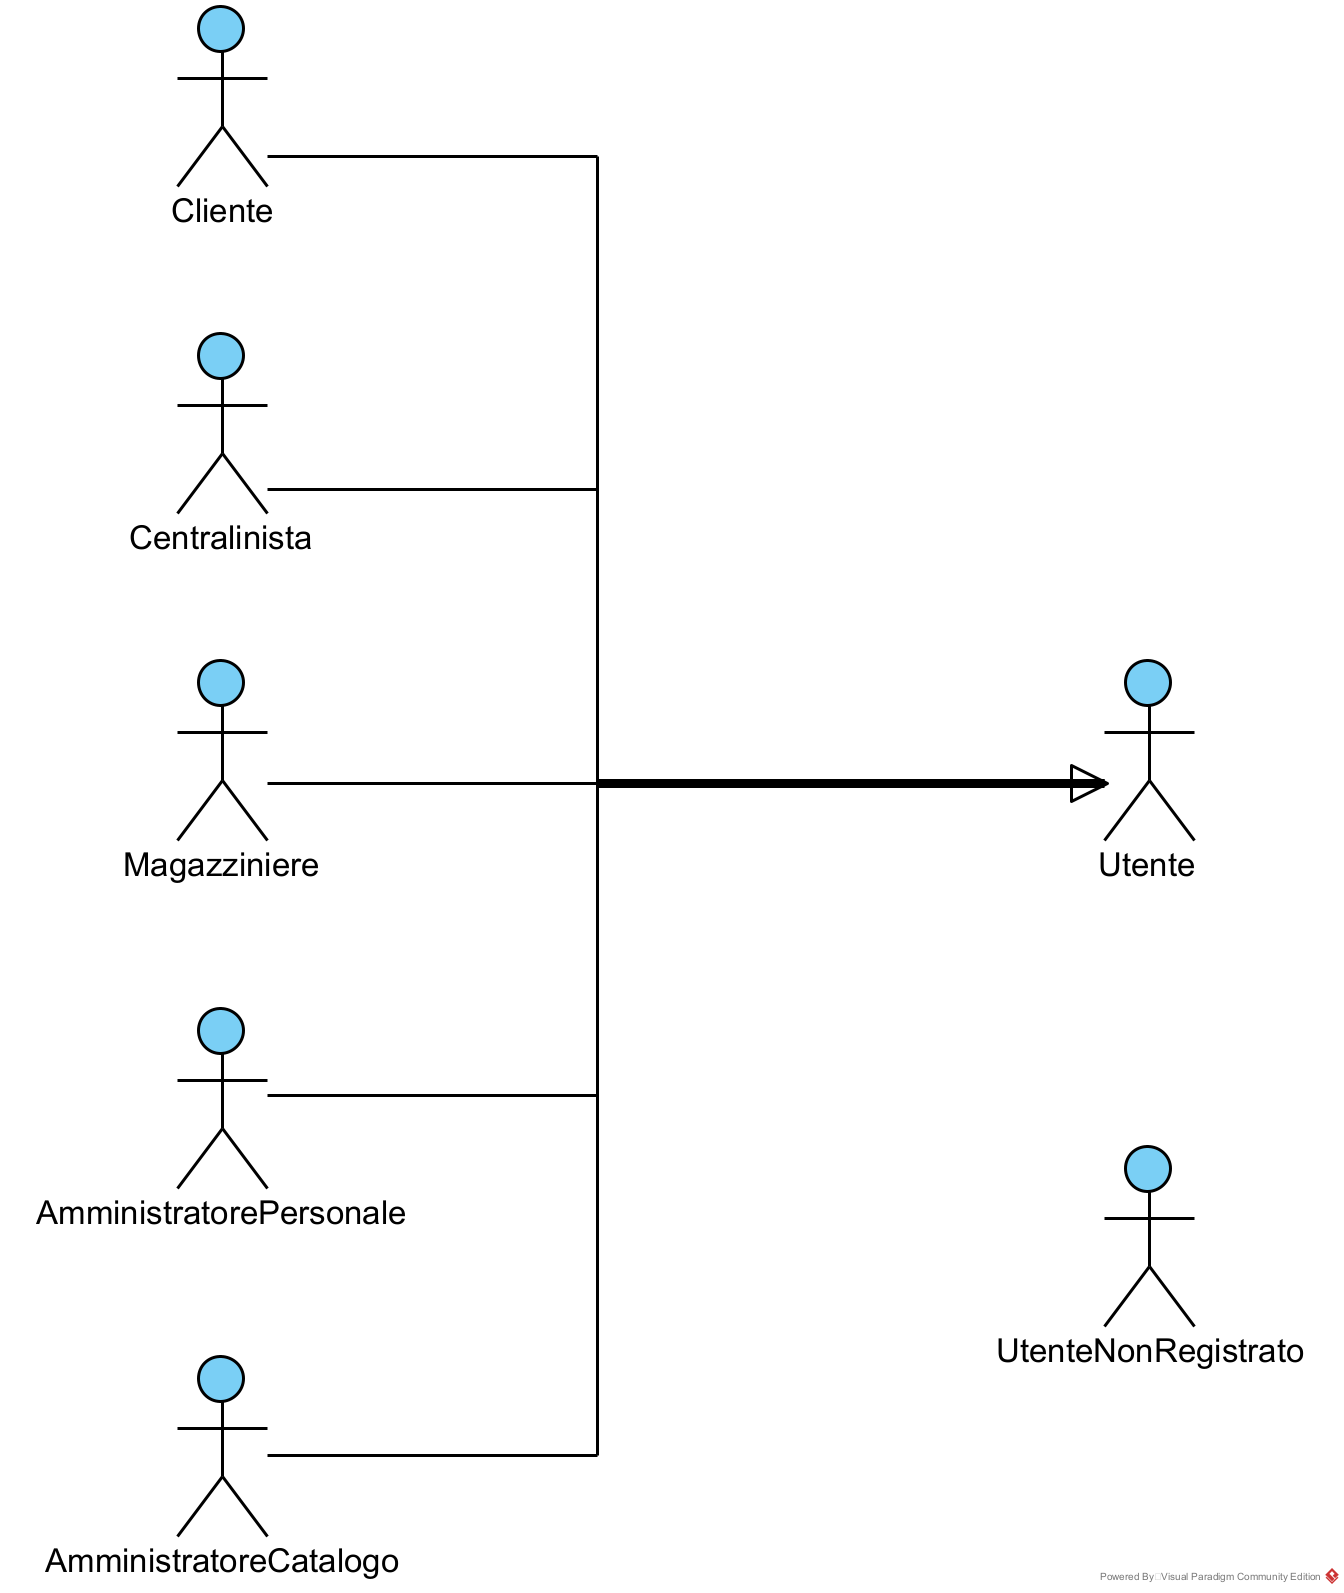
\includegraphics[width=\textwidth]{IdentificazioneAttori}
\end{center}
 
\newgeometry{top=0.5in,bottom=0.5in,right=0.5in,left=0.5in}
\subsection{Requisiti funzionali}
\begin{center}
\begin{tabular}{|c|l|c|}
\hline
\rowcolor[gray]{0.8}
\textbf{Funzionalità} & \textbf{Requisito} & \textbf{Priorità} \\
\hline
\multirow{8}{*}{Clienti} & 3.1.1 Registrazione & Alta \\
& 3.1.2 Autenticazione & Alta \\
& 3.1.3 Acquisto & Alta \\
& 3.1.4 Annullamento & Media \\
& 3.1.5 Vendita & Media \\
& 3.1.6 Assistenza & Alta \\
& 3.1.7 ModificaProfilo & Bassa \\
& 3.1.8 RecuperoPassword & Media \\
\hline
\multirow{5}{*}{Gestione} & 3.2.1 GestioneOrdini & Alta \\
& 3.2.2 GestioneTicket & Alta \\
& 3.2.3 ControlloArticoli & Alta \\
& 3.2.4 GestionePersonale & Alta \\
& 3.2.5 GestioneCatalogo & Alta \\

\hline
\end{tabular}
\end{center}

\subsubsection{Clienti}
Questa funzionalità racchiude tutte le operazioni fornite agli utenti.

\paragraph*{Registrazione}
\begin{center}
\begin{tabular}{|c|c|}
\rowcolor[gray]{0.8}
\hline
\textbf{Attore} & \textbf{Funzionalità} \\
Cliente non registrato & Permette di registrarsi. \\
\hline
\end{tabular}
\end{center}

\paragraph*{Autenticazione}
\begin{center}
\begin{tabular}{|c|c|}
\rowcolor[gray]{0.8}
\hline
\textbf{Attore} & \textbf{Funzionalità} \\
Cliente registrato & Permette di autenticarsi. \\
\hline
\end{tabular}
\end{center}

\paragraph*{Acquisto}
\begin{center}
\begin{tabular}{|c|c|}
\rowcolor[gray]{0.8}
\hline
\textbf{Attore} & \textbf{Funzionalità} \\
Cliente registrato & Permette di acquistare un articolo. \\
\hline
\end{tabular}
\end{center}

\paragraph*{Annullamento}
\begin{center}
\begin{tabular}{|c|c|}
\rowcolor[gray]{0.8}
\hline
\textbf{Attore} & \textbf{Funzionalità} \\
Cliente registrato & Permette di annullare un ordine. \\
\hline
\end{tabular}
\end{center}

\paragraph*{Vendita}
\begin{center}
\begin{tabular}{|c|c|}
\rowcolor[gray]{0.8}
\hline
\textbf{Attore} & \textbf{Funzionalità} \\
Cliente registrato & Permette di vendere un articolo. \\
\hline
\end{tabular}
\end{center}

\paragraph*{Assistenza}
\begin{center}
\begin{tabular}{|c|c|}
\rowcolor[gray]{0.8}
\hline
\textbf{Attore} & \textbf{Funzionalità} \\
Cliente registrato & Permette di richiedere assistenza. \\
\hline
\end{tabular}
\end{center}

\paragraph*{ModificaProfilo}
\begin{center}
\begin{tabular}{|c|c|}
\rowcolor[gray]{0.8}
\hline

% TODO
\textbf{Attore} & \textbf{Funzionalità} \\
Cliente registrato & Permette di modificare informazioni del profilo come password, carta di credito e indirizzo. \\
\hline
\end{tabular}
\end{center}

\paragraph*{RecuperoPassword}
\begin{center}
\begin{tabular}{|c|c|}
\rowcolor[gray]{0.8}
\hline
\textbf{Attore} & \textbf{Funzionalità} \\
Cliente registrato & Permette di modificare la password se la si è dimenticata. \\
\hline
\end{tabular}
\end{center}

\subsubsection{Gestione}
Questa funzionalità racchiude tutte le operazioni fornite al personale per la gestione della piattaforma.

\paragraph*{GestioneOrdini}
\begin{center}
\begin{tabular}{|c|c|}
\rowcolor[gray]{0.8}
\hline
\textbf{Attore} & \textbf{Funzionalità} \\
Magazziniere & Permette di confermare la spedizione di un ordine o di annullarlo. \\
\hline
\end{tabular}
\end{center}

\paragraph*{GestioneTicket}
\begin{center}
\begin{tabular}{|c|c|}
\rowcolor[gray]{0.8}
\hline
\textbf{Attore} & \textbf{Funzionalità} \\
Centralinista & Permette di interagire con gli utenti per risolvere un problema. \\
\hline
\end{tabular}
\end{center}

\paragraph*{ControlloArticoli}
\begin{center}
\begin{tabular}{|c|c|}
\rowcolor[gray]{0.8}
\hline
\textbf{Attore} & \textbf{Funzionalità} \\
Centralinista & Permette di filtrare quali articoli messi in vendita vengono accettati. \\
\hline
\end{tabular}
\end{center}

\paragraph*{GestionePersonale}
\begin{center}
\begin{tabular}{|c|c|}
\rowcolor[gray]{0.8}
\hline
\textbf{Attore} & \textbf{Funzionalità} \\
Amministratore personale & Permette di aggiungere, rimuovere e modificare account per i dipendenti. \\
\hline
\end{tabular}
\end{center}

\paragraph*{GestioneCatalogo}
\begin{center}
\begin{tabular}{|c|c|}
\rowcolor[gray]{0.8}
\hline
\textbf{Attore} & \textbf{Funzionalità} \\
Amministratore catalogo & Permette di aggiungere, rimuovere e modificare articoli venduti da TecStore. \\
\hline
\end{tabular}
\end{center}

\newpage


\newgeometry{a4paper,textwidth=345pt,textheight=598pt}
\subsection{Requisiti non funzionali}
\subsubsection{Sicurezza e privacy}
Il sistema deve prevedere tutte le pratiche di sicurezza fondamentali, come l'utilizzo di SSL per la trasmissione dei dati, l'utilizzo di \textit{hashing} e \textit{salt} per le password memorizzate nel database, tutti i dati delle carte di credito e anagrafiche devono essere cifrati prima di essere inseriti nel database utilizzando una cifratura robusta con una chiave che non deve essere esposta pubblicamente per nessun motivo. \\
In caso di tentativo di accesso a schermate riservate da parte di un utente consumatore o viceversa, ovvero un utente del personale che cerca di accedere al catalogo, deve essere previsto un avviso e un \textit{redirect} ad una pagina correttamente accessibile da quel tipo di utente.

\subsubsection{Affidabilità}
Il sistema deve garantire un \emph{uptime} di almeno il 99.9\%, ovvero un \textit{downtime} annualizzato di meno di 9 ore. Ciò è cruciale per far sì che l'utenza non venga scoraggiata dall'utilizzo di TecStore come negozio primario, creando perdite potenziali molto alte. \footnote{https://www.the20.com/blog/the-cost-of-it-downtime/}

\subsubsection{Performance}
Il sistema deve prevedere la possibilità di utilizzo di sistemi di \textit{load balancing} per distribuire il carico di utenza in caso di picchi improvvisi tra più server, in modo da garantire l'uso della piattaforma al maggior numero di clienti possibile.

\subsubsection{Manutenibilità}
Il sistema sarà progettato secondo principi di sviluppo che ne garantiranno la semplicità di aggiornamento, ampliamento e modifica.
Sarà utilizzata un'architettura Three-Tier per separare la gestione dei dati, il programma server e l'interfaccia utente.

\subsection{Implementazione}
Sarà utilizzata la tecnologia JSP con servlet su server Tomcat per la presentazione delle pagine web all'utente , un database MariaDB per la memorizzazione dei dati e ogni utente utilizzerà un comune browser web per accedere al sistema.

\newpage
\subsection{Scenari}
\subsubsection{Cliente non registrato vuole acquistare un articolo}
Un nuovo cliente, Mario Rossi, apre il sito per la prima volta.
Inserisce nella barra di ricerca il nome dell'articolo a cui è interessato, ``Mouse".
Dall'elenco dei risultati, sceglie quello che più gli interessa e fa click su di esso.
Dalla pagina dei dettagli che viene caricata, convinto dalle specifiche del mouse, decide di acquistarlo e fa click su ``Aggiungi al carrello".
Dato che non è autenticato viene chiesto di autenticarsi o registrarsi per proseguire con l'operazione.
Decide di registrarsi, inserendo quindi email ``mariorossi@email.tld", password ``6GksD-3Sc", nome ``Mario", cognome ``Rossi", indirizzo ``Via Roma 1, Torino". Fa click su ``Conferma".
Viene quindi rimandato alla pagina del carrello con il nuovo articolo appena inserito e fa click su ``Acquista" per proseguire con l'acquisto.
Inserisce i dati della carta di credito, come numero  ``4485518752812161", scadenza "02/27", CVV ``458" e ``Italiana" come nazionalità e fa click su ``Conferma".
L'ordine viene quindi inserito nel sistema in attesa di spedizione da parte di un magazziniere.
Il giorno successivo Luigi Verdi, magazziniere, si connette al sistema, si autentica e dall'elenco degli ordini seleziona quello di Mario. Procura l'articolo dal magazzino, lo imballa, prenota il corriere per il ritiro, inserisce il codice del \emph{tracking} e conferma la spedizione dell'ordine.

\subsubsection{Cliente registrato vuole acquistare un articolo}
Un cliente già registrato, Mario Rossi apre il sito e inserisce nella barra di ricerca il nome dell'articolo a cui è interessato, ``Tastiera".
Dall'elenco dei risultati, sceglie quella che più gli interessa e fa click su di esso.
Dalla pagina dei dettagli che viene caricata, convinto dalle specifiche della tastiera, decide di acquistarla e fa click su ``Aggiungi al carrello".
Dato che non è autenticato viene chiesto di autenticarsi o registrarsi per proseguire con l'operazione.
Essendo già registrato, si autentica con email ``mariorossi@email.tld" e password ``6GksD-3Sc".
Viene quindi rimandato alla pagina del carrello con il nuovo articolo appena inserito e fa click su ``Acquista" per proseguire con l'acquisto.
Avendo già acquistato in precedenza, le informazioni della sua carta di credito sono già memorizzate nel sistema.
L'ordine viene quindi inserito nel sistema in attesa di spedizione da parte di un magazziniere.
Il giorno successivo Luigi Verdi, magazziniere, si connette al sistema, si autentica e dall'elenco degli ordini seleziona quello di Mario. Procura l'articolo dal magazzino, lo imballa, prenota il corriere per il ritiro, inserisce il codice del \emph{tracking} e conferma la spedizione dell'ordine.

\subsubsection{Cliente annulla ordine}
Un cliente già registrato, Mario Rossi apre il sito e inserisce nella barra di ricerca il nome dell'articolo a cui è interessato, ``Tastiera".
Dall'elenco dei risultati, sceglie quella che più gli interessa e fa click su di esso.
Dalla pagina dei dettagli che viene caricata, convinto dalle specifiche della tastiera, decide di acquistarla e fa click su ``Aggiungi al carrello".
Dato che non è autenticato viene chiesto di autenticarsi o registrarsi per proseguire con l'operazione.
Essendo già registrato, si autentica con email ``mariorossi@email.tld" e password ``6GksD-3Sc".
Avendo già acquistato in precedenza, le informazioni della sua carta di credito sono già memorizzate nel sistema.
L'ordine viene quindi inserito nel sistema in attesa di spedizione da parte di un magazziniere.
Pochi minuti dopo, cambia idea sull'acquisto effettuato e decide di annullare l'ordine.
Dalla pagina principale fa click su ``Storico ordini" e dall'elenco degli ordini fa click su ``Annulla" per la tastiera.
Dato che non è ancora stato spedita, l'ordine viene annullato.

\newpage

\subsubsection{Cliente modifica informazioni profilo}
Un cliente già registrato, Mario Rossi, si è appena trasferito. Per far sì che i nuovi ordini da lui effettuati vengano spediti alla sua nuova casa, decide di modificare le informazioni del suo profilo sulla piattaforma.
Essendo già registrato, si autentica con email ``mariorossi@email.tld" e password ``6GksD-3Sc".
Dalla pagina iniziale fa click su ``Modifica profilo".
Nel modulo che gli viene presentato inserisce il nuovo indirizzo e fa click su ``Conferma".

\subsubsection{Cliente modifica password}
Un cliente già registrato, Mario Rossi, decide di modificare la sua password. 
Si autentica con email ``mariorossi@email.tld" e password ``6GksD-3Sc".
Dalla pagina iniziale fa click su ``Modifica profilo" e su ``Modifica password".
Nel modulo che gli viene presentato inserisce la nuova password ``2eyccH4jj4a" e fa click su conferma.

\subsubsection{Cliente recupera password}
Un cliente già registrato, Mario Rossi, ha dimenticato la sua password.
Dal modulo per l'autenticazione fa click su ``Password dimenticata?" e inserisce il suo indirizzo email.
Usando il link che gli viene spedito, viene rimandato al modulo per la modifica della password. Inserisce quindi ``edNdnP48D7q" e fa click su ``Conferma".

\subsubsection{Cliente apre ticket}
Un cliente già registrato, Mario Rossi, non ha ricevuto il suo ordine dopo oltre due settimane di attesa. Decide quindi di comunicare con l'assistenza.
Entra sul sito, fa click su ``Autenticati" e inserisce i suoi dati, email ``mariorossi@email.tld" e password ``edNdnP48D7q" e fa click su ``Autenticati".
Fa quindi click su ``Servizio clienti" e su ``Nuovo ticket".
Sceglie come tipologia ``Ordine effettuato" e inserisce come messaggio ``Non ho ricevuto il mio ordine dopo oltre due settimane".
Qualche ora dopo Anna Bianchi, centralinista, si autentica e vede il ticket di Mario, lo apre e, dopo aver contattato il corriere per sollecitare la spedizione, cerca di rassicurare Mario, scrivendo ``Caro Signor Rossi, ho parlato personalmente con il corriere che mi ha assicurato che il pacco Le sarà recapitato entro le prossime 48 ore.".
Il giorno successivo Mario riceve l'articolo e chiude il ticket.

\subsubsection{Cliente vende un articolo}
Un cliente già registrato, Carlo Neri, vuole vendere degli articoli. Dopo essersi autenticato con le credenziali ``carloneri@email.tld" e ``cVqFD4cSjRX", fa click su ``Area venditori".
Da qui fa click su ``Nuova vendita" e inserisce nel modulo come nome ``Webcam 3.1 MP 1080p 30fps", ``5" come quantità disponibile e ``21.00" come prezzo, ``Webcam alta qualità universale USB, compatibile con tutti i computer e sistemi operativi" come descrizione e aggiunge alcune foto. Fa click su ``Conferma" e l'articolo viene inserito nel sistema in attesa di verifica da parte di un centralinista.
Qualche ora dopo Anna Bianchi, centralinista, si autentica e vede la richiesta di vendita creata da Carlo. Dopo aver letto con cura le informazioni e guardato le foto, decide di accettare la vendita. L'articolo diventa quindi visualizzabile da chiunque ricerchi ``Webcam" sul sito.

\subsubsection{Cliente modifica una vendita}
Un cliente già registrato, Carlo Neri, vuole modificare i dettagli di una vendita. Dopo essersi autenticato con le credenziali ``carloneri@email.tld" e ``cVqFD4cSjRX", fa click su ``Area venditori" e fa click su ``Modifica" per la vendita interessata, ``Webcam".
Nel modulo, cambia il nome da ``Webcam 3.1 MP 1080p 30fps" a ``Webcam 3.1 MP 1080p \textbf{60fps}". Fa click su ``Conferma".
La vendita torna in attesa di verifica da parte di un centralinista.
Qualche ora dopo Anna Bianchi, centralinista, si autentica e vede la richiesta di modifica creata da Carlo. Dopo aver letto con cura le informazioni, decide di accettare la vendita. L'articolo diventa quindi visualizzabile da chiunque ricerchi ``Webcam" sul sito.

\subsubsection{Cliente annulla una vendita}
Un cliente già registrato, Carlo Neri, vuole annullare una vendita. Dopo essersi autenticato con le credenziali ``carloneri@email.tld" e ``cVqFD4cSjRX", fa click su ``Area venditori" e fa click su ``Annulla" per la vendita interessata, ``Webcam".
Dato che la vendita non è ancora stata accettata, viene immediatamente cancellata dal sito.

\subsubsection{Amministratore personale aggiunge un dipendente}
L'amministratore personale Alfonso Autori deve creare un nuovo account per il nuovo dipendente Carlo Abbamonti.
Apre la pagina iniziale e fa click su ``Autenticati".
Inserisce l'email: "alfosoautori@email.tld", e la password: "BWuCega2LV".
Viene reindirizzato alla pagina principale per l'amministratore, clicca su "Aggiungi Nuovo Dipendente".
Nella pagina di "Modulo nuovo dipendente" inserisce i dati del nuovo dipendente,
Nome: ``Carlo" , Cognome: ``Abbamonti", 
Email: ``carloabbamonti@email.tld",
CodiceFiscale: ``BBMCRL82A10H703R"
Via: `` Libertà", Numero civico: ``1", Città: ``Salerno", Provincia: ``SA", CAP: ``84122"
Tipologia: ``Centralinista".
Fa clic sul tasto "Conferma" e gli appare la pagina di conferma contenente le informazioni di accesso per Carlo.

\subsubsection{Amministratore personale modifica dipendente}
L'amministratore personale Alfonso Autori deve modificare l'indirizzo del dipendente Carlo Abbamonti.
Apre la pagina iniziale e fa click su ``Autenticati".
Inserisce l'email: "alfosoautori@email.tld", e la password: "BWuCega2LV".
Viene reindirizzato alla pagina principale per l'amministratore, 
clicca sul campo di ricerca ed inserisce: ``Abbamonti".
Gli vengono caricati tutti i risultati inerenti alla ricerca e trova il dipendente interessato. Alfonso fa click sul suo nome e visualizza i dettagli.
Nella pagina dei dettagli clicca sulla voce ``Modifica Dipendente".
Nalla sezione "Indirizzo" seleziona la voce ``Numero civico" ed inserisce "4" e in ``Via" inserisce ``Fiume".
Fa click su ``Conferma" e gli viene mostrata la pagina di avvenuta modifica dei dati.

\subsubsection{Amministratore personale rimuove dipendente}
L'amministratore personale Alfonso Autori deve rimuovere l'account del dipendente Carlo Abbamonti.
Apre la pagina iniziale e fa click su ``Autenticati".
Inserisce l'email: "alfosoautori@email.tld", e la password: "BWuCega2LV".
Viene reindirizzato alla pagina principale per l'amministratore, 
clicca sul campo di ricerca ed inserisce: ``Abbamonti".
Gli vengono caricati tutti i risultati inerenti alla ricerca e trova il dipendente interessato. Alfonso fa click sul suo nome e visualizza i dettagli.
Fa quindi click sulla voce "Elimina Dipendente", e gli appare la pagina di conferma di operazione avvenuta.

\subsubsection{Amministratore catalogo inserisce nuovo articolo}
L'amministratore del catalogo Tommaso Foggia deve inserire un nuovo articolo al catalogo.
Tommaso, detto "Tommy", apre la pagina iniziale e fa click su ``Autenticati".
Inserisce l'email: "tommyfoggia@email.tld", e la password: "tTV9wAKhJB".
Viene reindirizzato alla pagina principale per l'amministratore.
Clicca su "Inserisci Nuovo Articolo" e nel modulo per l'inserimento inserisce del campi, Nome: ``Tappetino RGB, Zero Gravity", Descrizione: ``Tappetino ultra leggero RGB, 2W/h, presa USB",
Quantità: ``2", Prezzo ``30.00".
Fa click su ``Conferma" e gli viene mostrata una pagina con messaggio ``Inserimento avvenuto con successo".

\newpage

\subsubsection{Amministratore catalogo modifica articolo}
L'amministratore del catalogo Tommaso Foggia deve modificare un articolo dal catalogo.
Tommaso, detto "Tommy", apre la pagina iniziale e fa click su ``Autenticati".
Inserisce l'email: "tommyfoggia@email.tld", e la password: "tTV9wAKhJB".
Viene reindirizzato alla pagina principale per l'amministratore.
clicca sul campo di ricerca ed inserisce: "HP Pavillion".
Gli vengono caricati tutti i risultati inerenti alla ricerca effettuata.
L'amministratore seleziona l'articolo interessato ed apre i dettagli.
Nella pagina dei dettagli clicca sulla voce ``Modifica Articolo",
alla sezione ``Prezzo" seleziona ed inserisce ``799.00".
Fa click su ``Conferma" e gli viene mostrata una pagina con messaggio ``Modifica avvenuta con successo".

\subsubsection{Amministratore catalogo rimuove articolo}
L'amministratore del catalogo Tommaso Foggia deve rimuovere un articolo dal catalogo.
Tommaso, detto "Tommy", apre la pagina iniziale e fa click su ``Autenticati".
Inserisce l'email: "tommyfoggia@email.tld", e la password: "tTV9wAKhJB".
Viene reindirizzato alla pagina principale per l'amministratore.
clicca sul campo di ricerca ed inserisce: "HP Pavillion".
Gli vengono caricati tutti i risultati inerenti alla ricerca effettuata.
L'amministratore seleziona l'articolo interessato ed apre i dettagli.
Nella pagina dei dettagli clicca sulla voce "Elimina Articolo",
Fa click su ``Conferma" e gli viene mostrata una pagina con messaggio ``Rimozione avvenuta con successo".


\newpage

\newgeometry{top=0.5in,bottom=0.5in,right=0.5in,left=0.5in}
\section{Use case}
\subsection{Comuni}
\subsubsection{Autenticazione}
\label{UC:autenticazione}
\begin{tabular}{|>{\columncolor[gray]{0.8}}c|p{12cm}|}
\hline
\textbf{ID} &UC\showmycounter \bigskip\showmycounter \bigskip Autenticazione \\
\hline
\textbf{Descrizione} & Un utente si autentica. \\
\hline
\textbf{Partecipanti} & Utente \\
\hline
\textbf{Condizione d'ingresso} & Un utente già registrato (\ref{UC:registrazione}) si connette al sito e vuole autenticarsi. \\
\hline
\textbf{Flusso di eventi} &
\begin{minipage}{12cm}
\begin{tabular}{p{5.5cm} p{5.5cm}}
\textbf{Cliente} & \textbf{Sistema} \\
Si collega al sito e da una pagina qualsiasi fa click sul tasto ``Autenticati". & \\
	& Mostra all'utente un modulo per l'inserimento di email e password. \\
Inserisce i dati richiesti e fa click su ``Autenticati". & \\
	& Se le credenziali sono corrette, rimanda l'utente alla pagina opportuna.
\end{tabular}
\end{minipage} \\
\hline
\textbf{Condizione d'uscita} & L'utente risulta autenticato per quella sessione. \\
\hline
\end {tabular}
\\


\subsection{Clienti}
\subsubsection{Registrazione}
\label{UC:registrazione}
\begin{tabular}{|>{\columncolor[gray]{0.8}}c|p{12cm}|}
\hline
\textbf{ID} &UC\showmycounter \bigskip\showmycounter \bigskip Registrazione \\
\hline
\textbf{Descrizione} & Un nuovo cliente si registra. \\
\hline
\textbf{Partecipanti} & Cliente non registrato \\
\hline
\textbf{Condizione d'ingresso} & Un nuovo cliente visita il sito per la prima volta e vuole registrarsi. \\
\hline
\textbf{Flusso di eventi} &
\begin{minipage}{12cm}
\begin{tabular}{p{5.5cm} p{5.5cm}}
\textbf{Cliente non registrato} & \textbf{Sistema} \\
Si collega al sito e da una pagina fa click sul tasto ``Registrati" & \\
& Mostra al cliente il form per la registrazione in cui inserire tutti i dati personali, come nome, cognome, indirizzo, email e password. \\
Inserisce tutti i dati richiesti e fa click su "Registrati". & \\
& Invia al cliente una mail di conferma e visualizza al cliente un messaggio con l'esito della registrazione. \\
\end{tabular}
\end{minipage} \\

\hline
\textbf{Condizione d'uscita} & Le informazioni del cliente vengono memorizzate nel sistema. \\
\hline
\end {tabular}
\\


\subsubsection{Ricerca}
\label{UC:ricerca}
\begin{tabular}{|>{\columncolor[gray]{0.8}}c|p{12cm}|}
\hline
\textbf{ID} &UC\showmycounter \bigskip Ricerca \\
\hline
\textbf{Descrizione} & Un cliente ricerca una parola chiave. \\
\hline
\textbf{Partecipanti} & Cliente \\
\hline
\textbf{Condizione d'ingresso} & Un cliente vuole scoprire il prezzo di un articolo. \\
\hline
\textbf{Flusso di eventi} &
\begin{minipage}{12cm}
\begin{tabular}{p{5.5cm} p{5.5cm}}
\textbf{Cliente} & \textbf{Sistema} \\
Da una pagina qualsiasi, digita il nome dell'articolo desiderato nella barra di ricerca e preme sul tasto ``Cerca". \\
	& Mostra all'utente un elenco di risultati pertinenti alla parola cercata. \\
\end{tabular}
\end{minipage} \\
\hline
\textbf{Condizione d'uscita} & All'utente viene mostrato un elenco di articoli in base alla parola chiave utilizzata. \\
\hline
\end {tabular}
\\

\subsubsection{Selezione}
\label{UC:selezione}
\begin{tabular}{|>{\columncolor[gray]{0.8}}c|p{12cm}|}
\hline
\textbf{ID} &UC\showmycounter \bigskip Selezione \\
\hline
\textbf{Descrizione} & Un cliente seleziona un articolo per visualizzarne i dettagli.  \\
\hline
\textbf{Partecipanti} & Cliente \\
\hline
\textbf{Condizione d'ingresso} & Un cliente ha effettuato una ricerca (\ref{UC:ricerca}) e vuole più informazioni su uno dei risultati. \\
\hline
\textbf{Flusso di eventi} &
\begin{minipage}{12cm}
\begin{tabular}{p{5.5cm} p{5.5cm}}
\textbf{Cliente} & \textbf{Sistema} \\
Seleziona uno dei risultati. \\
	& Visualizza i dettagli dell'articolo. \\
\end{tabular}
\end{minipage} \\
\hline
\textbf{Condizione d'uscita} & All'utente vengono mostrati i dettagli dell'articolo selezionato. \\
\hline
\end {tabular}
\\

\subsubsection{Aggiunta al carrello}
\label{UC:carrelloadd}
\begin{tabular}{|>{\columncolor[gray]{0.8}}c|p{12cm}|}
\hline
\textbf{ID} &UC\showmycounter \bigskip AggiuntaAlCarrello \\
\hline
\textbf{Descrizione} & Un cliente aggiunge un articolo al carrello.  \\
\hline
\textbf{Partecipanti} & Cliente \\
\hline
\textbf{Condizione d'ingresso} & Un cliente autenticato (\ref{UC:autenticazione}) ha effettuato una ricerca (\ref{UC:ricerca}) ed ha selezionato un articolo (\ref{UC:selezione} ed è interessato ad acquistare. \\
\hline
\textbf{Flusso di eventi} &
\begin{minipage}{12cm}
\begin{tabular}{p{5.5cm} p{5.5cm}}
\textbf{Cliente} & \textbf{Sistema} \\
Fa click su ``Aggiungi al carrello". \\
	& Mostra all'utente il contenuto del carrello. \\
\end{tabular}
\end{minipage} \\
\hline
\textbf{Condizione d'uscita} & L'aggiunta al carrello viene memorizzata. \\
\hline
\end {tabular}
\\

\subsubsection{Acquisto}
\label{UC:carrellobuy}
\begin{tabular}{|>{\columncolor[gray]{0.8}}c|p{12cm}|}
\hline
\textbf{ID} &UC\showmycounter \bigskip Acquisto \\
\hline
\textbf{Descrizione} & Un cliente acquista gli articoli presenti nel suo carrello.  \\
\hline
\textbf{Partecipanti} & Cliente \\
\hline
\textbf{Condizione d'ingresso} & Un cliente autenticato (\ref{UC:autenticazione}) ha aggiunto un articolo al carrello (\ref{UC:carrelloadd}). Ora vuole procedere con l'acquisto. \\
\hline
\textbf{Flusso di eventi} &
\begin{minipage}{12cm}
\begin{tabular}{p{5.5cm} p{5.5cm}}
\textbf{Cliente} & \textbf{Sistema} \\
Da una pagina qualsiasi, fa click su ``Carrello".
	& Mostra all'utente il contenuto del carrello. \\
Fa click su ``Acquista". \\
	& Crea un ordine nel sistema con stato ``InAttesa".
\end{tabular}
\end{minipage} \\
\hline
\textbf{Condizione d'uscita} & L'ordine viene creato. \\
\hline
\end {tabular}
\\

\subsubsection{Rimozione dal carrello}
\label{UC:carrelloremove}
\begin{tabular}{|>{\columncolor[gray]{0.8}}c|p{12cm}|}
\hline
\textbf{ID} &UC\showmycounter \bigskip RimozioneDalCarrello \\
\hline
\textbf{Descrizione} & Un cliente rimuove uno degli articoli presenti nel suo carrello.  \\
\hline
\textbf{Partecipanti} & Cliente \\
\hline
\textbf{Condizione d'ingresso} & Un cliente autenticato (\ref{UC:autenticazione}) ha aggiunto un articolo al carrello (\ref{UC:carrelloadd}). Ora vuole rimuoverlo. \\
\hline
\textbf{Flusso di eventi} &
\begin{minipage}{12cm}
\begin{tabular}{p{5.5cm} p{5.5cm}}
\textbf{Cliente} & \textbf{Sistema} \\
Da una pagina qualsiasi, fa click su ``Carrello".
	& Mostra all'utente il contenuto del carrello. \\
Fa click su ``Rimuovi" per l'articolo interessato.
	& Mostra all'utente una pagina di conferma. \\
\end{tabular}
\end{minipage} \\
\hline
\textbf{Condizione d'uscita} & L'articolo viene rimosso dal carrello. \\
\hline
\end {tabular}
\\

\subsubsection{Storico ordini}
\label{UC:storicoordini}
\begin{tabular}{|>{\columncolor[gray]{0.8}}c|p{12cm}|}
\hline
\textbf{ID} &UC\showmycounter \bigskip StoricoOrdini \\
\hline
\textbf{Descrizione} & Un cliente visualizza lo storico degli ordini effettuati.  \\
\hline
\textbf{Partecipanti} & Cliente \\
\hline
\textbf{Condizione d'ingresso} & Un cliente autenticato (\ref{UC:autenticazione}) è nella pagina iniziale. \\
\hline
\textbf{Flusso di eventi} &
\begin{minipage}{12cm}
\begin{tabular}{p{5.5cm} p{5.5cm}}
\textbf{Cliente} & \textbf{Sistema} \\
Fa click su ``Storico ordini". \\
	& Mostra all'utente una barra di ricerca per gli ordini. \\
Inserisce la parola chiave interessata. \\
	& Mostra all'utente un elenco di ordini corrispondenti. \\
\end{tabular}
\end{minipage} \\
\hline
\textbf{Condizione d'uscita} & Il cliente visualizza l'elenco degli ordini. \\
\hline
\end {tabular}

\subsubsection{Dettagli ordine}
\label{UC:dettagliordine}
\begin{tabular}{|>{\columncolor[gray]{0.8}}c|p{12cm}|}
\hline
\textbf{ID} &UC\showmycounter \bigskip DettagliOrdine \\
\hline
\textbf{Descrizione} & Un cliente visualizza i dettagli di un ordine.  \\
\hline
\textbf{Partecipanti} & Cliente \\
\hline
\textbf{Condizione d'ingresso} & Un cliente autenticato (\ref{UC:autenticazione}) è nello storico degli ordini (\ref{UC:storicoordini}). \\
\hline
\textbf{Flusso di eventi} &
\begin{minipage}{12cm}
\begin{tabular}{p{5.5cm} p{5.5cm}}
\textbf{Cliente} & \textbf{Sistema} \\
Fa click su ``Dettagli" per l'articolo interessato. \\
	& Mostra all'utente i dettagli dell'ordine selezionato.
\end{tabular}
\end{minipage} \\
\hline
\textbf{Condizione d'uscita} & Il cliente visualizza i dettagli dell'ordine selezionato. \\
\hline
\end {tabular}


\subsubsection{Rimborso ordine}
\label{UC:rimborso}
\begin{tabular}{|>{\columncolor[gray]{0.8}}c|p{12cm}|}
\hline
\textbf{ID} &UC\showmycounter \bigskip RimborsoOrdine \\
\hline
\textbf{Descrizione} & Un cliente richiede il rimborso per un ordine.  \\
\hline
\textbf{Partecipanti} & Cliente \\
\hline
\textbf{Condizione d'ingresso} & Un cliente autenticato (\ref{UC:autenticazione}) è nello storico degli ordini (\ref{UC:storicoordini}). \\
\hline
\textbf{Flusso di eventi} &
\begin{minipage}{12cm}
\begin{tabular}{p{5.5cm} p{5.5cm}}
\textbf{Cliente} & \textbf{Sistema} \\
Fa click su ``Rimborso" per l'articolo interessato. \\
	& Mostra all'utente una pagina di conferma.
\end{tabular}
\end{minipage} \\
\hline
\textbf{Condizione d'uscita} & L'ordine cambia stato in ``In attesa di rimborso". \\
\hline
\end {tabular}

\subsubsection{Annullamento di un ordine}
\label{UC:annullamento}
\begin{tabular}{|>{\columncolor[gray]{0.8}}c|p{12cm}|}
\hline
\textbf{ID} &UC\showmycounter \bigskip AnnullamentoOrdine \\
\hline
\textbf{Descrizione} & Un cliente vuole annullare un ordine effettuato in precedenza.  \\
\hline
\textbf{Partecipanti} & Cliente \\
\hline
\textbf{Condizione d'ingresso} & Un cliente autenticato (\ref{UC:autenticazione}) ha acquistato un articolo (\ref{UC:carrellobuy}). Ora vuole annullarlo e l'ordine non è ancora stato spedito (\ref{UC:magazzblocca}, \ref{UC:magazzconferma}).\\
\hline
\textbf{Flusso di eventi} &
\begin{minipage}{12cm}
\begin{tabular}{p{5.5cm} p{5.5cm}}
\textbf{Cliente} & \textbf{Sistema} \\
Da una pagina qualsiasi, fa click su ``Storico Ordini". \\
	& Mostra all'utente tutti gli ordini che ha effettuato. \\
Fa click su ``Annulla" per l'ordine. \\
	& Mostra all'utente una pagina di conferma. \\
\end{tabular}
\end{minipage} \\
\hline
\textbf{Condizione d'uscita} & L'ordine viene annullato. \\
\hline
\end {tabular}
\\

\subsubsection{Elenco ticket}
\label{UC:ticketlist}
\begin{tabular}{|>{\columncolor[gray]{0.8}}c|p{12cm}|}
\hline
\textbf{ID} &UC\showmycounter \bigskip ElencoTicket \\
\hline
\textbf{Descrizione} & Un cliente visualizza l'elenco dei ticket che non sono stati chiusi.  \\
\hline
\textbf{Partecipanti} & Cliente \\
\hline
\textbf{Condizione d'ingresso} & Un cliente è autenticato (\ref{UC:autenticazione}). \\
\hline
\textbf{Flusso di eventi} &
\begin{minipage}{12cm}
\begin{tabular}{p{5.5cm} p{5.5cm}}
\textbf{Cliente} & \textbf{Sistema} \\
Da una pagina qualsiasi, fa click su ``Servizio clienti". \\
	& Mostra al cliente l'elenco dei suoi ticket che non sono ancora stati chiusi.
\end{tabular}
\end{minipage} \\
\hline
\textbf{Condizione d'uscita} & Il cliente visualizza l'elenco. \\
\hline
\end {tabular}
\\

\subsubsection{Creazione di un ticket}
\label{UC:ticketopen}
\begin{tabular}{|>{\columncolor[gray]{0.8}}c|p{12cm}|}
\hline
\textbf{ID} &UC\showmycounter \bigskip CreazioneTicket \\
\hline
\textbf{Descrizione} & Un cliente ha necessità di contattare il servizio clienti.  \\
\hline
\textbf{Partecipanti} & Cliente \\
\hline
\textbf{Condizione d'ingresso} & Un cliente autenticato (\ref{UC:autenticazione}) è nella pagina dell'elenco dei ticket.  \\
\hline
\textbf{Flusso di eventi} &
\begin{minipage}{12cm}
\begin{tabular}{p{5.5cm} p{5.5cm}}
\textbf{Cliente} & \textbf{Sistema} \\
Fa click su ``Nuovo ticket". \\
	& Mostra al cliente un modulo per l'inserimento di un messaggio e la scelta della tipologia di ticket. \\
Inserisce le informazioni richieste e fa click su ``Conferma". \\
	& Mostra al cliente una pagina di conferma.
\end{tabular}
\end{minipage} \\
\hline
\textbf{Condizione d'uscita} & Il ticket viene creato. \\
\hline
\end {tabular}
\\

\subsubsection{Selezione di un ticket}
\label{UC:ticketdetail}
\begin{tabular}{|>{\columncolor[gray]{0.8}}c|p{12cm}|}
\hline
\textbf{ID} &UC\showmycounter \bigskip SelezioneTicket \\
\hline
\textbf{Descrizione} & Un cliente visualizza l'elenco di messaggi relativi ad uno dei ticket.  \\
\hline
\textbf{Partecipanti} & Cliente \\
\hline
\textbf{Condizione d'ingresso} & Un cliente autenticato (\ref{UC:autenticazione}) è nella pagina dell'elenco dei ticket. \\
\hline
\textbf{Flusso di eventi} &
\begin{minipage}{12cm}
\begin{tabular}{p{5.5cm} p{5.5cm}}
\textbf{Cliente} & \textbf{Sistema} \\
Dall'elenco dei ticket (\ref{UC:ticketlist}), fa click su uno dei ticket. \\
	& Mostra al cliente tutti i messaggi relativi a quel ticket. \\
\end{tabular}
\end{minipage} \\
\hline
\textbf{Condizione d'uscita} & Il cliente visualizza i messaggi del ticket. \\
\hline
\end {tabular}
\\

\subsubsection{Risposta ad un ticket}
\label{UC:ticketreply}
\begin{tabular}{|>{\columncolor[gray]{0.8}}c|p{12cm}|}
\hline
\textbf{ID} &UC\showmycounter \bigskip RispostaTicket \\
\hline
\textbf{Descrizione} & Un cliente aggiunge un messaggio ad un ticket esistente.  \\
\hline
\textbf{Partecipanti} & Cliente \\
\hline
\textbf{Condizione d'ingresso} & Un cliente autenticato (\ref{UC:autenticazione}) è nella pagina dei dettagli di un ticket. \\
\hline
\textbf{Flusso di eventi} &
\begin{minipage}{12cm}
\begin{tabular}{p{5.5cm} p{5.5cm}}
\textbf{Cliente} & \textbf{Sistema} \\
Fa click su ``Rispondi". \\
	& Mostra al cliente un modulo per l'inserimento di un messaggio. \\
Inserisce il messaggio e fa click su ``Conferma". \\
	& Memorizza il messaggio.
\end{tabular}
\end{minipage} \\
\hline
\textbf{Condizione d'uscita} & Un nuovo messaggio viene registrato per il ticket. \\
\hline
\end {tabular}
\\

\subsubsection{Chiusura di un ticket}
\label{UC:ticketclose}
\begin{tabular}{|>{\columncolor[gray]{0.8}}c|p{12cm}|}
\hline
\textbf{ID} &UC\showmycounter \bigskip ChiusuraTicket \\
\hline
\textbf{Descrizione} & Un cliente ritiene che il problema sia stato risolto e decide di chiudere un ticket.  \\
\hline
\textbf{Partecipanti} & Cliente \\
\hline
\textbf{Condizione d'ingresso} & Un cliente autenticato (\ref{UC:autenticazione}) è nella pagina dei dettagli di un ticket. \\
\hline
\textbf{Flusso di eventi} &
\begin{minipage}{12cm}
\begin{tabular}{p{5.5cm} p{5.5cm}}
\textbf{Cliente} & \textbf{Sistema} \\
Fa click su ``Chiudi". \\
	& Mostra all'utente una pagina di conferma.
\end{tabular}
\end{minipage} \\
\hline
\textbf{Condizione d'uscita} & Lo stato del ticket passa a ``Risolto". \\
\hline
\end {tabular}
\\

\subsubsection{Elenco vendite}
\label{UC:saleslist}
\begin{tabular}{|>{\columncolor[gray]{0.8}}c|p{12cm}|}
\hline
\textbf{ID} &UC\showmycounter \bigskip ElencoVendite \\
\hline
\textbf{Descrizione} & Un cliente ricerca tra gli articoli che ha attualmente in vendita.  \\
\hline
\textbf{Partecipanti} & Cliente \\
\hline
\textbf{Condizione d'ingresso} & Un cliente autenticato (\ref{UC:autenticazione}) vuole visualizzare informazioni sugli articoli che ha attualmente in vendita. \\
\hline
\textbf{Flusso di eventi} &
\begin{minipage}{12cm}
\begin{tabular}{p{5.5cm} p{5.5cm}}
\textbf{Cliente} & \textbf{Sistema} \\
Da una pagina qualsiasi, fa click su ``Area venditori". \\
	& Mostra all'utente una barra di ricerca. \\
Inserisce il testo da ricercare. \\
	& Mostra all'utente tutte le vendite corrispondenti al testo inserito.
\end{tabular}
\end{minipage} \\
\hline
\textbf{Condizione d'uscita} & Il cliente visualizza l'elenco degli articoli attualmente in vendita. \\
\hline
\end {tabular}
\\

\subsubsection{Nuova vendita}
\label{UC:salesnew}
\begin{tabular}{|>{\columncolor[gray]{0.8}}c|p{12cm}|}
\hline
\textbf{ID} &UC\showmycounter \bigskip NuovaVendita \\
\hline
\textbf{Descrizione} & Un cliente inserisce un nuovo articolo in vendita sulla piattaforma.  \\
\hline
\textbf{Partecipanti} & Cliente \\
\hline
\textbf{Condizione d'ingresso} & Un cliente autenticato (\ref{UC:autenticazione}) è nell'elenco degli articoli in vendita (\ref{UC:saleslist}). \\
\hline
\textbf{Flusso di eventi} &
\begin{minipage}{12cm}
\begin{tabular}{p{5.5cm} p{5.5cm}}
\textbf{Cliente} & \textbf{Sistema} \\
Fa click su ``Vendi". \\
	& Mostra al cliente un modulo per l'inserimento dei dati necessari come nome, descrizione, prezzo, quantità disponibile e foto dell'articolo. \\
Inserisce i dati richiesti e fa click su ``Conferma". \\
	& Mostra una pagina di conferma.
\end{tabular}
\end{minipage} \\
\hline
\textbf{Condizione d'uscita} & Viene registrata una nuova vendita con stato ``In attesa di approvazione" (\ref{UC:centralinistavenditaautorizza}). \\
\hline
\end {tabular}
\\

\subsubsection{Modifica vendita}
\label{UC:salesedit}
\begin{tabular}{|>{\columncolor[gray]{0.8}}c|p{12cm}|}
\hline
\textbf{ID} &UC\showmycounter \bigskip ModificaVendita \\
\hline
\textbf{Descrizione} & Un cliente modifica i dettagli di una vendita esistente.  \\
\hline
\textbf{Partecipanti} & Cliente \\
\hline
\textbf{Condizione d'ingresso} & Un cliente autenticato ha effettuato una ricerca (\ref{UC:saleslist}) e ha selezionato un articolo per visualizzarne i dettagli (\ref{UC:salesdetails}). \\
\hline
\textbf{Flusso di eventi} &
\begin{minipage}{12cm}
\begin{tabular}{p{5.5cm} p{5.5cm}}
\textbf{Cliente} & \textbf{Sistema} \\
Fa click su ``Modifica". \\
	& Mostra all'utente un modulo per l'inserimento dei nuovi dati necessari come nome, descrizione, prezzo, quantità disponibile e foto dell'articolo. I campi sono preimpostati con i valori attuali. \\
Inserisce i dati richiesti e fa click su ``Conferma". \\
	& Mostra una pagina di conferma.
\end{tabular}
\end{minipage} \\
\hline
\textbf{Condizione d'uscita} & Viene registrata una nuova vendita con stato ``In attesa di approvazione" (\ref{UC:centralinistavenditaautorizza}). \\
\hline
\end {tabular}
\\

\subsubsection{Annullamento vendita}
\label{UC:salesannull}
\begin{tabular}{|>{\columncolor[gray]{0.8}}c|p{12cm}|}
\hline
\textbf{ID} &UC\showmycounter \bigskip AnnullamentoVendita \\
\hline
\textbf{Descrizione} & Un cliente annulla una vendita esistente.  \\
\hline
\textbf{Partecipanti} & Cliente \\
\hline
\textbf{Condizione d'ingresso} & Un cliente autenticato (\ref{UC:autenticazione}) è nell'elenco degli articoli in vendita (\ref{UC:saleslist}). \\
\hline
\textbf{Flusso di eventi} &
\begin{minipage}{12cm}
\begin{tabular}{p{5.5cm} p{5.5cm}}
\textbf{Cliente} & \textbf{Sistema} \\
Fa click su ``Annulla" per l'articolo interessato. \\
	& Mostra all'utente una pagina di conferma. \\
\end{tabular}
\end{minipage} \\
\hline
\textbf{Condizione d'uscita} & L'utente visualizza le informazioni su una vendita. \\
\hline
\end {tabular}
\\

\subsubsection{Dettagli vendita}
\label{UC:salesdetails}
\begin{tabular}{|>{\columncolor[gray]{0.8}}c|p{12cm}|}
\hline
\textbf{ID} &UC\showmycounter \bigskip DettagliVendita \\
\hline
\textbf{Descrizione} & Un cliente visualizza le informazioni su una vendita come quantità di articoli venduti e ricavato totale.  \\
\hline
\textbf{Partecipanti} & Cliente \\
\hline
\textbf{Condizione d'ingresso} & Un cliente autenticato (\ref{UC:autenticazione}) è nell'elenco degli articoli in vendita (\ref{UC:saleslist}). \\
\hline
\textbf{Flusso di eventi} &
\begin{minipage}{12cm}
\begin{tabular}{p{5.5cm} p{5.5cm}}
\textbf{Cliente} & \textbf{Sistema} \\
Fa click sull'articolo interessato. \\
	& Mostra all'utente le informazioni sull'andamento della vendita.
\end{tabular}
\end{minipage} \\
\hline
\textbf{Condizione d'uscita} & L'utente visualizza le informazioni su una vendita. \\
\hline
\end {tabular}
\\

\subsubsection{Modifica profilo}
\label{UC:modificaprofilo}
\begin{tabular}{|>{\columncolor[gray]{0.8}}c|p{12cm}|}
\hline
\textbf{ID} &UC\showmycounter \bigskip ModificaProfilo \\
\hline
\textbf{Descrizione} & Un cliente vuole modificare le informazioni del suo profilo. \\
\hline
\textbf{Partecipanti} & Cliente \\
\hline
\textbf{Condizione d'ingresso} & Un cliente autenticato (\ref{UC:autenticazione}) è nella pagina iniziale. \\
\hline
\textbf{Flusso di eventi} &
\begin{minipage}{12cm}
\begin{tabular}{p{5.5cm} p{5.5cm}}
\textbf{Cliente} & \textbf{Sistema} \\
Fa click su ``Modifica profilo". \\
	& Mostra all'utente un modulo per la modifica dei campi del profilo. Il modulo è precompilato con le informazioni attuali. \\
Inserisce i nuovi dati e fa click su ``Conferma" \\
	& Mostra una pagina di conferma.
\end{tabular}
\end{minipage} \\
\hline
\textbf{Condizione d'uscita} & Le nuove informazioni del cliente sono memorizzate. \\
\hline
\end {tabular}


\subsubsection{Modifica password}
\label{UC:modificapassword}
\begin{tabular}{|>{\columncolor[gray]{0.8}}c|p{12cm}|}
\hline
\textbf{ID} &UC\showmycounter \bigskip ModificaPassword \\
\hline
\textbf{Descrizione} & Un cliente vuole modificare la sua password. \\
\hline
\textbf{Partecipanti} & Cliente \\
\hline
\textbf{Condizione d'ingresso} & Un cliente autenticato (\ref{UC:autenticazione}) è nella pagina di modifica dei dati personali (\ref{UC:modificaprofilo}). \\
\hline
\textbf{Flusso di eventi} &
\begin{minipage}{12cm}
\begin{tabular}{p{5.5cm} p{5.5cm}}
\textbf{Cliente} & \textbf{Sistema} \\
Fa click su ``Modifica password". \\
	& Mostra all'utente un modulo per l'inserimento della nuova password. \\
Inserisce la nuova password e fa click su ``Conferma".
	& Mostra una pagina di conferma.
\end{tabular}
\end{minipage} \\
\hline
\textbf{Condizione d'uscita} & La nuova password viene memorizzata. \\
\hline
\end {tabular}

\newpage

\subsection{Centralinista}
\subsubsection{Elenco Ticket}
\label{UC:centralinistaticketelenco}
\begin{tabular}{|>{\columncolor[gray]{0.8}}c|p{12cm}|}
\hline
\textbf{ID} &UC\showmycounter \bigskip ElencoTicket \\
\hline
\textbf{Descrizione} & Un centralinista visualizza l'elenco dei ticket attualmente in attesa di risposta.  \\
\hline
\textbf{Partecipanti} & Centralinista \\
\hline
\textbf{Condizione d'ingresso} & Un centralinista autenticato (\ref{UC:autenticazione}) è nella sua pagina iniziale. \\
\hline
\textbf{Flusso di eventi} &
\begin{minipage}{12cm}
\begin{tabular}{p{5.5cm} p{5.5cm}}
\textbf{Centralinista} & \textbf{Sistema} \\
Fa click su ``Ticket". \\
	& Mostra l'elenco dei ticket in attesa di risposta.
\end{tabular}
\end{minipage} \\
\hline
\textbf{Condizione d'uscita} & Il centralinista visualizza l'elenco dei ticket in attesa di risposta. \\
\hline
\end {tabular}
\\

\subsubsection{Selezione Ticket}
\label{UC:centralinistaticketselezione}
\begin{tabular}{|>{\columncolor[gray]{0.8}}c|p{12cm}|}
\hline
\textbf{ID} &UC\showmycounter \bigskip SelezioneTicket \\
\hline
\textbf{Descrizione} & Un centralinista seleziona un ticket dall'elenco per visualizzare i messaggi.  \\
\hline
\textbf{Partecipanti} & Centralinista \\
\hline
\textbf{Condizione d'ingresso} & Un centralinista autenticato (\ref{UC:autenticazione}) è nella pagina dell'elenco dei ticket (\ref{UC:centralinistaticketelenco}). \\
\hline
\textbf{Flusso di eventi} &
\begin{minipage}{12cm}
\begin{tabular}{p{5.5cm} p{5.5cm}}
\textbf{Centralinista} & \textbf{Sistema} \\
Fa click sul ticket. \\
	& Cambia lo stato del ticket a ``In elaborazione" e mostra tutti i messaggi relativi a quel ticket. \\
\end{tabular}
\end{minipage} \\
\hline
\textbf{Condizione d'uscita} & Il centralinista visualizza i messaggi relativi ad un ticket. \\
\hline
\end {tabular}
\\

\subsubsection{Risposta ad un ticket}
\label{UC:centralinistaticketrisposta}
\begin{tabular}{|>{\columncolor[gray]{0.8}}c|p{12cm}|}
\hline
\textbf{ID} &UC\showmycounter \bigskip RispostaTicket \\
\hline
\textbf{Descrizione} & Un centralinista aggiunge un messaggio ad un ticket esistente.  \\
\hline
\textbf{Partecipanti} & Centralinista \\
\hline
\textbf{Condizione d'ingresso} & Un centralinista è nella pagina dei dettagli di un ticket (\ref{UC:centralinistaticketselezione}). \\
\hline
\textbf{Flusso di eventi} &
\begin{minipage}{12cm}
\begin{tabular}{p{5.5cm} p{5.5cm}}
\textbf{Centralinista} & \textbf{Sistema} \\
Fa click su ``Rispondi". \\
	& Mostra un modulo per l'inserimento di un messaggio. \\
Inserisce il messaggio e fa click su ``Conferma". \\
	& Memorizza il messaggio.
\end{tabular}
\end{minipage} \\
\hline
\textbf{Condizione d'uscita} & Un nuovo messaggio viene registrato per il ticket. \\
\hline
\end {tabular}
\\

\subsubsection{Elenco Vendite}
\label{UC:centralinistavenditeelenco}
\begin{tabular}{|>{\columncolor[gray]{0.8}}c|p{12cm}|}
\hline
\textbf{ID} &UC\showmycounter \bigskip ElencoVendite \\
\hline
\textbf{Descrizione} & Un centralinista visualizza l'elenco delle vendite attualmente in attesa di approvazione.  \\
\hline
\textbf{Partecipanti} & Centralinista \\
\hline
\textbf{Condizione d'ingresso} & Un centralinista autenticato (\ref{UC:autenticazione}) è nella sua pagina iniziale. \\
\hline
\textbf{Flusso di eventi} &
\begin{minipage}{12cm}
\begin{tabular}{p{5.5cm} p{5.5cm}}
\textbf{Centralinista} & \textbf{Sistema} \\
Fa click su ``Vendite". \\
	& Mostra l'elenco delle vendite in attesa.
\end{tabular}
\end{minipage} \\
\hline
\textbf{Condizione d'uscita} & Il centralinista visualizza l'elenco delle vendite in attesa. \\
\hline
\end {tabular}
\\

\subsubsection{Selezione Vendita}
\label{UC:centralinistavenditaselezione}
\begin{tabular}{|>{\columncolor[gray]{0.8}}c|p{12cm}|}
\hline
\textbf{ID} &UC\showmycounter \bigskip SelezioneVendita \\
\hline
\textbf{Descrizione} & Un centralinista seleziona una vendita dall'elenco per visualizzare i dettagli.  \\
\hline
\textbf{Partecipanti} & Centralinista \\
\hline
\textbf{Condizione d'ingresso} & Un centralinista autenticato (\ref{UC:autenticazione}) è nella pagina dell'elenco delle vendite (\ref{UC:centralinistavenditeelenco}). \\
\hline
\textbf{Flusso di eventi} &
\begin{minipage}{12cm}
\begin{tabular}{p{5.5cm} p{5.5cm}}
\textbf{Centralinista} & \textbf{Sistema} \\
Fa click sulla vendita. \\
	& Cambia lo stato della vendita a ``In elaborazione" e mostra i dettagli della vendita. \\
\end{tabular}
\end{minipage} \\
\hline
\textbf{Condizione d'uscita} & Il centralinista visualizza i dettagli di una vendita. \\
\hline
\end {tabular}
\\

\subsubsection{Autorizza Vendita}
\label{UC:centralinistavenditaautorizza}
\begin{tabular}{|>{\columncolor[gray]{0.8}}c|p{12cm}|}
\hline
\textbf{ID} &UC\showmycounter \bigskip AutorizzaVendita \\
\hline
\textbf{Descrizione} & Un centralinista autorizza una vendita.  \\
\hline
\textbf{Partecipanti} & Centralinista \\
\hline
\textbf{Condizione d'ingresso} & Un centralinista è nella pagina dei dettagli di una vendita (\ref{UC:centralinistavenditaselezione}). \\
\hline
\textbf{Flusso di eventi} &
\begin{minipage}{12cm}
\begin{tabular}{p{5.5cm} p{5.5cm}}
\textbf{Centralinista} & \textbf{Sistema} \\
Fa click su $\checkmark$. \\
	& Mostra una pagina di conferma.
\end{tabular}
\end{minipage} \\
\hline
\textbf{Condizione d'uscita} & La vendita è autorizzata. \\
\hline
\end {tabular}
\\

\subsubsection{Rifiuta Vendita}
\label{UC:centralinistavenditarifiuta}
\begin{tabular}{|>{\columncolor[gray]{0.8}}c|p{12cm}|}
\hline
\textbf{ID} &UC\showmycounter \bigskip RifiutaVendita \\
\hline
\textbf{Descrizione} & Un centralinista rifiuta una vendita.  \\
\hline
\textbf{Partecipanti} & Centralinista \\
\hline
\textbf{Condizione d'ingresso} & Un centralinista è nella pagina dei dettagli di una vendita (\ref{UC:centralinistavenditaselezione}). \\
\hline
\textbf{Flusso di eventi} &
\begin{minipage}{12cm}
\begin{tabular}{p{5.5cm} p{5.5cm}}
\textbf{Centralinista} & \textbf{Sistema} \\
Fa click su $\times$. \\
	& Mostra una pagina di conferma.
\end{tabular}
\end{minipage} \\
\hline
\textbf{Condizione d'uscita} & La vendita è rifiutata. \\
\hline
\end {tabular}
\\

\newpage

\subsection{Magazziniere}

\subsubsection{Elenco Ordini}
\label{UC:magazzelenco}
\begin{tabular}{|>{\columncolor[gray]{0.8}}c|p{12cm}|}
\hline
\textbf{ID} &UC\showmycounter \bigskip ElencoOrdini \\
\hline
\textbf{Descrizione} & Un magazziniere visualizza l'elenco degli ordini da spedire.  \\
\hline
\textbf{Partecipanti} & Magazziniere \\
\hline
\textbf{Condizione d'ingresso} & Un magazziniere è autenticato (\ref{UC:autenticazione}) e nella sua pagina iniziale. \\
\hline
\textbf{Flusso di eventi} &
\begin{minipage}{12cm}
\begin{tabular}{p{5.5cm} p{5.5cm}}
\textbf{Magazziniere} & \textbf{Sistema} \\
Dalla pagina iniziale click su ``Ordini". \\
	& Mostra gli ordini il cui stato è ``In attesa". \\
\end{tabular}
\end{minipage} \\
\hline
\textbf{Condizione d'uscita} & Il magazziniere visualizza l'elenco. \\
\hline
\end {tabular}
\\

\subsubsection{Elaborazione}
\label{UC:magazzblocca}
\begin{tabular}{|>{\columncolor[gray]{0.8}}c|p{12cm}|}
\hline
\textbf{ID} &UC\showmycounter \bigskip ElaborazioneOrdine \\
\hline
\textbf{Descrizione} & Un magazziniere cambia lo stato di un ordine a ``In elaborazione".  \\
\hline
\textbf{Partecipanti} & Magazziniere \\
\hline
\textbf{Condizione d'ingresso} & Un magazziniere è nella pagina dell'elenco degli ordini in attesa (\ref{UC:magazzelenco}). \\
\hline
\textbf{Flusso di eventi} &
\begin{minipage}{12cm}
\begin{tabular}{p{5.5cm} p{5.5cm}}
\textbf{Magazziniere} & \textbf{Sistema} \\
Fa click su ``Elabora". \\
	& Cambia lo stato dell'ordine a ``In elaborazione". \\
\end{tabular}
\end{minipage} \\
\hline
\textbf{Condizione d'uscita} & Lo stato dell'ordine cambia a ``In elaborazione". \\
\hline
\end {tabular}
\\

\subsubsection{Conferma spedizione}
\label{UC:magazzconferma}
\begin{tabular}{|>{\columncolor[gray]{0.8}}c|p{12cm}|}
\hline
\textbf{ID} &UC\showmycounter \bigskip ConfermaOrdine \\
\hline
\textbf{Descrizione} & Un magazziniere cambia lo stato di un ordine a ``Spedito".  \\
\hline
\textbf{Partecipanti} & Magazziniere \\
\hline
\textbf{Condizione d'ingresso} & Un magazziniere è nella pagina dell'elenco degli ordini in attesa (\ref{UC:magazzelenco}). \\
\hline
\textbf{Flusso di eventi} &
\begin{minipage}{12cm}
\begin{tabular}{p{5.5cm} p{5.5cm}}
\textbf{Magazziniere} & \textbf{Sistema} \\
Fa click su ``$\checkmark$". \\
	& Cambia lo stato dell'ordine a ``Spedito". \\
\end{tabular}
\end{minipage} \\
\hline
\textbf{Condizione d'uscita} & Lo stato dell'ordine cambia a ``Spedito". \\
\hline
\end {tabular}
\\

\subsubsection{Annulla ordine}
\label{UC:magazzannulla}
\begin{tabular}{|>{\columncolor[gray]{0.8}}c|p{12cm}|}
\hline
\textbf{ID} &UC\showmycounter \bigskip AnnullaOrdine \\
\hline
\textbf{Descrizione} & Un magazziniere cambia lo stato di un ordine a ``Annullato".  \\
\hline
\textbf{Partecipanti} & Magazziniere \\
\hline
\textbf{Condizione d'ingresso} & Un magazziniere è nella pagina dell'elenco degli ordini in attesa (\ref{UC:magazzelenco}). \\
\hline
\textbf{Flusso di eventi} &
\begin{minipage}{12cm}
\begin{tabular}{p{5.5cm} p{5.5cm}}
\textbf{Magazziniere} & \textbf{Sistema} \\
Fa click su ``$\times$". \\
	& Cambia lo stato dell'ordine a ``Annullato". \\
\end{tabular}
\end{minipage} \\
\hline
\textbf{Condizione d'uscita} & Lo stato dell'ordine cambia a ``Annullato". \\
\hline
\end {tabular}
\\

\subsubsection{Elenco Rimborsi}
\label{UC:magazzrimborsielenco}
\begin{tabular}{|>{\columncolor[gray]{0.8}}c|p{12cm}|}
\hline
\textbf{ID} &UC\showmycounter \bigskip ElencoRimborsi \\
\hline
\textbf{Descrizione} & Un magazziniere visualizza l'elenco degli ordini in attesa di rimborso.  \\
\hline
\textbf{Partecipanti} & Magazziniere \\
\hline
\textbf{Condizione d'ingresso} & Un magazziniere è autenticato e nella sua pagina iniziale. \\
\hline
\textbf{Flusso di eventi} &
\begin{minipage}{12cm}
\begin{tabular}{p{5.5cm} p{5.5cm}}
\textbf{Magazziniere} & \textbf{Sistema} \\
Dalla pagina iniziale click su ``Rimborso". \\
	& Mostra gli ordini il cui stato è ``In attesa di rimborso". \\
\end{tabular}
\end{minipage} \\
\hline
\textbf{Condizione d'uscita} & Il magazziniere visualizza l'elenco. \\
\hline
\end {tabular}
\\

\subsubsection{Conferma rimborso}
\label{UC:magazzconfermarimborso}
\begin{tabular}{|>{\columncolor[gray]{0.8}}c|p{12cm}|}
\hline
\textbf{ID} &UC\showmycounter \bigskip ConfermaRimborso \\
\hline
\textbf{Descrizione} & Un magazziniere cambia lo stato di un ordine a ``Rimborsato".  \\
\hline
\textbf{Partecipanti} & Magazziniere \\
\hline
\textbf{Condizione d'ingresso} & Un magazziniere è dall'elenco degli ordini in attesa di rimborso (\ref{UC:magazzrimborsielenco}) ne seleziona uno (\ref{UC:magazzblocca}). \\
\hline
\textbf{Flusso di eventi} &
\begin{minipage}{12cm}
\begin{tabular}{p{5.5cm} p{5.5cm}}
\textbf{Magazziniere} & \textbf{Sistema} \\
Fa click su ``$\checkmark$". \\
	& Cambia lo stato dell'ordine a ``Rimborsato". \\
\end{tabular}
\end{minipage} \\
\hline
\textbf{Condizione d'uscita} & Lo stato dell'ordine cambia a ``Rimborsato". \\
\hline
\end {tabular}
\\

\newpage

\subsection{Amministratore catalogo}
\subsubsection{Ricerca}
\label{UC:amcatricerca}
\begin{tabular}{|>{\columncolor[gray]{0.8}}c|p{12cm}|}
\hline
\textbf{ID} &UC\showmycounter \bigskip RicercaVendita \\
\hline
\textbf{Descrizione} & Un amministratore del catalogo ricerca una vendita.  \\
\hline
\textbf{Partecipanti} & Amministratore Catalogo \\
\hline
\textbf{Condizione d'ingresso} & Un amministratore del catalogo è autenticato (\ref{UC:autenticazione}). \\
\hline
\textbf{Flusso di eventi} &
\begin{minipage}{12cm}
\begin{tabular}{p{5.5cm} p{5.5cm}}
\textbf{Amministratore catalogo} & \textbf{Sistema} \\
Digita una o più parole chiave nella barra di ricerca e fa click su ``Cerca". \\
	& Mostra un elenco di articoli rilevanti.
\end{tabular}
\end{minipage} \\
\hline
\textbf{Condizione d'uscita} & L'amministratore del catalogo visualizza i risultati della sua ricerca. \\
\hline
\end {tabular}
\\

\subsubsection{Nuova Vendita}
\label{UC:amcatcrea}
\begin{tabular}{|>{\columncolor[gray]{0.8}}c|p{12cm}|}
\hline
\textbf{ID} &UC\showmycounter \bigskip NuovaVendita \\
\hline
\textbf{Descrizione} & Un amministratore del catalogo inserisce un articolo in vendita.  \\
\hline
\textbf{Partecipanti} & Amministratore Catalogo \\
\hline
\textbf{Condizione d'ingresso} & Un amministratore del catalogo si è autenticato (\ref{UC:autenticazione}). \\
\hline
\textbf{Flusso di eventi} &
\begin{minipage}{12cm}
\begin{tabular}{p{5.5cm} p{5.5cm}}
\textbf{Amministratore catalogo} & \textbf{Sistema} \\
Fa click su ``Nuova vendita". \\
	& Mostra un modulo per l'inserimento dei dati necessari come nome, descrizione, prezzo, quantità disponibile e foto dell'articolo. \\
Inserisce i dati richiesti e fa click su ``Conferma". \\
	& Mostra una pagina di conferma.
\end{tabular}
\end{minipage} \\
\hline
\textbf{Condizione d'uscita} & L'articolo viene messo in vendita. \\
\hline
\end {tabular}
\\

\subsubsection{Modifica Vendita}
\label{UC:amcatmodifica}
\begin{tabular}{|>{\columncolor[gray]{0.8}}c|p{12cm}|}
\hline
\textbf{ID} &UC\showmycounter \bigskip ModificaVendita \\
\hline
\textbf{Descrizione} & Un amministratore del catalogo modifica una vendita.  \\
\hline
\textbf{Partecipanti} & Amministratore Catalogo \\
\hline
\textbf{Condizione d'ingresso} & Un amministratore del catalogo ha effettuato una ricerca (\ref{UC:amcatricerca}) e ha selezionato un articolo (\ref{UC:amcatdettagli}). \\
\hline
\textbf{Flusso di eventi} &
\begin{minipage}{12cm}
\begin{tabular}{p{5.5cm} p{5.5cm}}
\textbf{Amministratore catalogo} & \textbf{Sistema} \\
Fa click su ``Modifica". \\
	& Mostra un modulo per l'inserimento dei nuovi dati necessari come nome, descrizione, prezzo, quantità disponibile e foto dell'articolo. I campi sono preimpostati con i valori attuali. \\
Inserisce i nuovi dati. \\
	& Visualizza una pagina di conferma. 
\end{tabular}
\end{minipage} \\
\hline
\textbf{Condizione d'uscita} & L'amministratore del catalogo visualizza i risultati della sua ricerca. \\
\hline
\end {tabular}
\\

\subsubsection{Rimozione Vendita}
\label{UC:amcatrimuove}
\begin{tabular}{|>{\columncolor[gray]{0.8}}c|p{12cm}|}
\hline
\textbf{ID} &UC\showmycounter \bigskip RimozioneVendita \\
\hline
\textbf{Descrizione} & Un amministratore del catalogo rimuove una vendita.  \\
\hline
\textbf{Partecipanti} & Amministratore Catalogo \\
\hline
\textbf{Condizione d'ingresso} & Un amministratore del catalogo ha effettuato una ricerca (\ref{UC:amcatricerca}). \\
\hline
\textbf{Flusso di eventi} &
\begin{minipage}{12cm}
\begin{tabular}{p{5.5cm} p{5.5cm}}
\textbf{Amministratore catalogo} & \textbf{Sistema} \\
Fa click su ``Rimuovi" per l'articolo interessato. \\
	& Mostra una pagina di conferma. \\
\end{tabular}
\end{minipage} \\
\hline
\textbf{Condizione d'uscita} & La vendita viene rimossa. \\
\hline
\end {tabular}
\\

\subsubsection{Dettagli vendita}
\label{UC:amcatdettagli}
\begin{tabular}{|>{\columncolor[gray]{0.8}}c|p{12cm}|}
\hline
\textbf{ID} &UC\showmycounter \bigskip DettagliVendita \\
\hline
\textbf{Descrizione} & Un amministratore del catalogo visualizza le informazioni su una vendita come quantità di articoli venduti e ricavato totale.  \\
\hline
\textbf{Partecipanti} & Amministratore catalogo \\
\hline
\textbf{Condizione d'ingresso} & Un amministratore del catalogo ha effettuato una ricerca (\ref{UC:amcatricerca}). \\
\hline
\textbf{Flusso di eventi} &
\begin{minipage}{12cm}
\begin{tabular}{p{5.5cm} p{5.5cm}}
\textbf{Amministratore catalogo} & \textbf{Sistema} \\
Fa click sull'articolo interessato. \\
	& Mostra le informazioni sull'andamento della vendita.
\end{tabular}
\end{minipage} \\
\hline
\textbf{Condizione d'uscita} & L'amministratore del catalogo visualizza le informazioni su una vendita. \\
\hline
\end {tabular}
\\

\subsection{Amministratore personale}
\subsubsection{Ricerca dipendente}
\label{UC:amperricerca}
\begin{tabular}{|>{\columncolor[gray]{0.8}}c|p{12cm}|}
\hline
\textbf{ID} &UC\showmycounter \bigskip RicercaDipendente \\
\hline
\textbf{Descrizione} & Un amministratore del personale ricerca un dipendente in base a vari parametri.  \\
\hline
\textbf{Partecipanti} & Amministratore personale \\
\hline
\textbf{Condizione d'ingresso} & Un amministratore del personale si è autenticato (\ref{UC:autenticazione}). \\
\hline
\textbf{Flusso di eventi} &
\begin{minipage}{12cm}
\begin{tabular}{p{5.5cm} p{5.5cm}}
\textbf{Amministratore personale} & \textbf{Sistema} \\
Digita una o più parole chiave nella barra di ricerca e fa click su ``Cerca". \\
	& Mostra un elenco di dipendenti rilevanti.
\end{tabular}
\end{minipage} \\
\hline
\textbf{Condizione d'uscita} & L'amministratore del personale visualizza i risultati della sua ricerca. \\
\hline
\end {tabular}
\\

\subsubsection{Nuovo dipendente}
\label{UC:amperaggiunta}
\begin{tabular}{|>{\columncolor[gray]{0.8}}c|p{12cm}|}
\hline
\textbf{ID} &UC\showmycounter \bigskip NuovoDipendente \\
\hline
\textbf{Descrizione} & Un amministratore del personale inserisce un nuovo dipendente.  \\
\hline
\textbf{Partecipanti} & Amministratore personale \\
\hline
\textbf{Condizione d'ingresso} & Un amministratore del personale si è autenticato (\ref{UC:autenticazione}). \\
\hline
\textbf{Flusso di eventi} &
\begin{minipage}{12cm}
\begin{tabular}{p{5.5cm} p{5.5cm}}
\textbf{Amministratore personale} & \textbf{Sistema} \\
Fa click su ``Modifica" per il dipendente interessato. \\
	& Mostra un modulo per l'inserimento dei nuovi dati necessari come nome, cognome, password, indirizzo. I campi sono preimpostati con i valori attuali fatta eccezione per il campo ``password". \\
Inserisce i nuovi dati. \\
	& Visualizza una pagina di conferma. 
\end{tabular}
\end{minipage} \\
\hline
\textbf{Condizione d'uscita} & Le modifiche effettuate vengono memorizzate. \\
\hline
\end {tabular}
\\

\subsubsection{Modifica dipendente}
\label{UC:ampermodifica}
\begin{tabular}{|>{\columncolor[gray]{0.8}}c|p{12cm}|}
\hline
\textbf{ID} &UC\showmycounter \bigskip ModificaDipendente \\
\hline
\textbf{Descrizione} & Un amministratore del personale modifica i dati di un dipendente.  \\
\hline
\textbf{Partecipanti} & Amministratore personale \\
\hline
\textbf{Condizione d'ingresso} & Un amministratore del personale ha ricercato un dipendente (\ref{UC:amperricerca}). \\
\hline
\textbf{Flusso di eventi} &
\begin{minipage}{12cm}
\begin{tabular}{p{5.5cm} p{5.5cm}}
\textbf{Amministratore personale} & \textbf{Sistema} \\
Fa click su ``Modifica" per il dipendente interessato. \\
	& Mostra un modulo per l'inserimento dei nuovi dati necessari come nome, cognome, password, indirizzo. I campi sono preimpostati con i valori attuali fatta eccezione per il campo ``password". \\
Inserisce i nuovi dati. \\
	& Visualizza una pagina di conferma. 
\end{tabular}
\end{minipage} \\
\hline
\textbf{Condizione d'uscita} & Le modifiche effettuate vengono memorizzate. \\
\hline
\end {tabular}
\\

\subsubsection{Rimozione dipendente}
\label{UC:amperrimozione}
\begin{tabular}{|>{\columncolor[gray]{0.8}}c|p{12cm}|}
\hline
\textbf{ID} &UC\showmycounter \bigskip RimozioneDipendente \\
\hline
\textbf{Descrizione} & Un amministratore del personale rimuove i dati di un dipendente.  \\
\hline
\textbf{Partecipanti} & Amministratore personale \\
\hline
\textbf{Condizione d'ingresso} & Un amministratore del personale ha ricercato un dipendente (\ref{UC:amperricerca}). \\
\hline
\textbf{Flusso di eventi} &
\begin{minipage}{12cm}
\begin{tabular}{p{5.5cm} p{5.5cm}}
\textbf{Amministratore personale} & \textbf{Sistema} \\
Fa click su ``Rimuovi" per il dipendente interessato. \\
	& Visualizza una pagina di conferma. 
\end{tabular}
\end{minipage} \\
\hline
\textbf{Condizione d'uscita} & I dati del dipendente vengono rimossi. \\
\hline
\end {tabular}
\\

\subsubsection{Dettagli dipendente}
\label{UC:amperdettagli}
\begin{tabular}{|>{\columncolor[gray]{0.8}}c|p{12cm}|}
\hline
\textbf{ID} &UC\showmycounter \bigskip DettagliDipendente \\
\hline
\textbf{Descrizione} & Un amministratore del personale visualizza le statistiche di un dipendente.  \\
\hline
\textbf{Partecipanti} & Amministratore personale \\
\hline
\textbf{Condizione d'ingresso} & Un amministratore del personale ha ricercato un dipendente (\ref{UC:amperricerca}). \\
\hline
\textbf{Flusso di eventi} &
\begin{minipage}{12cm}
\begin{tabular}{p{5.5cm} p{5.5cm}}
\textbf{Amministratore personale} & \textbf{Sistema} \\
Fa click sul dipendente interessato. \\
	& Visualizza informazioni sul dipendente,
		\begin{itemize}
				\item nel caso dei centralinisti, la quantità di ticket risolti e ordini autorizzati/negati
				\item nel caso dei magazzinieri, la quantità di ordini spediti/annullati
		\end{itemize}
\end{tabular}
\end{minipage} \\
\hline
\textbf{Condizione d'uscita} & I dati del dipendente vengono visualizzati. \\
\hline
\end {tabular}
\\

\newpage

\section{Class Diagram}
\includegraphics[width=\textwidth]{diagrammadiclasse}

\newpage

\newgeometry{a4paper,textwidth=345pt,textheight=598pt}
\section{Sequence Diagram}
\subsection{Cliente}
\subsubsection{Cliente si registra}
\label{SD:registrazione}

Fare riferimento a \ref{UC:registrazione}. \\

\begin{center}
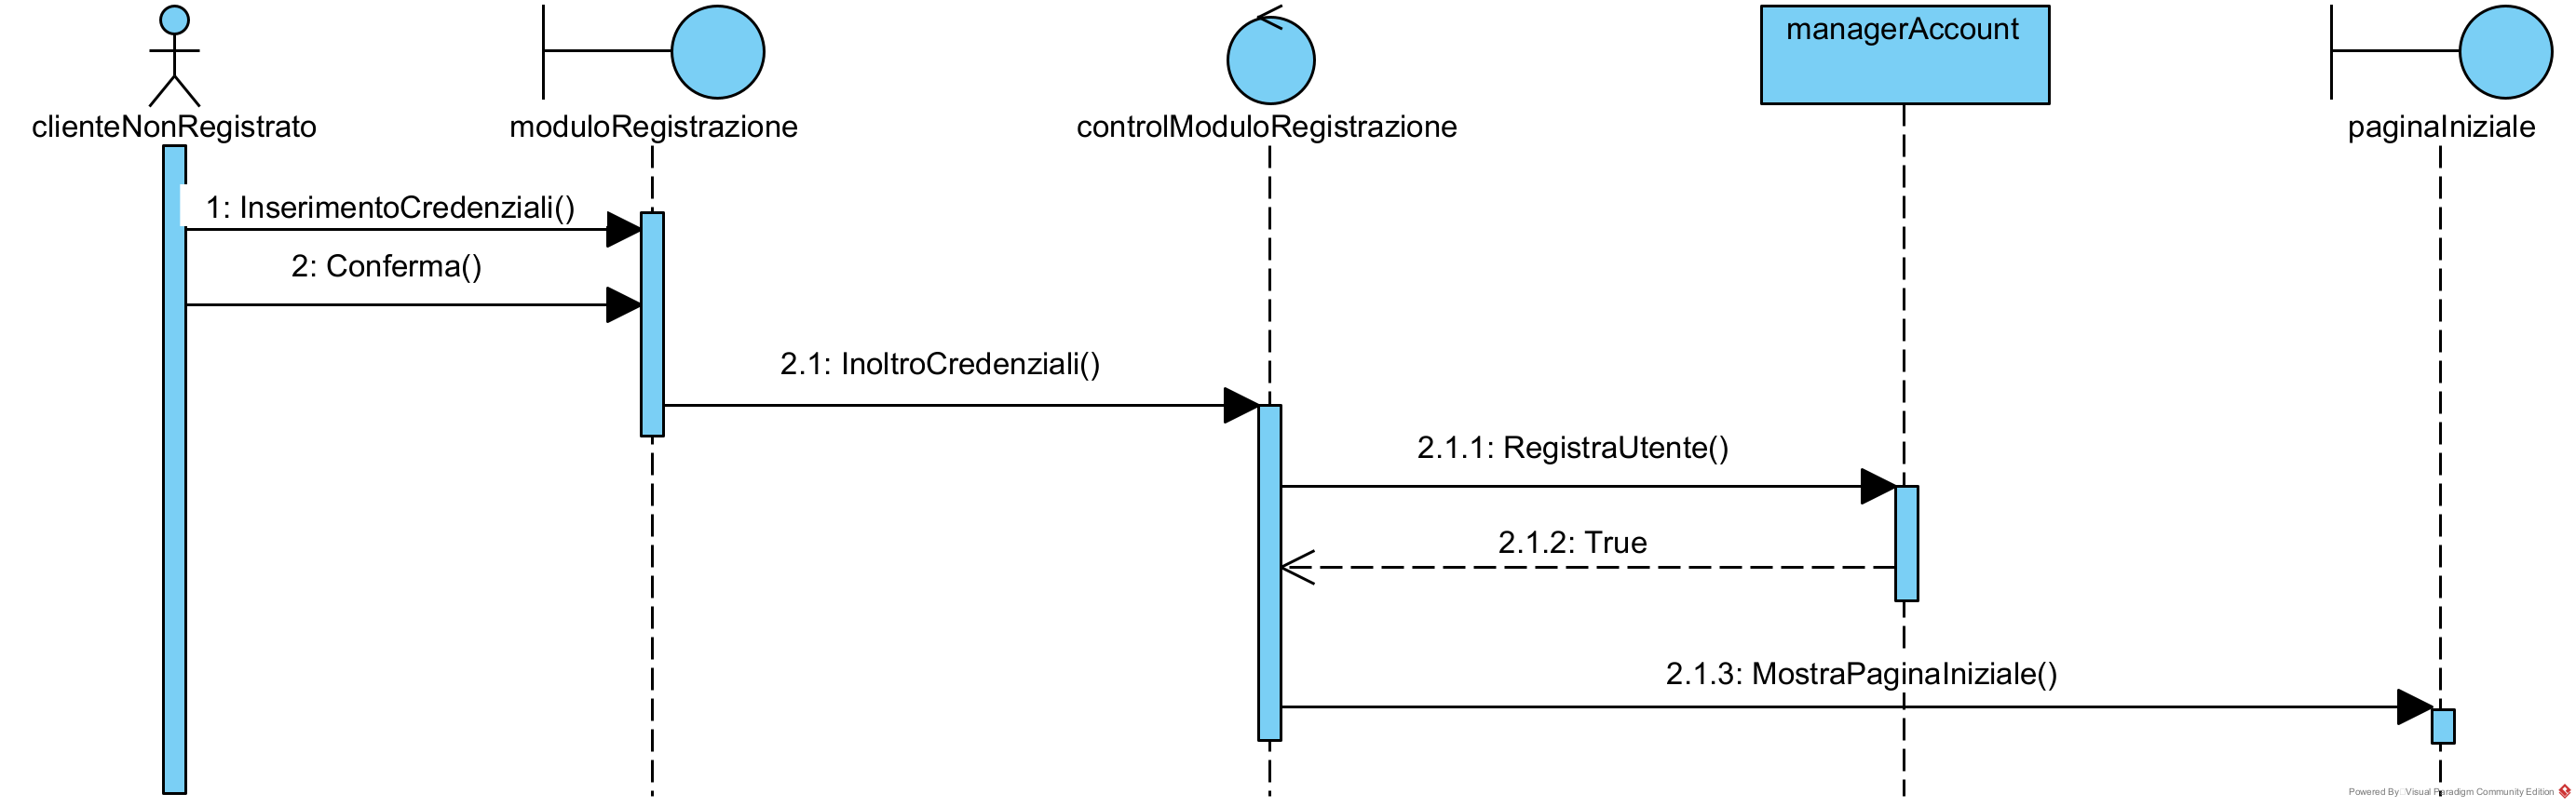
\includegraphics[width=\textwidth]{SequenceDiagram/ClienteRegistrazione}
\end{center}

\begin{enumerate}
\item Un cliente non registrato che visita il sito per la prima volta, una volta deciso di registrarsi, può fare click su ``Registrati'' dalla pagina iniziale.
\item Gli viene presentato un form in cui inserire i dati richiesti per la registrazione, tra cui nome, cognome, email e password.
\item I dati vengono controllati e, se privi di errori, l'utente viene registrato.
\end{enumerate}

\subsubsection{Cliente si autentica}
\label{SD:login}

Fare riferimento a \ref{UC:autenticazione}. \\

\begin{center}
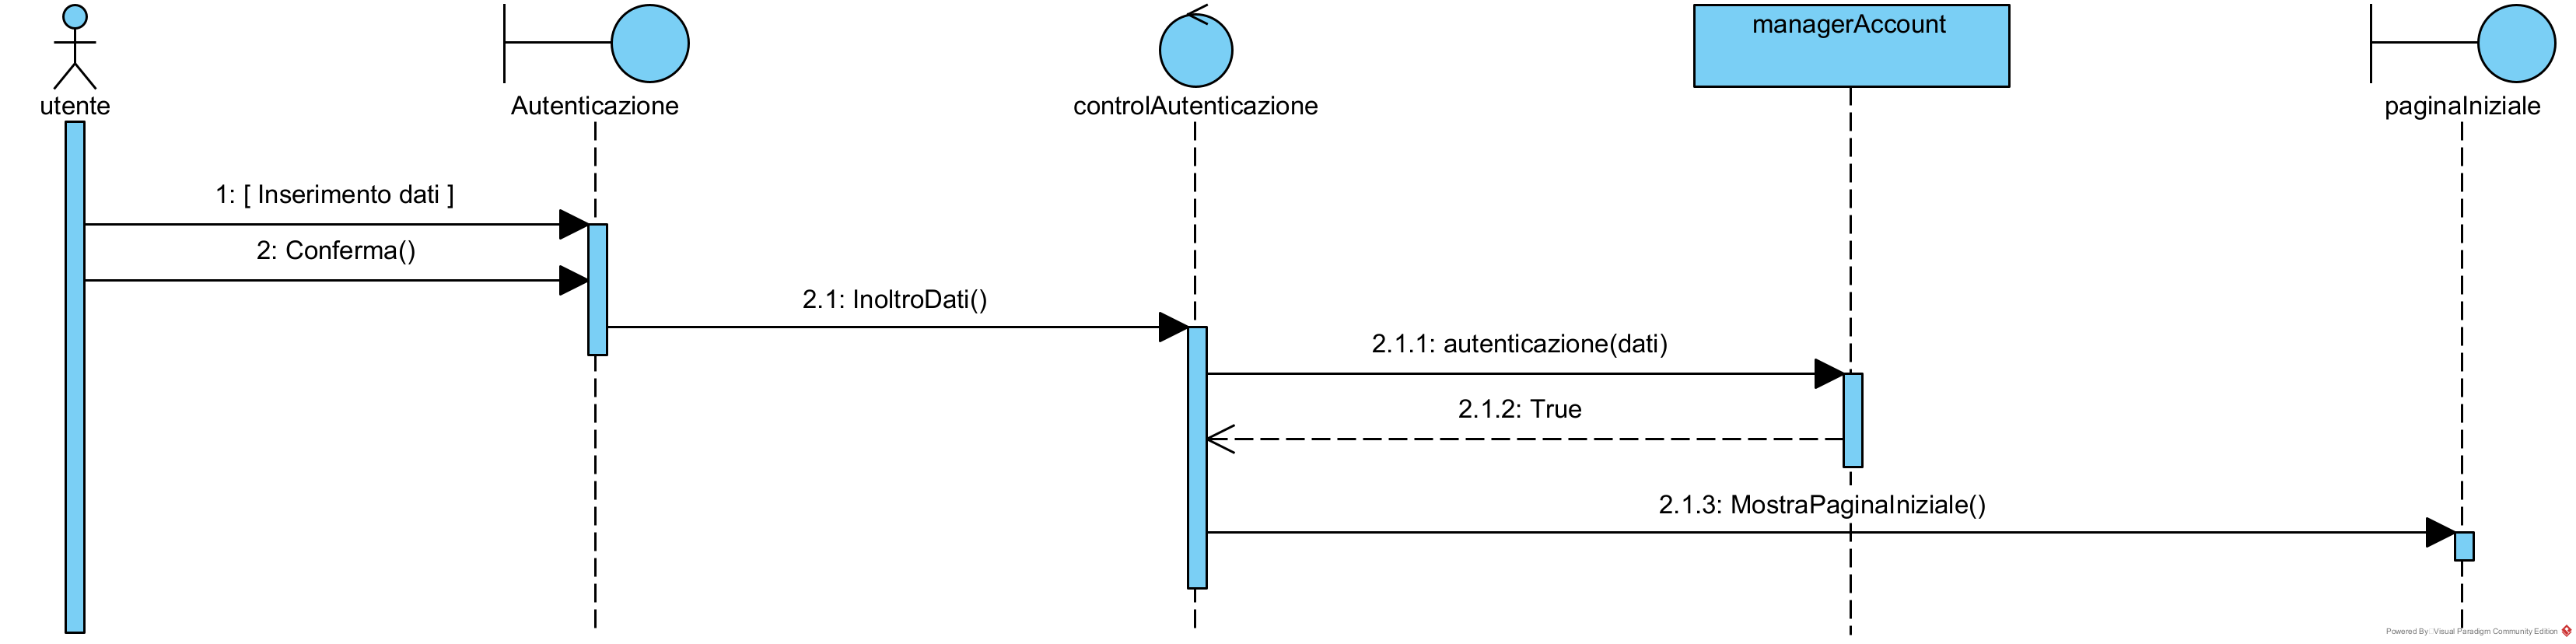
\includegraphics[width=\textwidth]{SequenceDiagram/Autenticazione}
\end{center}

\begin{enumerate}
\item Dopo la registrazione (\ref{SD:registrazione}), l'utente può usare le credenziali scelte per autenticarsi cliccando sul tasto ``Autenticati''.
\item Gli viene presentato quindi un modulo per l'inserimento di email e password.
\item Se le credenziali corrispondono a quelle memorizzate nel sistema, all'utente viene consentito l'accesso.
\end{enumerate}

\subsubsection{Cliente ricerca un articolo}
\label{SD:ricerca}

\begin{center}
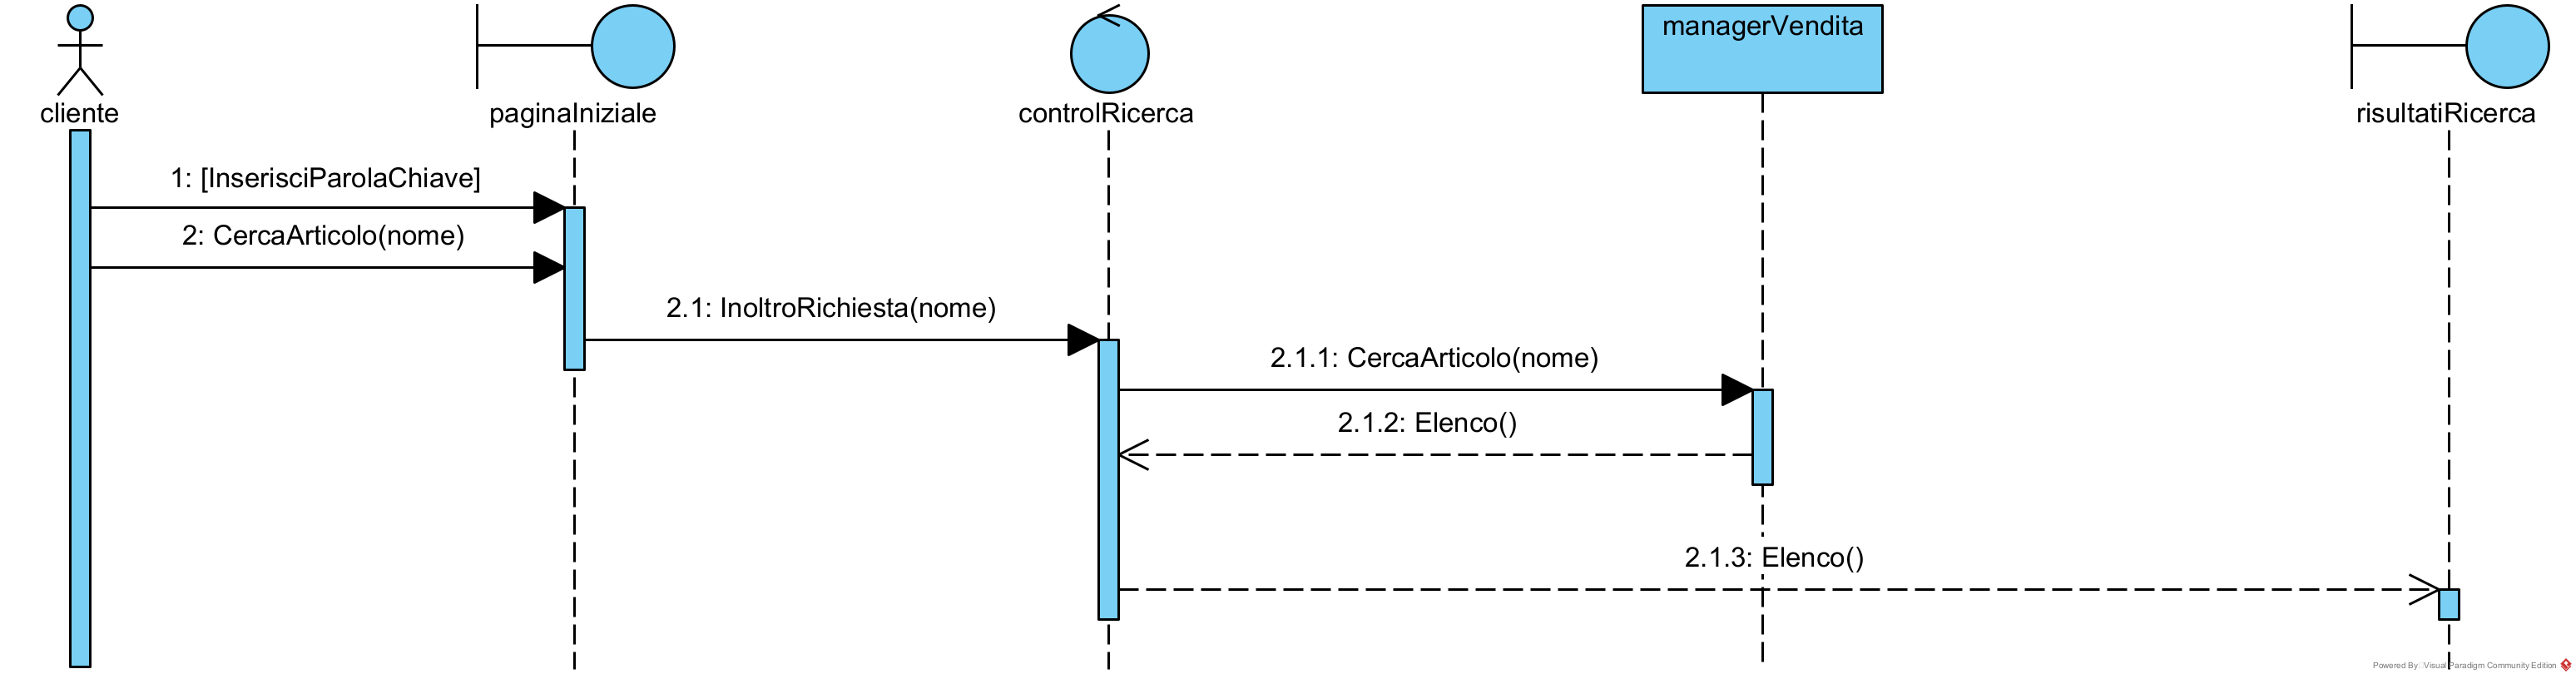
\includegraphics[width=\textwidth]{SequenceDiagram/ClienteArticoloRicerca}
\end{center}

\begin{enumerate}
\item Ai clienti e agli utenti non autenticati è permesso ricercare articoli nel sito. Usando la barra di ricerca presente nella pagina iniziale, può inserire dei termini da ricercare.
\item Una volta premuto sul tasto ``Cerca'', gli viene presentato un elenco di articoli corrispondenti.
\end{enumerate}

\subsubsection{Cliente visualizza dettagli di un articolo}
\label{SD:dettagli}

\begin{center}
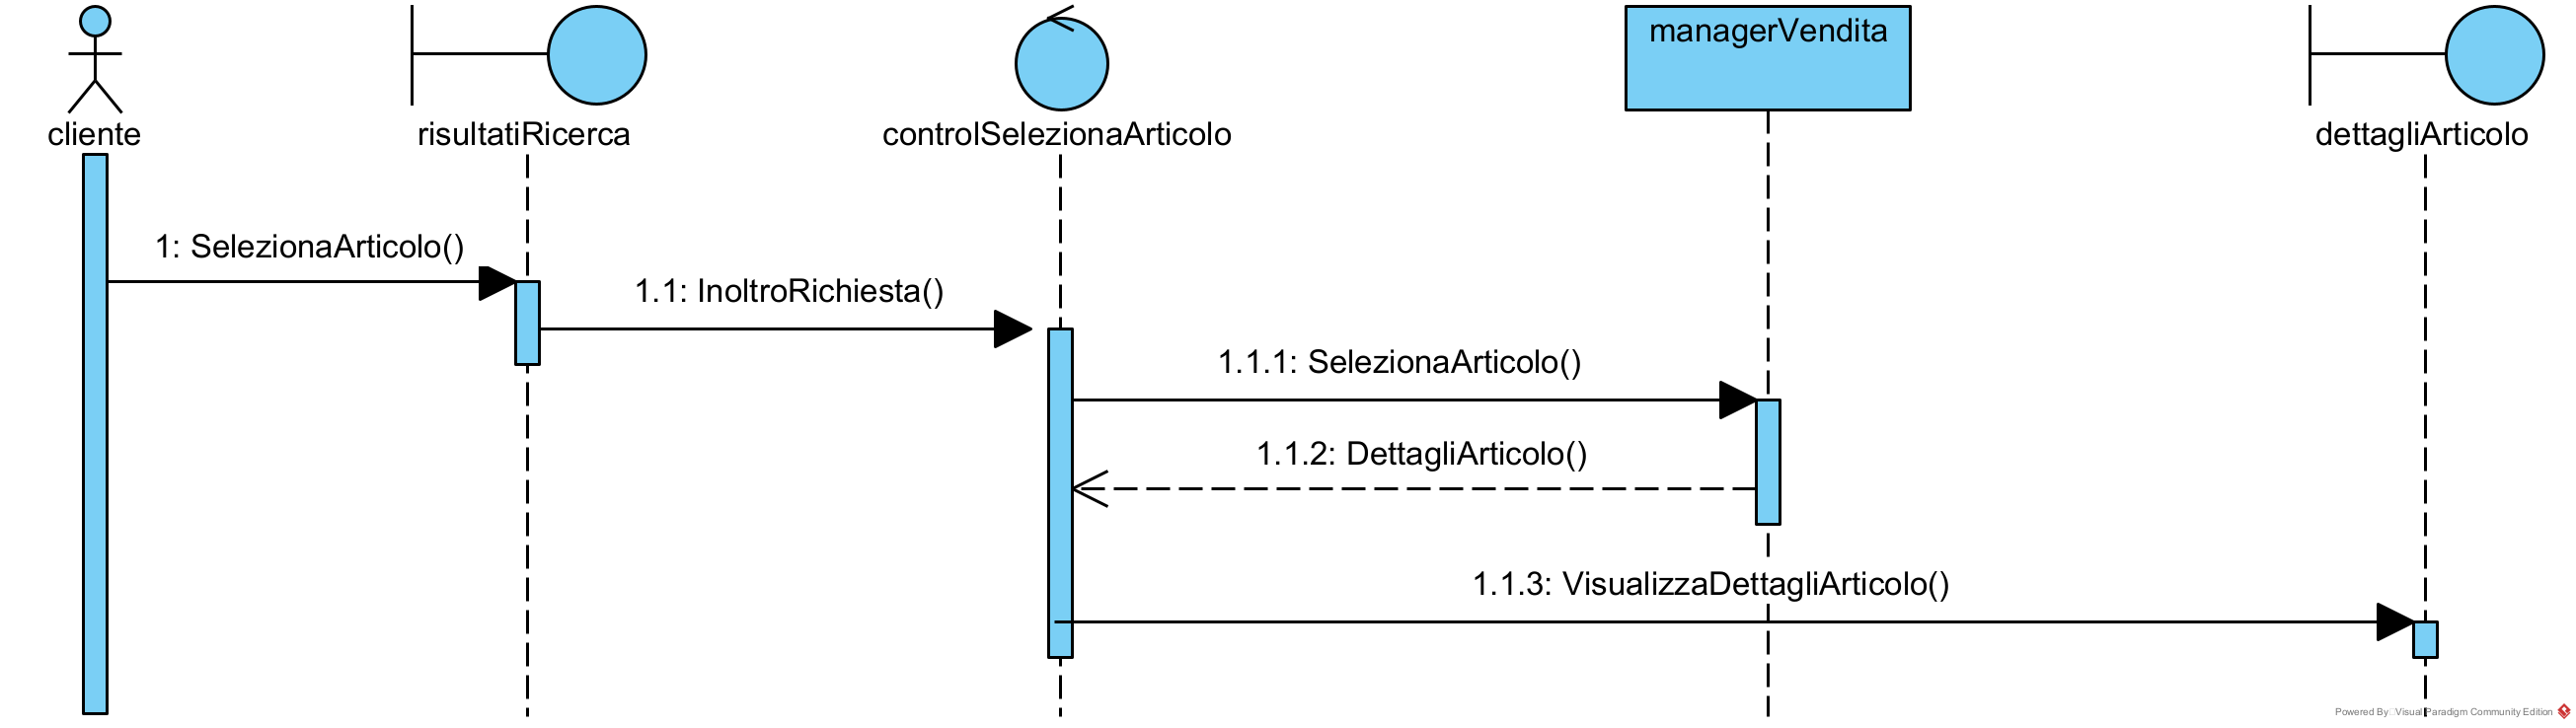
\includegraphics[width=\textwidth]{SequenceDiagram/ClienteArticoloSeleziona}
\end{center}

\begin{enumerate}
\item Dopo aver effettuato una ricerca (\ref{SD:ricerca}), un utente può scegliere uno degli articoli e selezionarlo per visualizzarne i dettagli.
\item All'utente viene presentata una pagina con i dettagli dell'articolo scelto.
\end{enumerate}

\newpage

\subsubsection{Cliente aggiunge un articolo al carrello}
\label{SD:aggiunta}

Fare riferimento a \ref{UC:carrelloadd}. \\

\begin{center}
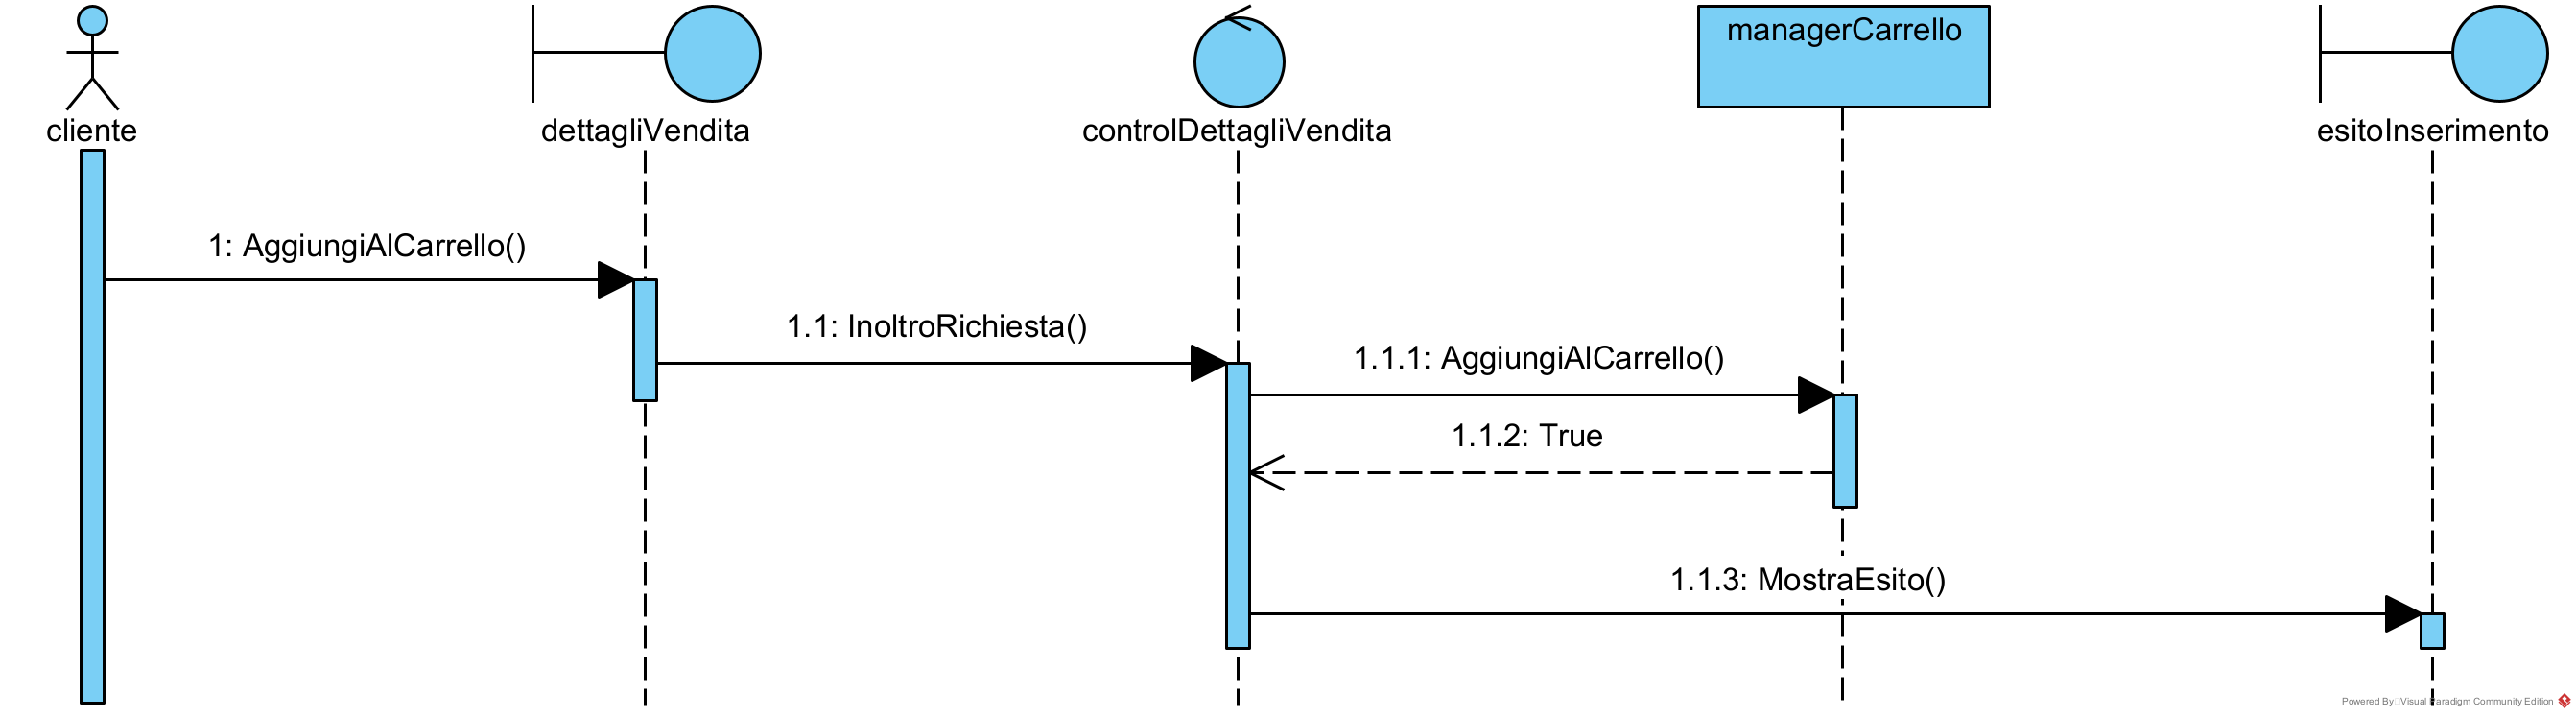
\includegraphics[width=\textwidth]{SequenceDiagram/ClienteCarrelloAggiunge}
\end{center}

\begin{enumerate}
\item Dopo essersi autenticato (\ref{SD:login}) e aver selezionato un articolo (\ref{SD:dettagli}) può aggiungere un articolo al carrello utilizzando il tasto ``Aggiungi al carrello". Se non è autenticato, gli verrà chiesto di farlo.

\item Una volta premuto, la sua aggiunta viene registrata nel sistema per mantenere il carrello attraverso browser e dispositivi diversi e all'utente viene mostrata una pagina di conferma.
\end{enumerate}

\subsubsection{Cliente rimuove un articolo dal carrello}
\label{SD:rimozione}

Fare riferimento a \ref{UC:carrelloremove}. \\

\begin{center}
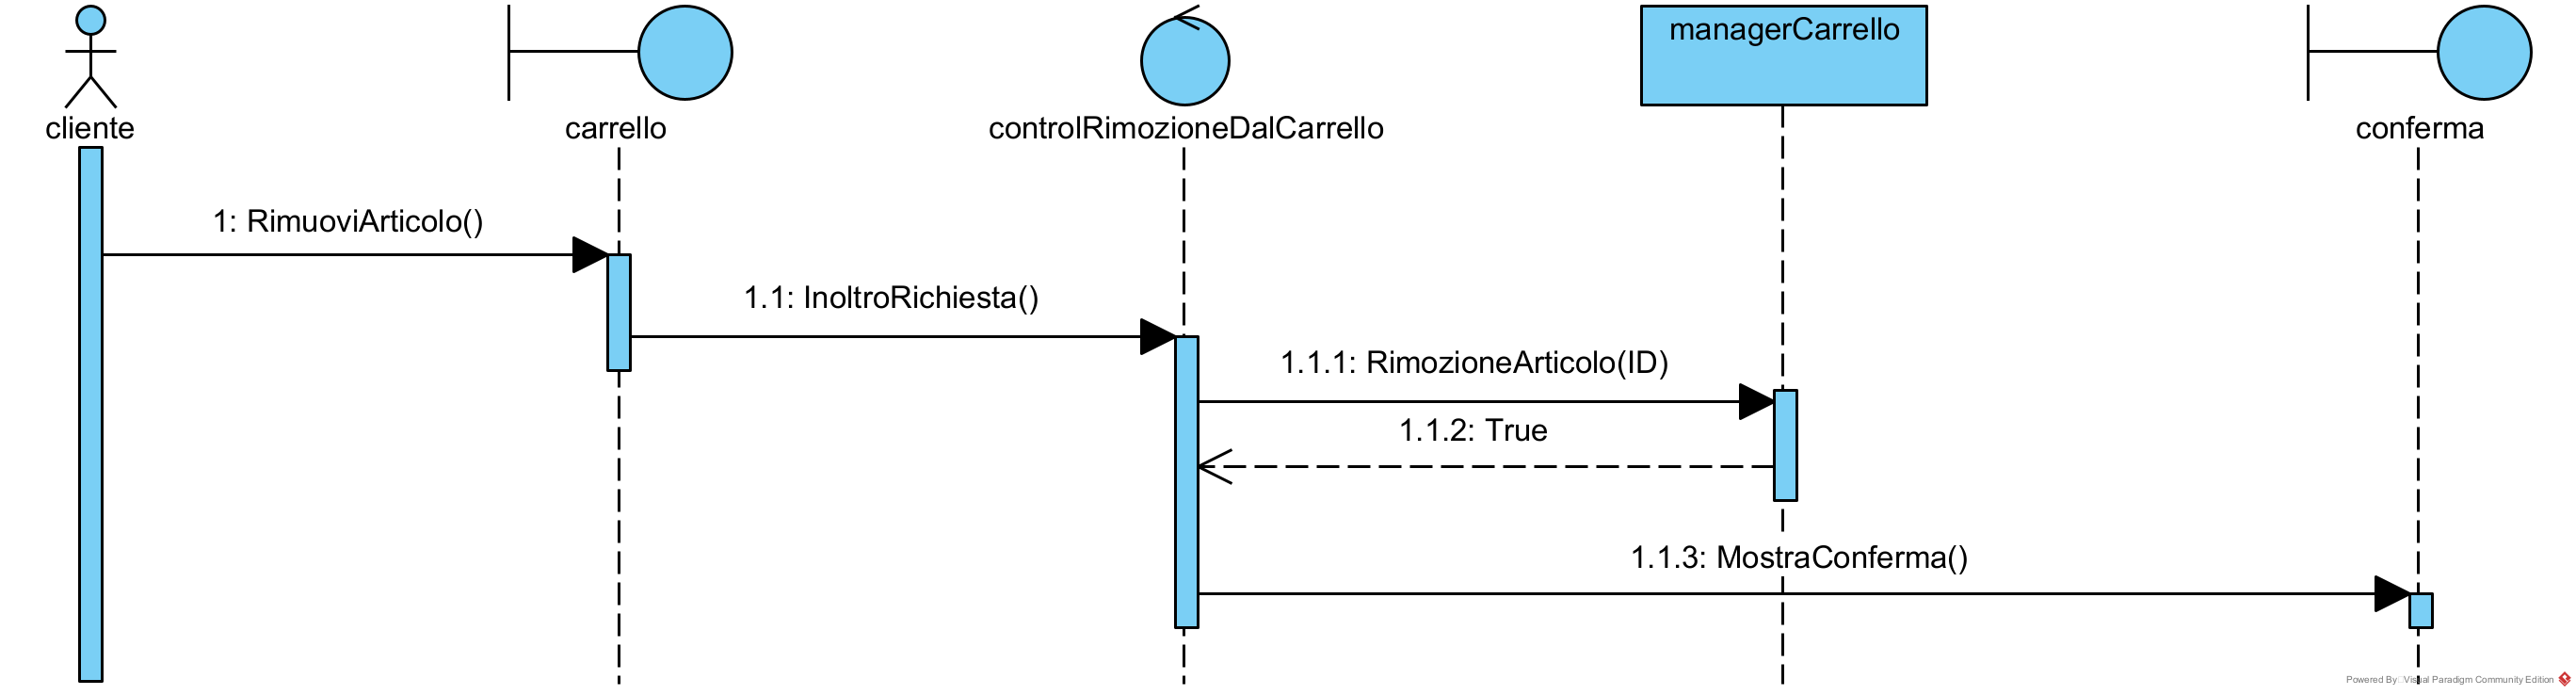
\includegraphics[width=\textwidth]{SequenceDiagram/ClienteCarrelloRimuove}
\end{center}

\begin{enumerate}
\item Dopo aver aggiunto un articolo al carrello (\ref{SD:aggiunta}), all'utente è consentita la rimozione degli articoli dal carrello usando il tasto ``Rimuovi".
\item Una volta premuto, la sua modifica viene registrata e all'utente viene mostrata una pagina di conferma.
\end{enumerate}

\newpage

\subsubsection{Cliente acquista articoli}
\label{SD:acquista}

\begin{center}
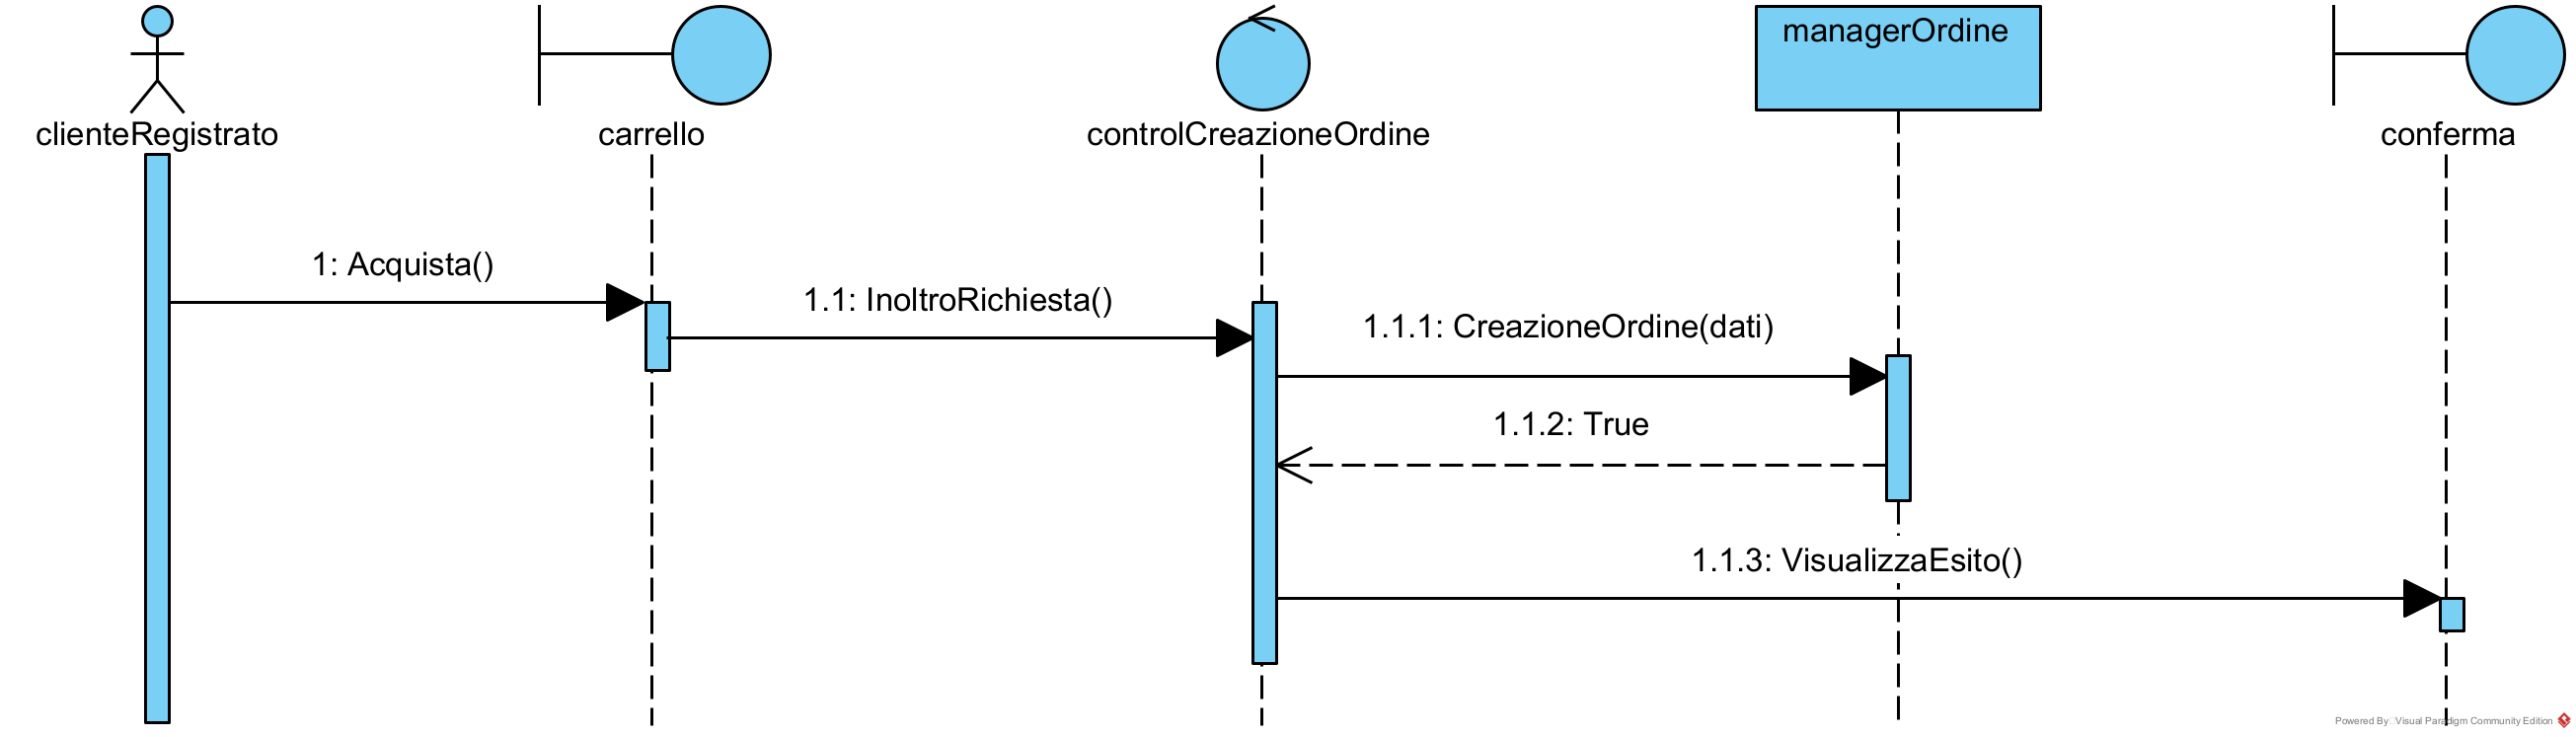
\includegraphics[width=\textwidth]{SequenceDiagram/ClienteArticoloAcquista}
\end{center}

\begin{enumerate}
\item Dopo aver aggiunto almeno un articolo al carrello (\ref{SD:aggiunta}), l'utente ha la possibilità di ordinare gli articoli nel carrello stesso.
\item Dopo aver premuto su ``Acquista'', l'ordine viene registrato ed è visualizzabile da un magazziniere (\ref{SD:magazzinierespedisce}).
\end{enumerate}

\subsubsection{Cliente visualizza storico ordini}
\label{SD:storicoordini}
\begin{center}
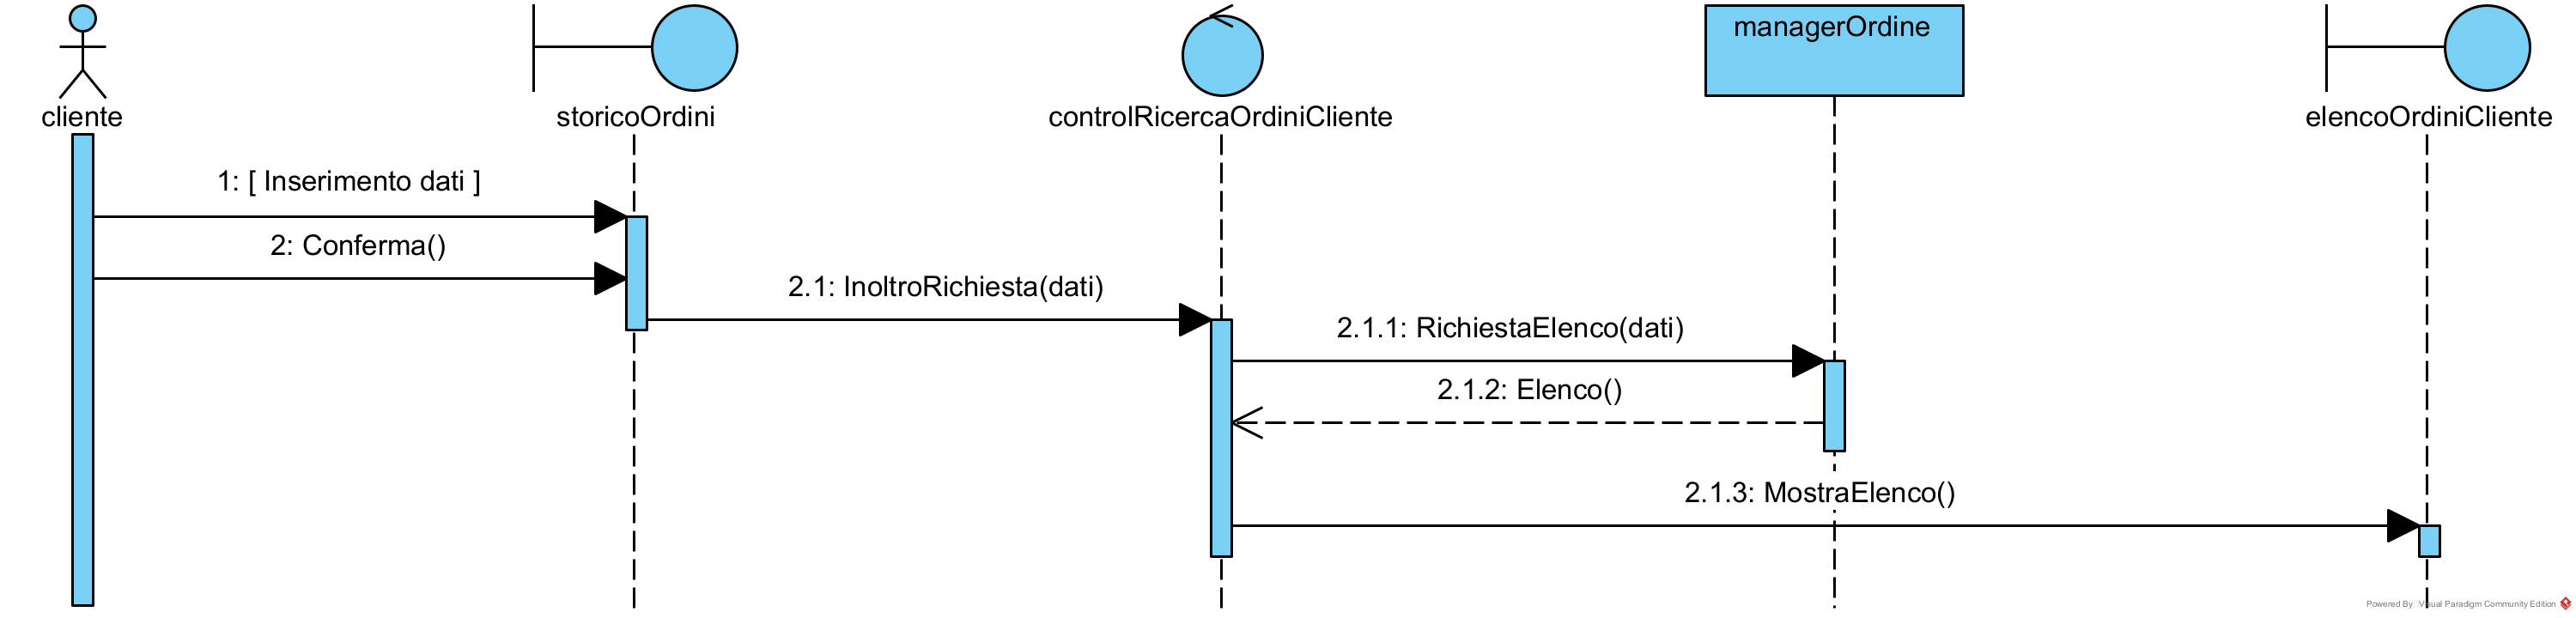
\includegraphics[width=\textwidth]{SequenceDiagram/ClienteOrdiniRicerca}
\end{center}

\begin{enumerate}
\item Se un cliente vuole visualizzare lo storico dei suoi ordini, può farlo usando il tasto ``Storico ordini" dalla pagina iniziale.
\item Inserendo una o più parole chiave nella barra di ricerca che gli viene presentata può visualizzare un elenco di ordini corrispondenti.
\end{enumerate}

\newpage

\subsubsection{Cliente annulla ordine}
\label{SD:annull}

Fare riferimento a \ref{UC:annullamento}. \\

\begin{center}
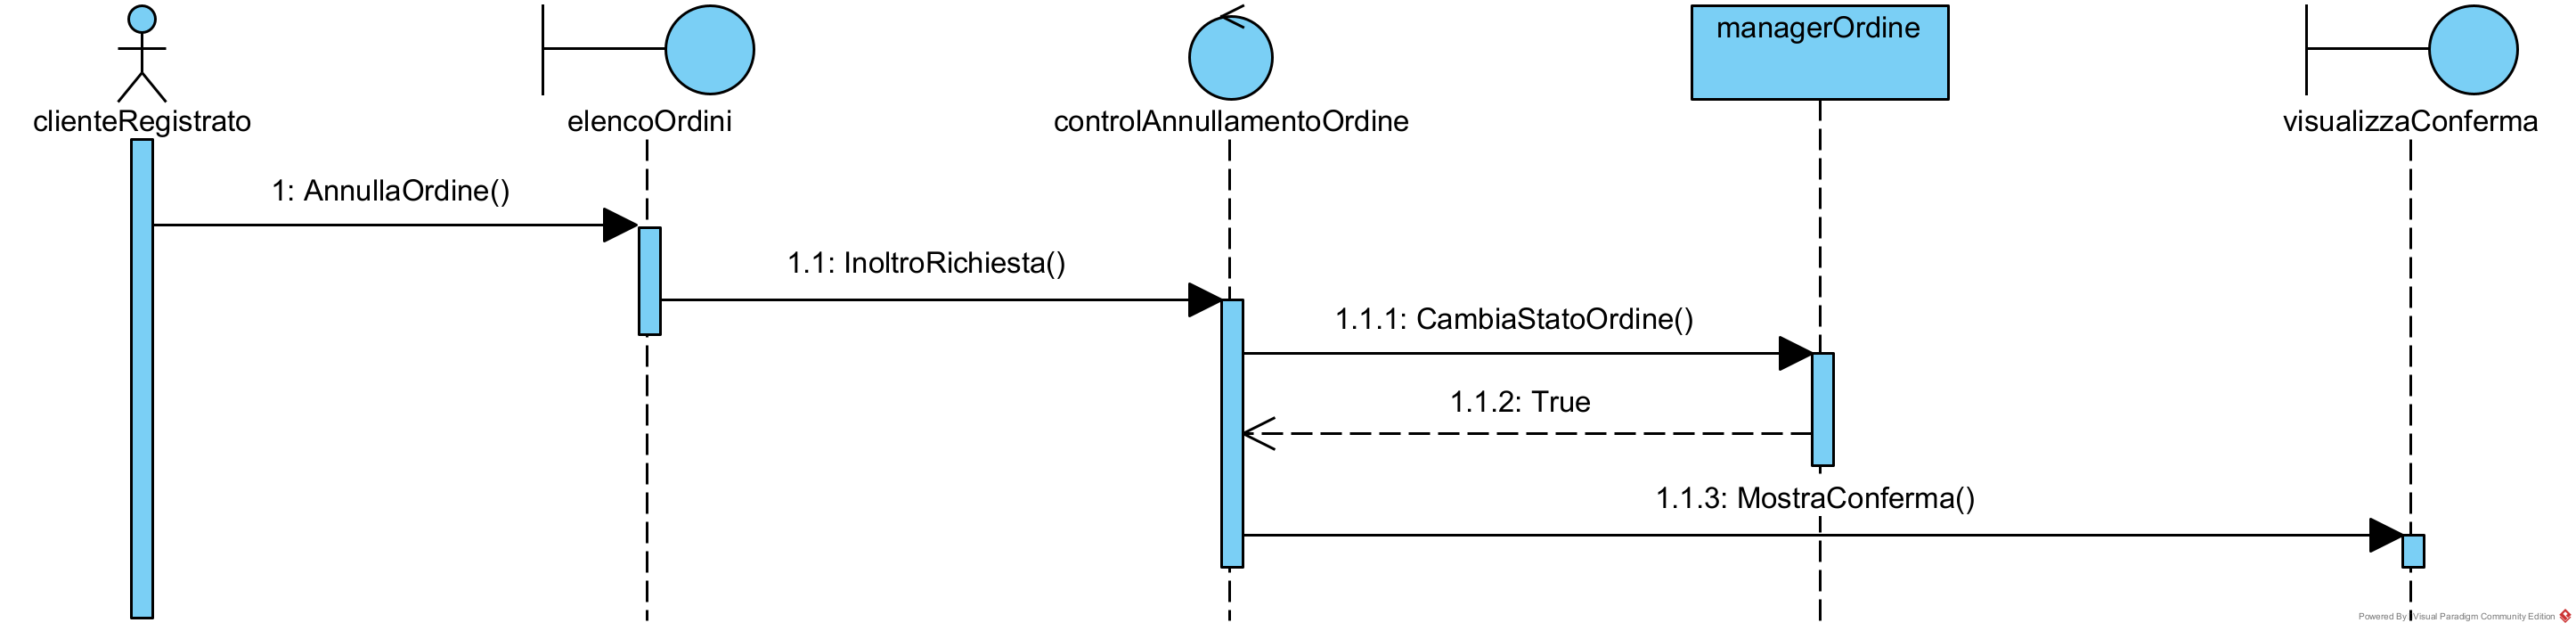
\includegraphics[width=\textwidth]{SequenceDiagram/ClienteOrdineAnnulla}
\end{center}

\begin{enumerate}
\item Dopo aver effettuato un ordine e prima che venga spedito, ad un cliente è permesso annullare un ordine.
\item Dall'elenco degli ordini ha la possibilità di richiedere l'annullamento. Se lo stato nel sistema è ancora ``InAttesa'' l'ordine viene effettivamente annullato immediatamente e non sarà più visualizzabile dai magazzinieri (\ref{SD:magazzinierespedisce}). In caso contrario, non è possibile annullarlo.
\end{enumerate}

\newpage

\subsubsection{Cliente visualizza elenco vendite}
\label{SD:elencovendite}

\begin{center}
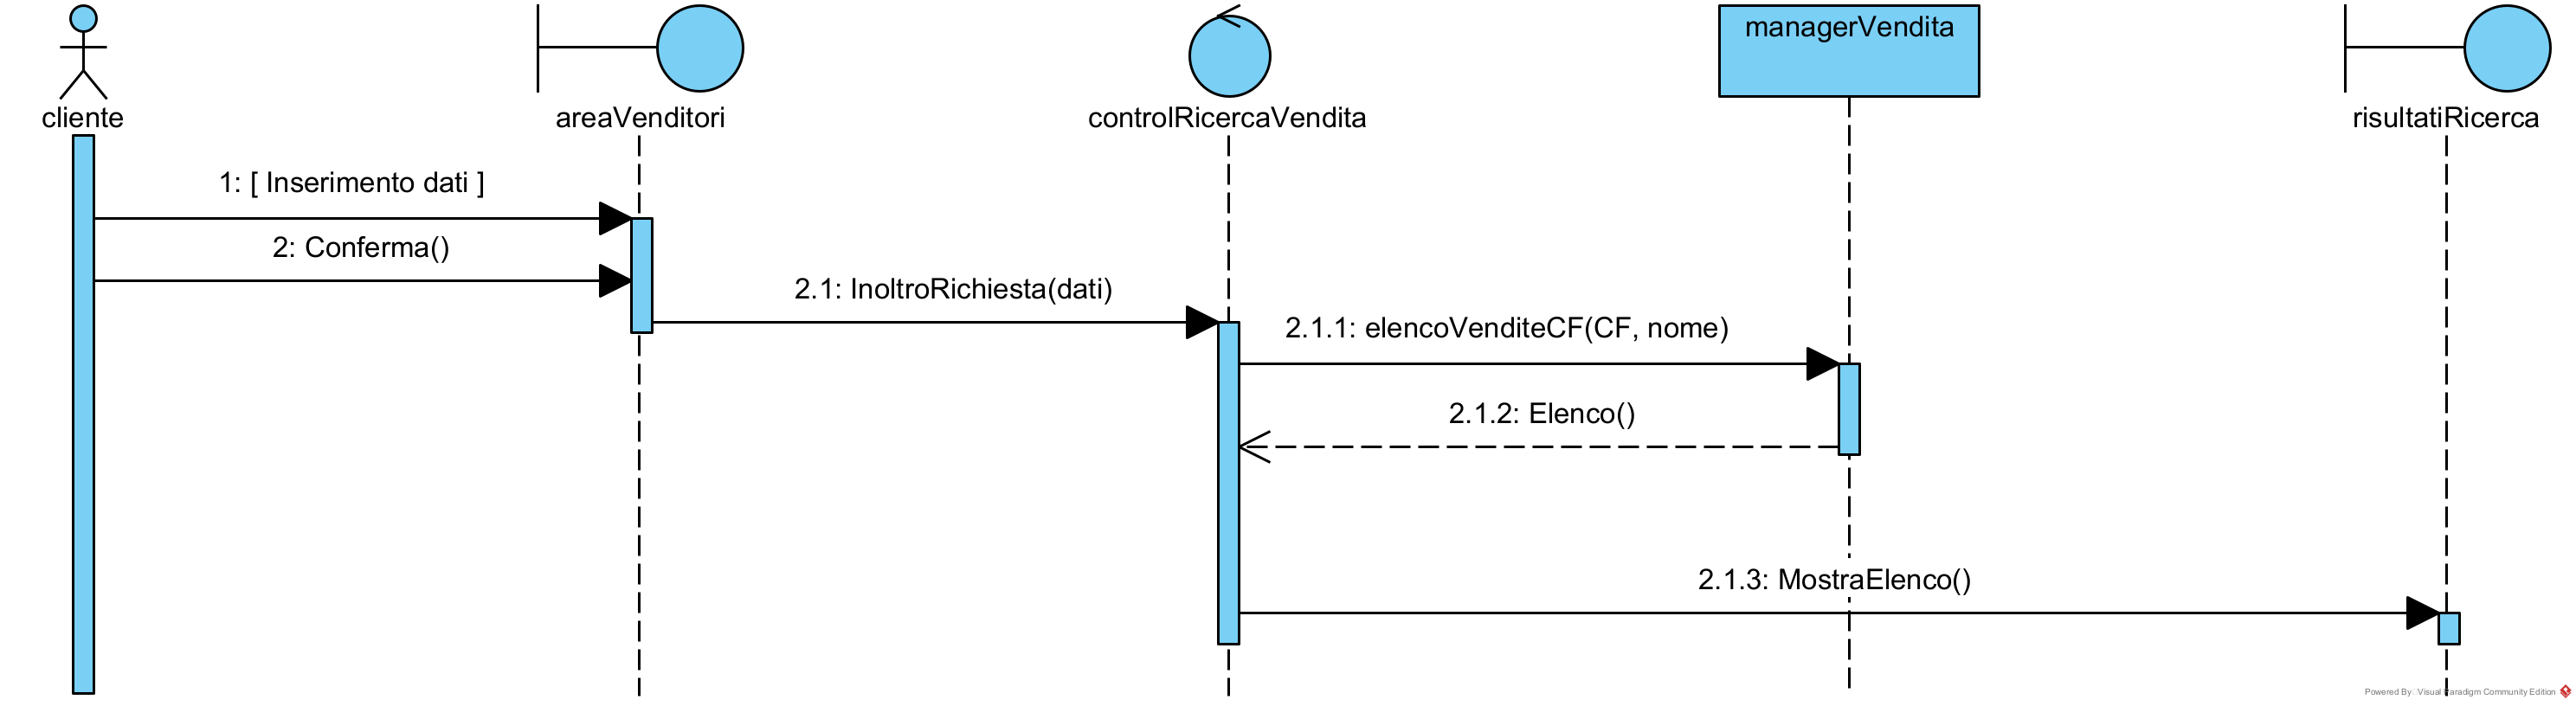
\includegraphics[width=\textwidth]{SequenceDiagram/ClienteVenditaRicerca}
\end{center}

\begin{enumerate}
\item Dalla pagina iniziale, l'utente può selezionare la voce ``Area venditori" per visualizzare la pagina dedicata alla gestione delle vendite.
\item Al caricamento della pagina, vengono caricate le vendite create più recentemente, ovvero nei 60 giorni precedenti.
\end{enumerate}

\subsubsection{Cliente vende articolo}
\label{SD:creazionevendita}

Fare riferimento a \ref{UC:salesnew}. \\

\begin{center}
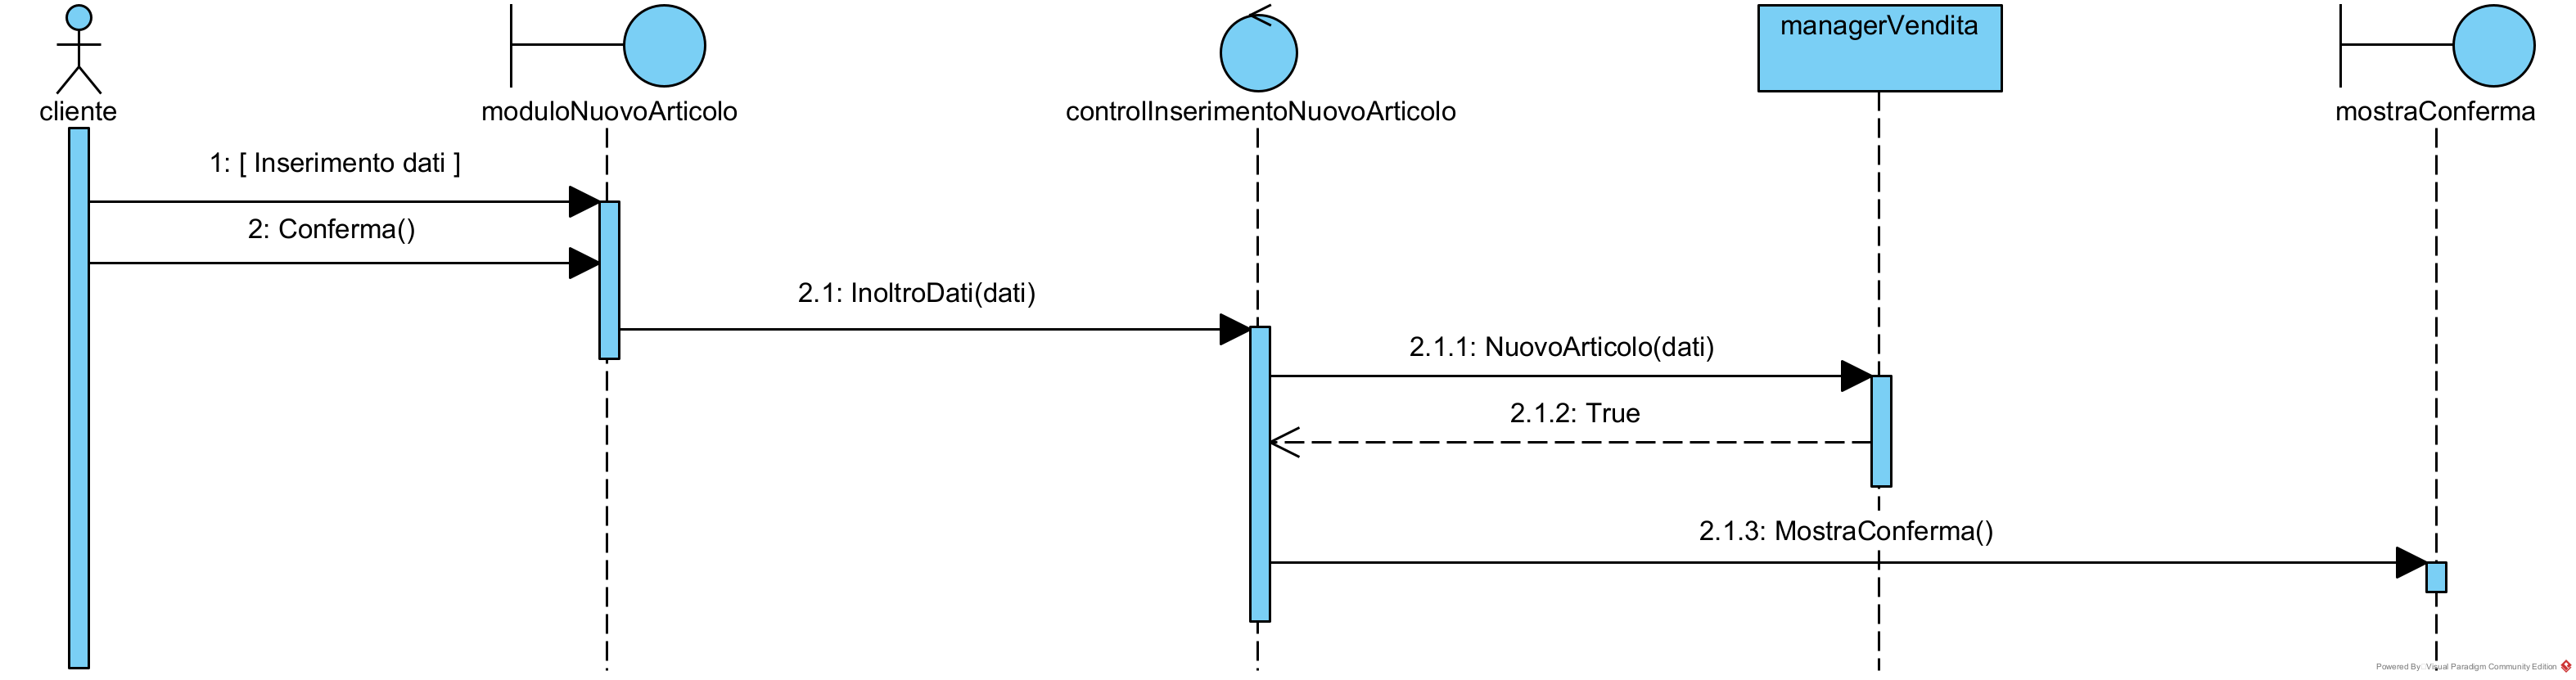
\includegraphics[width=\textwidth]{SequenceDiagram/ClienteVenditaCrea}
\end{center}

\begin{enumerate}
\item Dall'elenco delle vendite (\ref{SD:elencovendite}), è sufficiente utilizzare il tasto ``Inserisci nuova vendita".
\item Viene richiesto all'utente di compilare un modulo con i dati necessari come nome, prezzo, descrizione, quantità disponibile e di inserire almeno 3 foto del prodotto.
\item La nuova vendita viene quindi inserita nel sistema in uno stato di attesa finché un centralinista non verificherà le informazioni della vendita (\ref{SD:centralinistaautorizza}).
\end{enumerate}

\subsubsection{Cliente seleziona vendita}
\label{SD:selezionavenditacliente}

\begin{center}
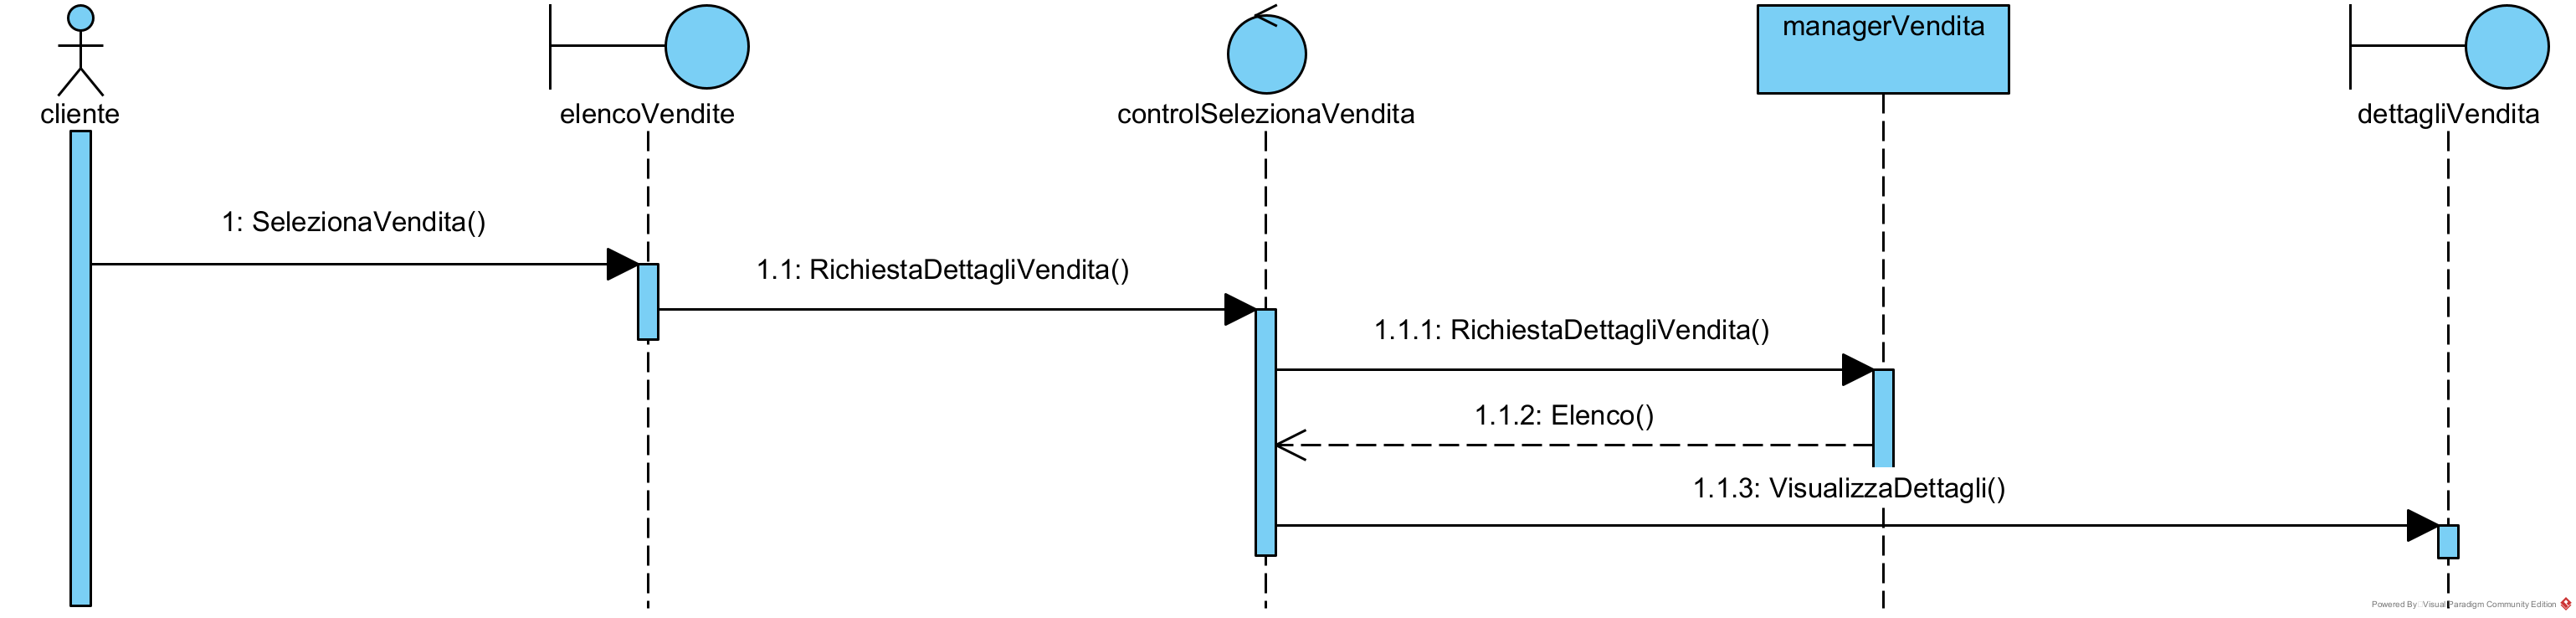
\includegraphics[width=\textwidth]{SequenceDiagram/ClienteVenditaSeleziona}
\end{center}

\begin{enumerate}
\item Dai risultati di ricerca per le vendite (\ref{SD:elencovendite}), il cliente ne può selezionare una per visualizzarne i dettagli.
\item Gli viene mostrata una pagina con informazioni sulla vendita come la quantità di articoli venduti e il ricavato totale.
\end{enumerate}

\subsubsection{Cliente modifica vendita}
\label{SD:modificavendita}

\begin{center}
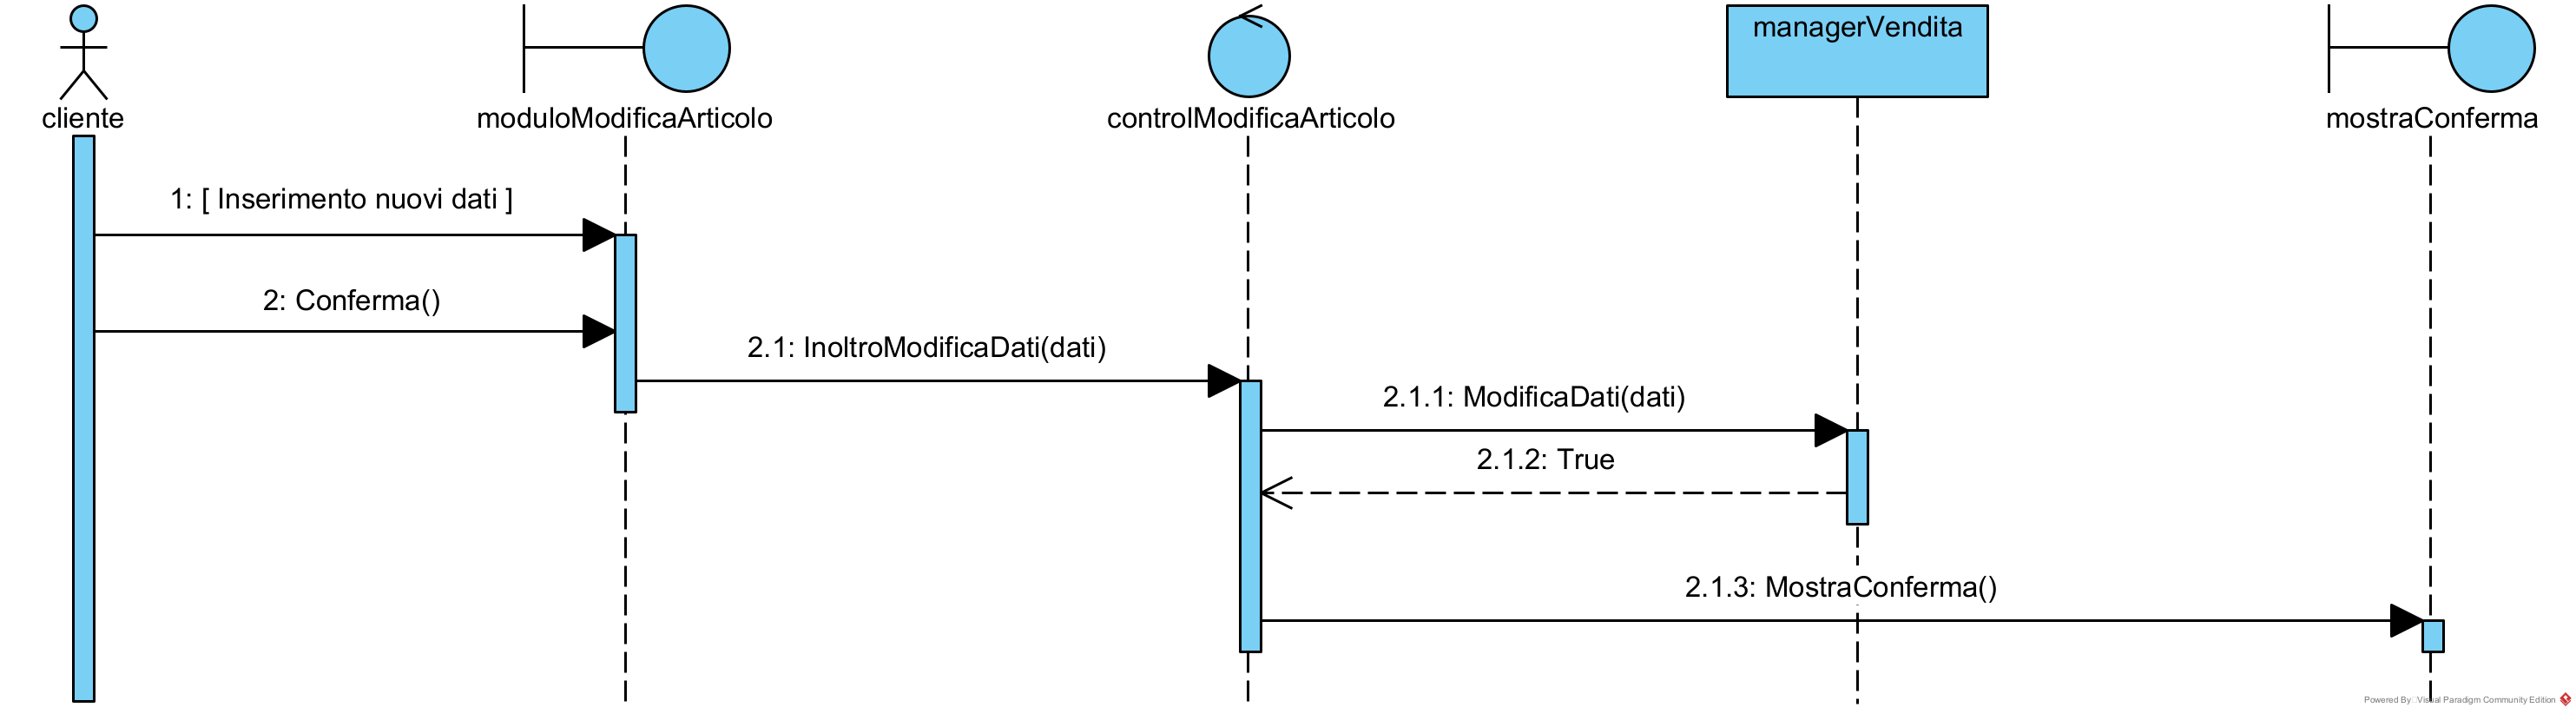
\includegraphics[width=\textwidth]{SequenceDiagram/ClienteVenditaModifica}
\end{center}

\begin{enumerate}
\item Nella pagina dei dettagli di una vendita, se lo stato è ``In vendita", è presente anche un tasto ``Modifica vendita".
\item L'utente può cliccarlo per visualizzare un modulo per la modifica della vendita. 
\item La vendita torna quindi in uno stato di attesa finché un centralinista non verificherà i dati inseriti (\ref{SD:centralinistaautorizza}).
\end{enumerate}

\newpage

\subsubsection{Cliente annulla vendita}
\label{SD:annullavendita}

\begin{center}
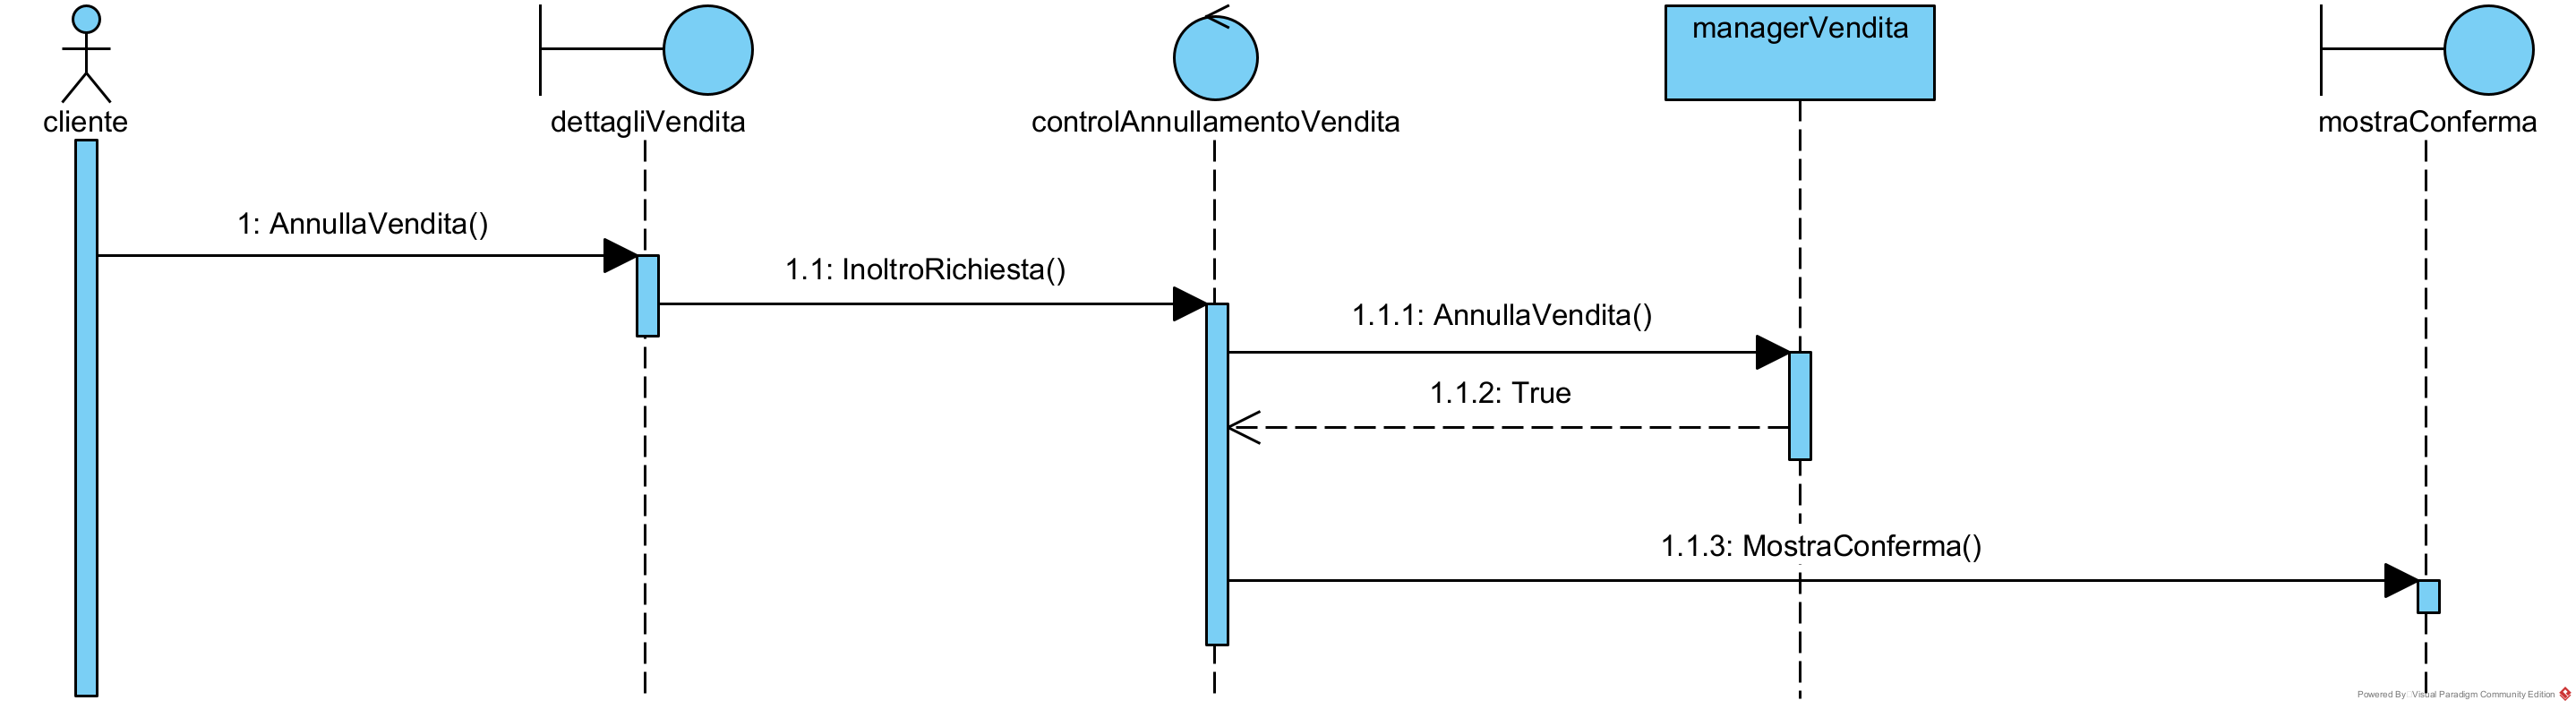
\includegraphics[width=\textwidth]{SequenceDiagram/ClienteVenditaAnnulla}
\end{center}

\begin{enumerate}
\item Dopo aver creato una vendita (\ref{SD:creazionevendita}) e finché lo stato è ``In vendita", all'utente è concessa la possibilità di annullare una vendita.
\item Dall'elenco delle vendite è presente quindi un tasto ``Annulla vendita".
\item All'utente viene mostrata una pagina di conferma.
\end{enumerate}

\newpage

\subsubsection{Cliente elenca ticket}
\label{SD:elencoticket}
Fare riferimento a \ref{UC:ticketlist}. \\

\begin{center}
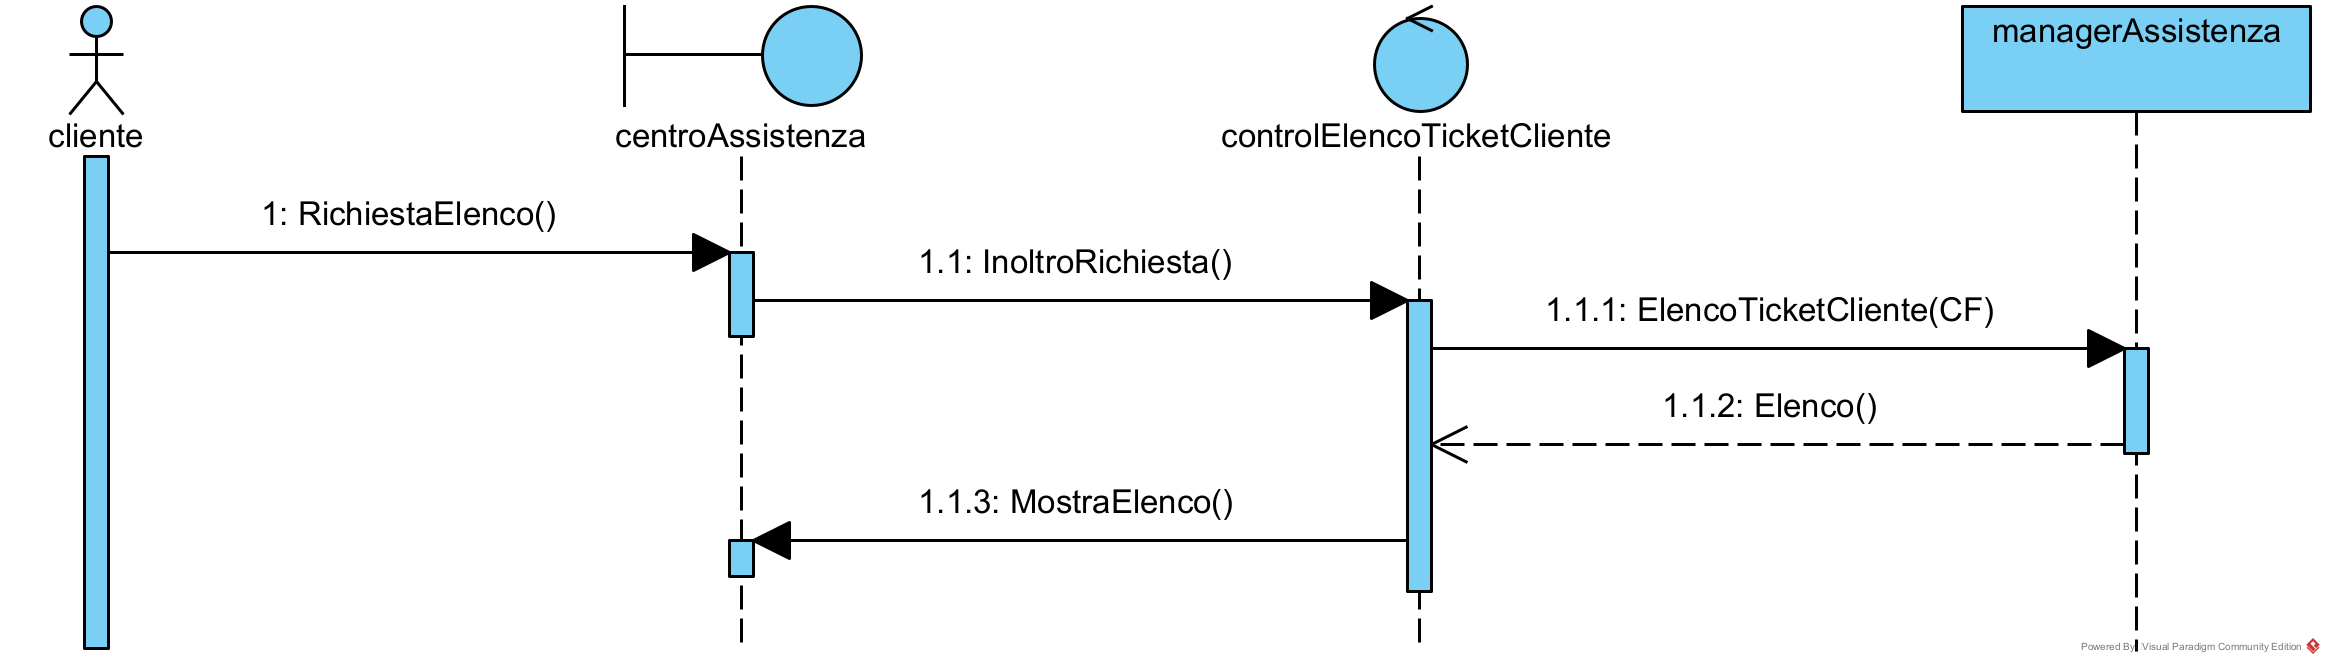
\includegraphics[width=\textwidth]{SequenceDiagram/ClienteTicketElenco}
\end{center}

\begin{enumerate}
\item Un utente autenticato (\ref{SD:login}) che si trova nella pagina iniziale può utilizzare la funzione ``Assistenza Clienti".
\item Gli viene quindi mostrato l'elenco dei ticket attualmente in attesa di risoluzione e che non sono attualmente visualizzati da altri centralinisti.
\end{enumerate}

\subsubsection{Cliente apre ticket}
\label{SD:aperturaticket}

\begin{center}
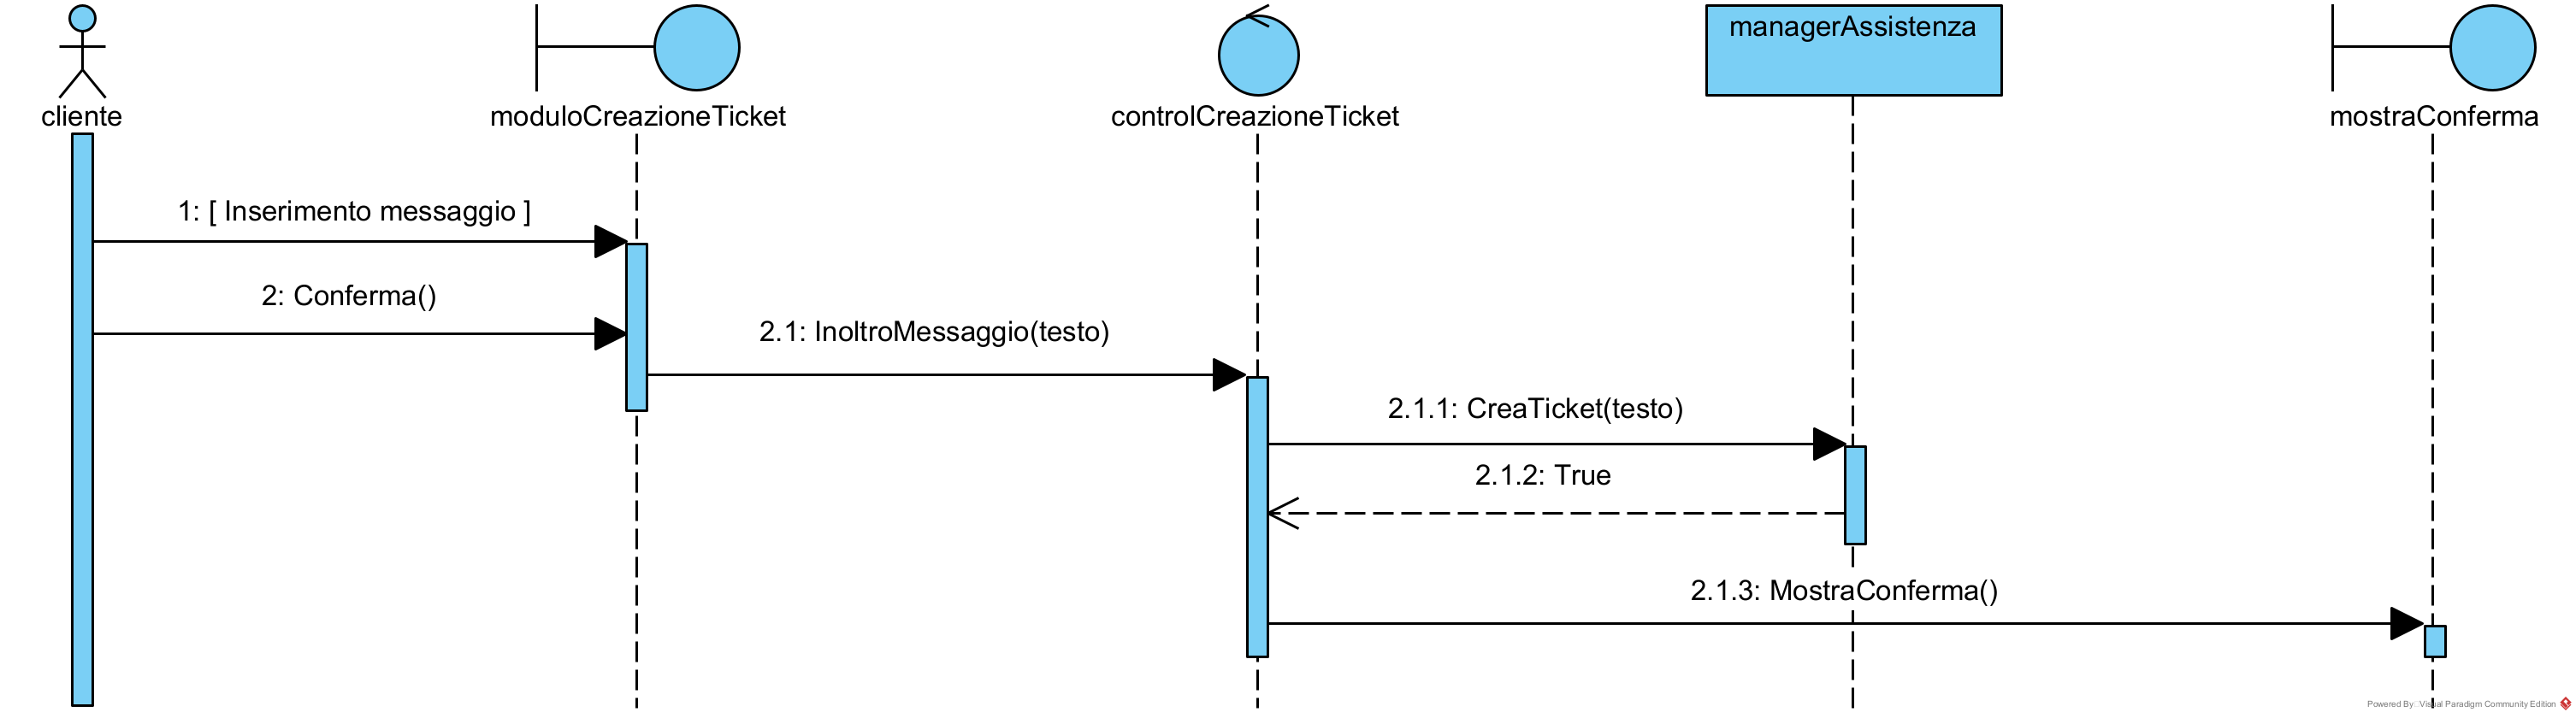
\includegraphics[clip,width=\textwidth]{SequenceDiagram/ClienteTicketCreazione}
\end{center}

\begin{enumerate}
\item Dall'elenco dei ticket (\ref{SD:elencoticket}), l'utente usa la funzione ``Crea Ticket".
\item Gli viene mostrato un modulo per l'inserimento del messaggio per la scelta della tipologia del problema.
\item All'utente viene mostrata una conferma.
\end{enumerate}

\newpage

\subsubsection{Cliente seleziona un ticket}
\label{SD:selezioneticketcliente}

\begin{center}
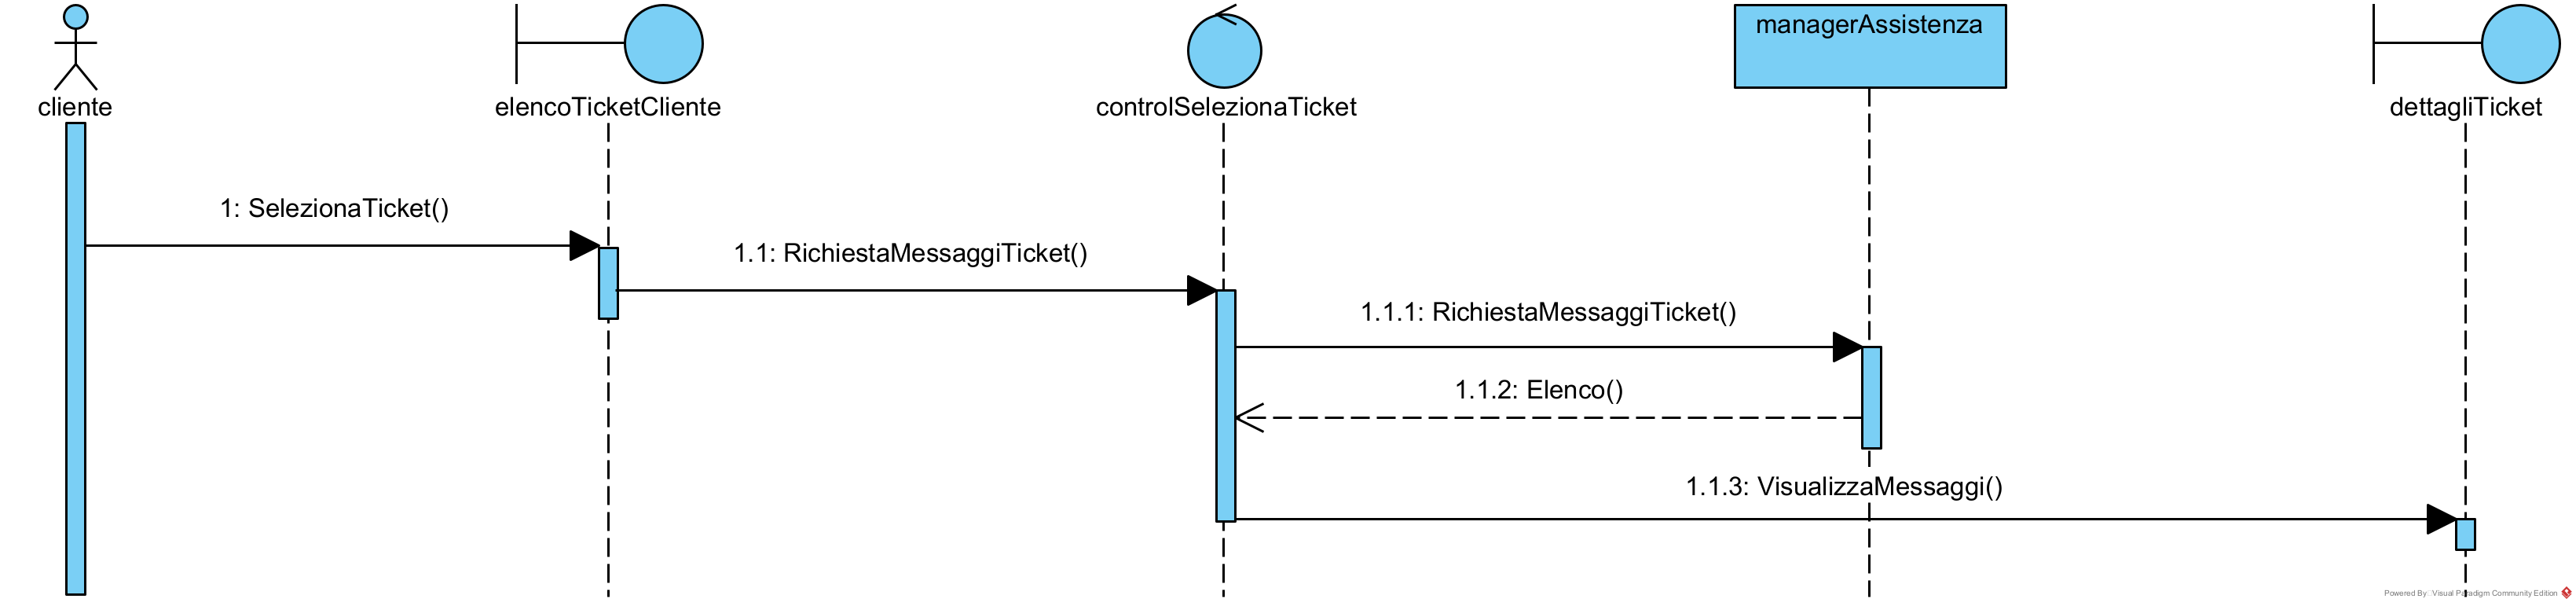
\includegraphics[width=\textwidth]{SequenceDiagram/ClienteTicketSeleziona}
\end{center}

\begin{enumerate}
\item Dall'elenco dei ticket (\ref{SD:elencoticket}), l'utente fa click su uno dei ticket attualmente aperti.
\item Gli vengono mostrati tutti i messaggi inviati fino a quel momento.
\end{enumerate}

\newpage

\subsubsection{Cliente risponde ad un ticket}
\label{SD:rispostaticketcliente}

\begin{center}
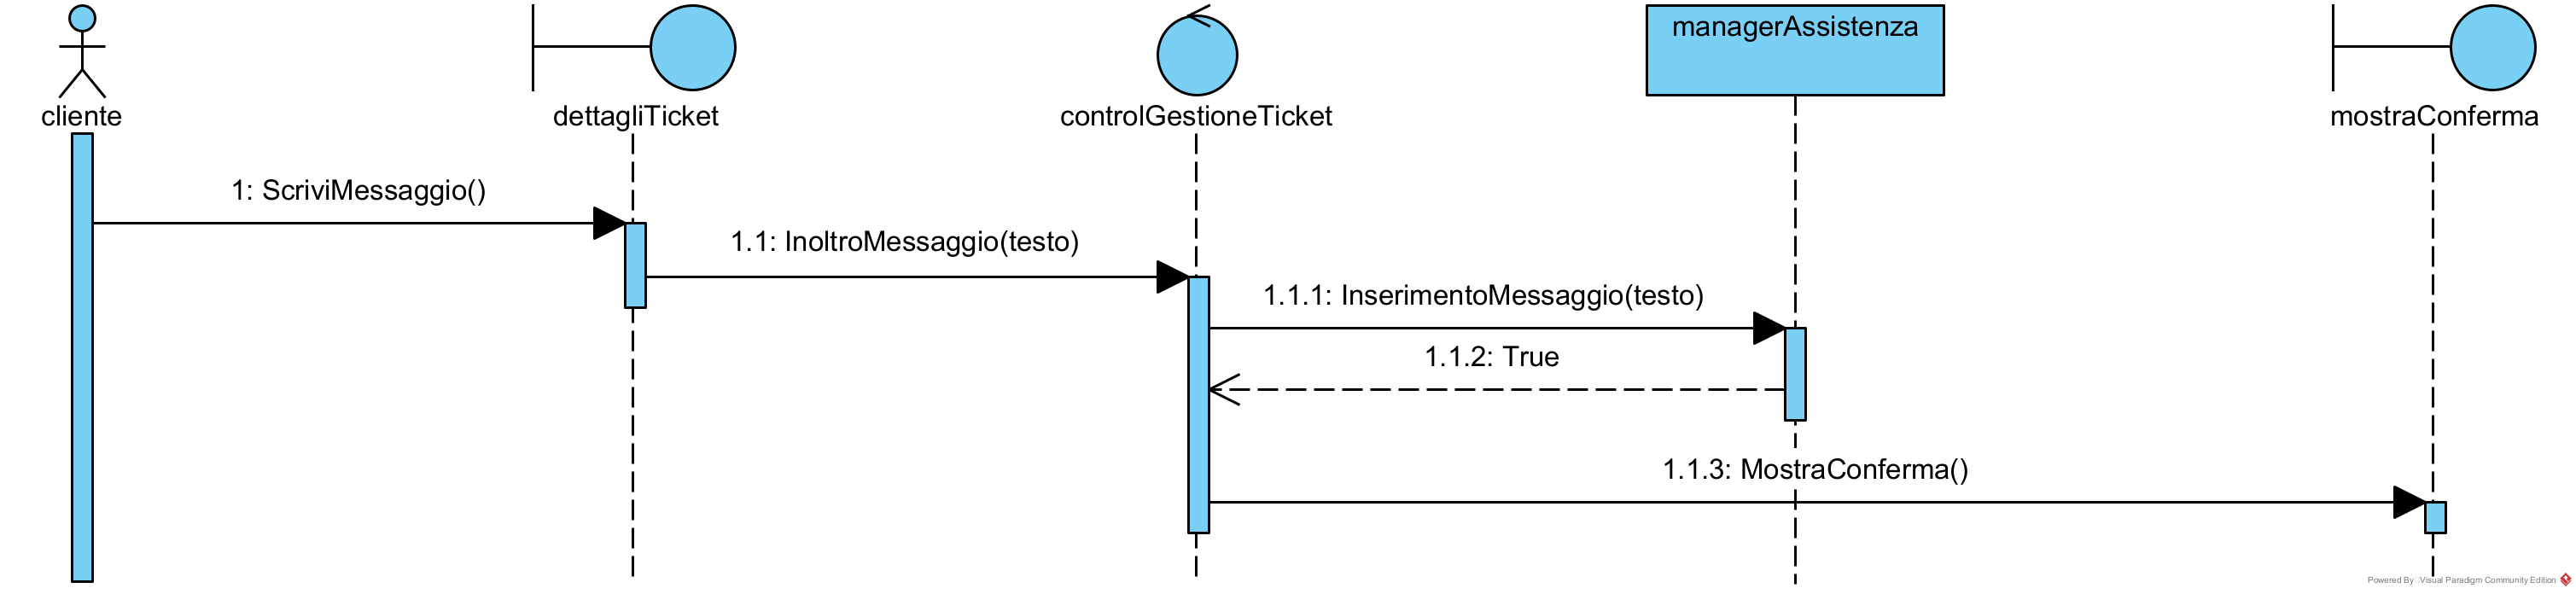
\includegraphics[width=\textwidth]{SequenceDiagram/ClienteTicketRisponde}
\end{center}

\begin{enumerate}
\item Dopo aver selezionato un ticket (\ref{SD:selezioneticketcliente}), l'utente usa il tasto ``Rispondi".
\item Gli viene quindi mostrato un modulo per inserire un nuovo messaggio in risposta al ticket.
\end{enumerate}

\subsubsection{Cliente chiude ticket}
\label{SD:chiusuraticket}

\begin{center}
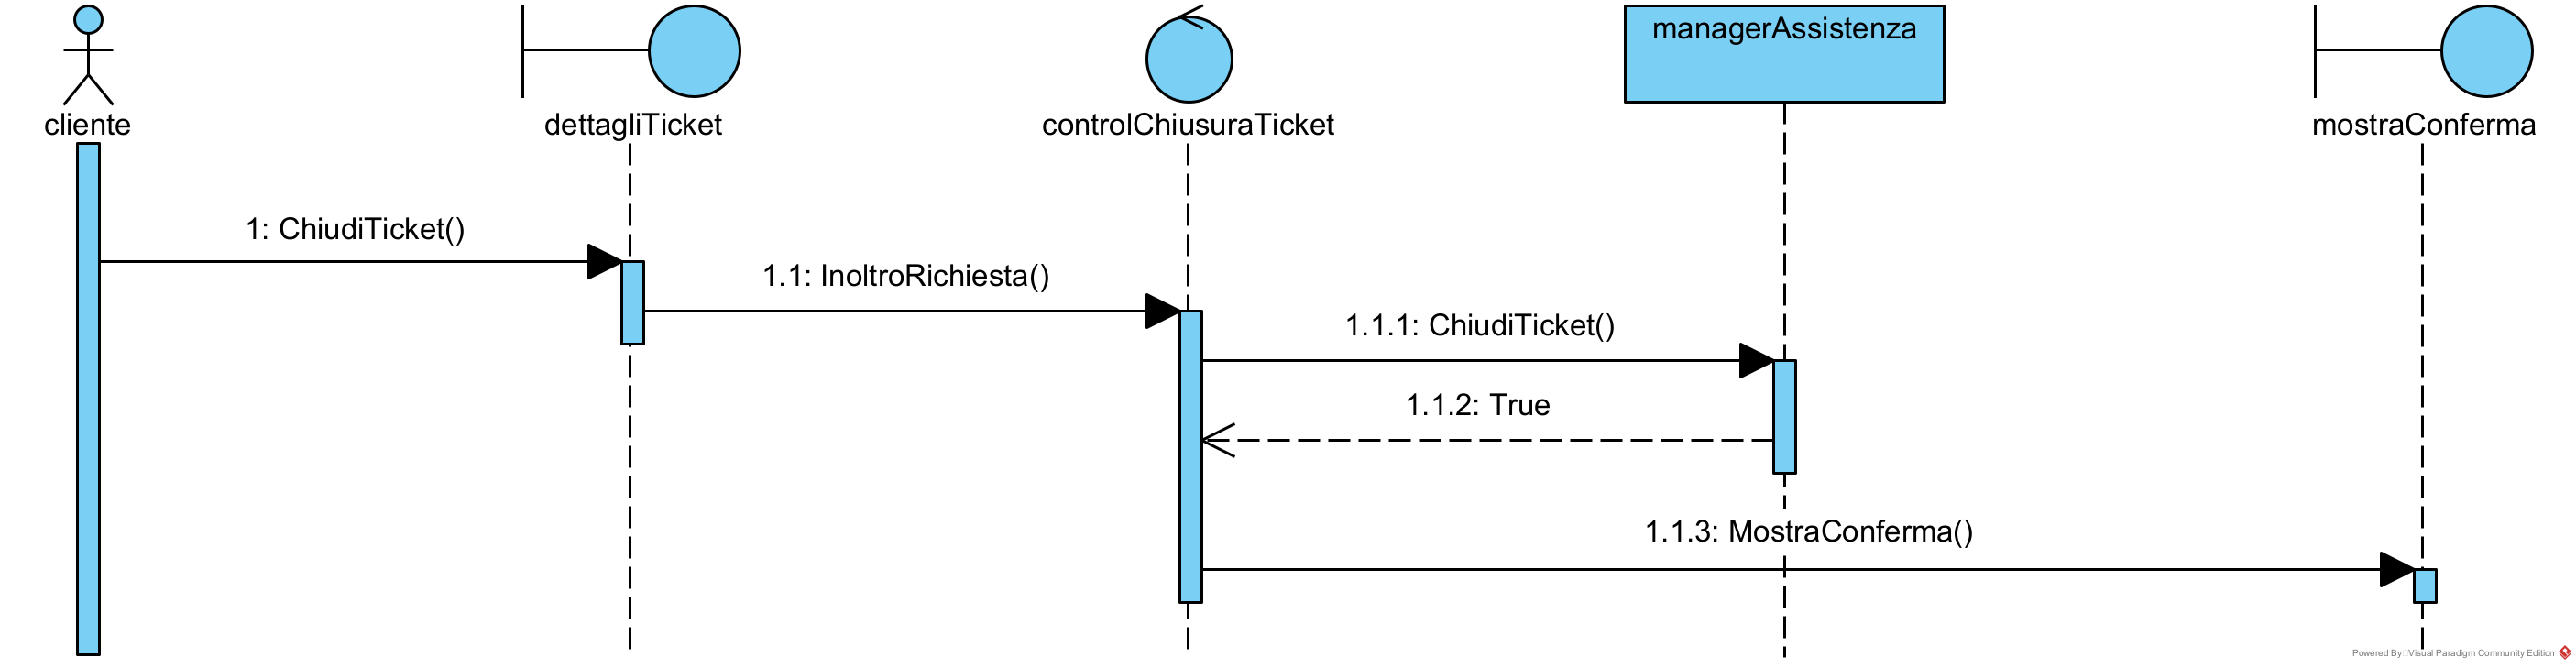
\includegraphics[width=\textwidth]{SequenceDiagram/ClienteTicketChiusura}
\end{center}

\begin{enumerate}
\item Dopo aver selezionato un ticket (\ref{SD:selezioneticketcliente}), l'utente usa il tasto ``Chiudi".
\item Il ticket viene dichiarato chiuso.
\item All'utente viene mostrata una pagina di conferma.
\end{enumerate}

\subsubsection{Cliente modifica password}
\label{SD:modificapw}

\begin{center}
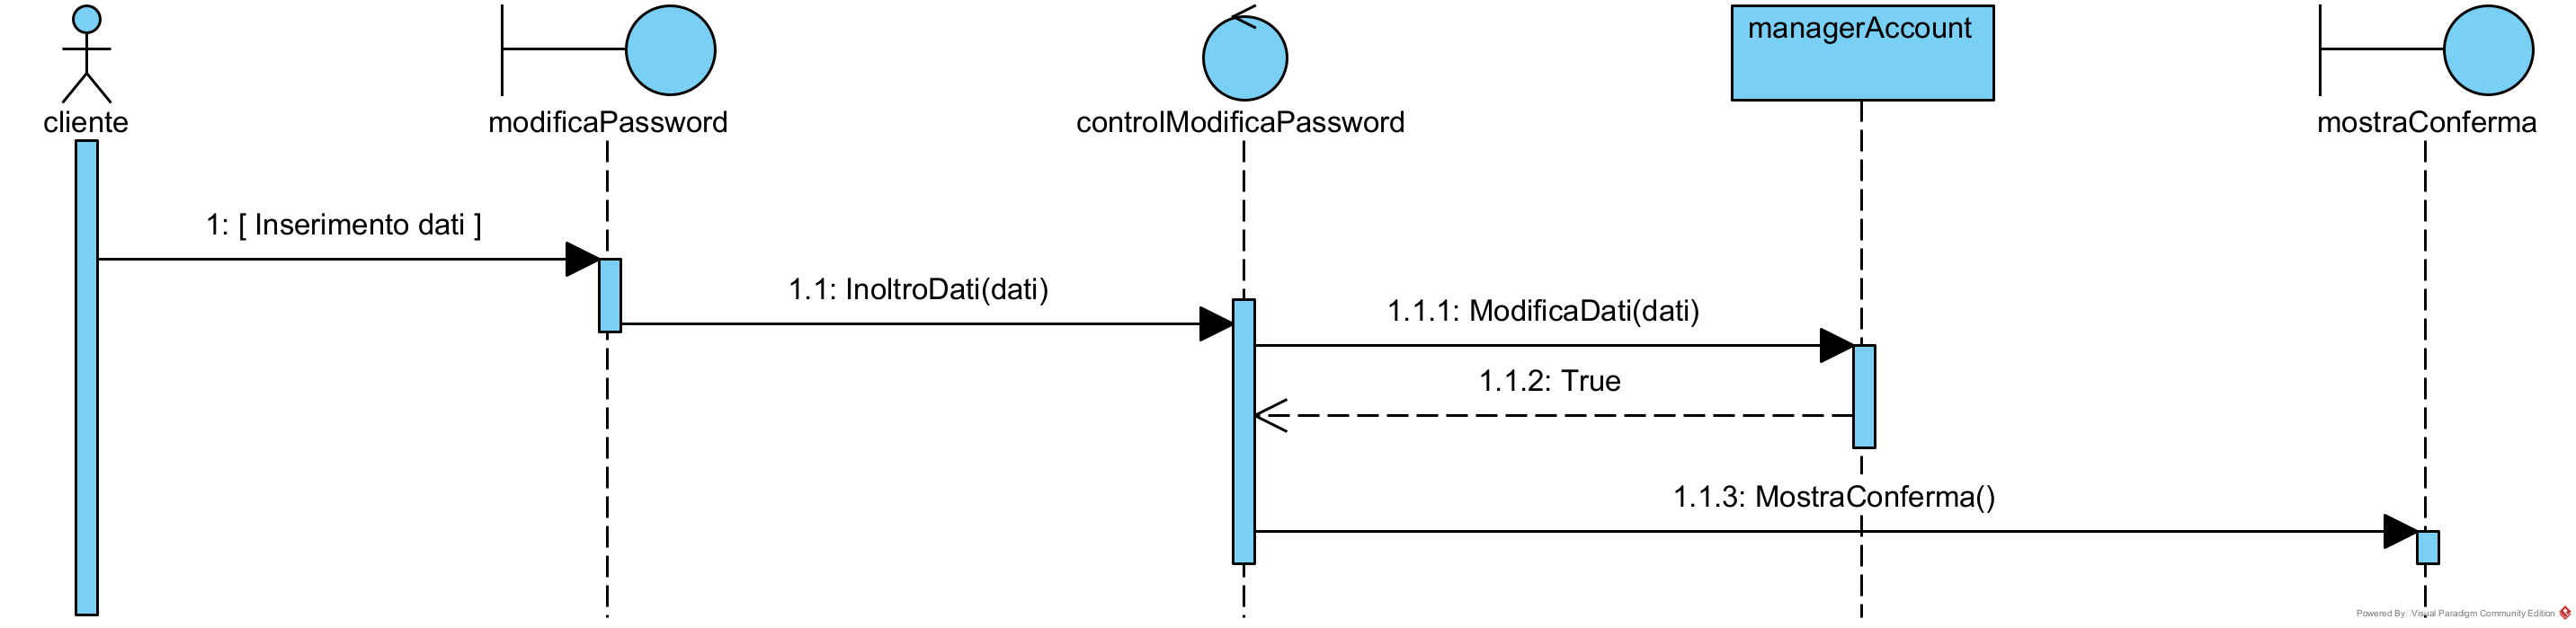
\includegraphics[width=\textwidth]{SequenceDiagram/ClientePasswordModifica}
\end{center}

\begin{enumerate}
\item Se un cliente ha dimenticato la password (\ref{SD:recuperopw}) o se un cliente vuole modificarla per altri motivi, viene rimandato a questo modulo per la modifica.
\item Il sistema provvede a criptare e memorizzare la nuova password per gli accessi futuri.
\end{enumerate}

\subsubsection{Cliente modifica profilo}
\label{SD:modificaprofilo}
\begin{center}
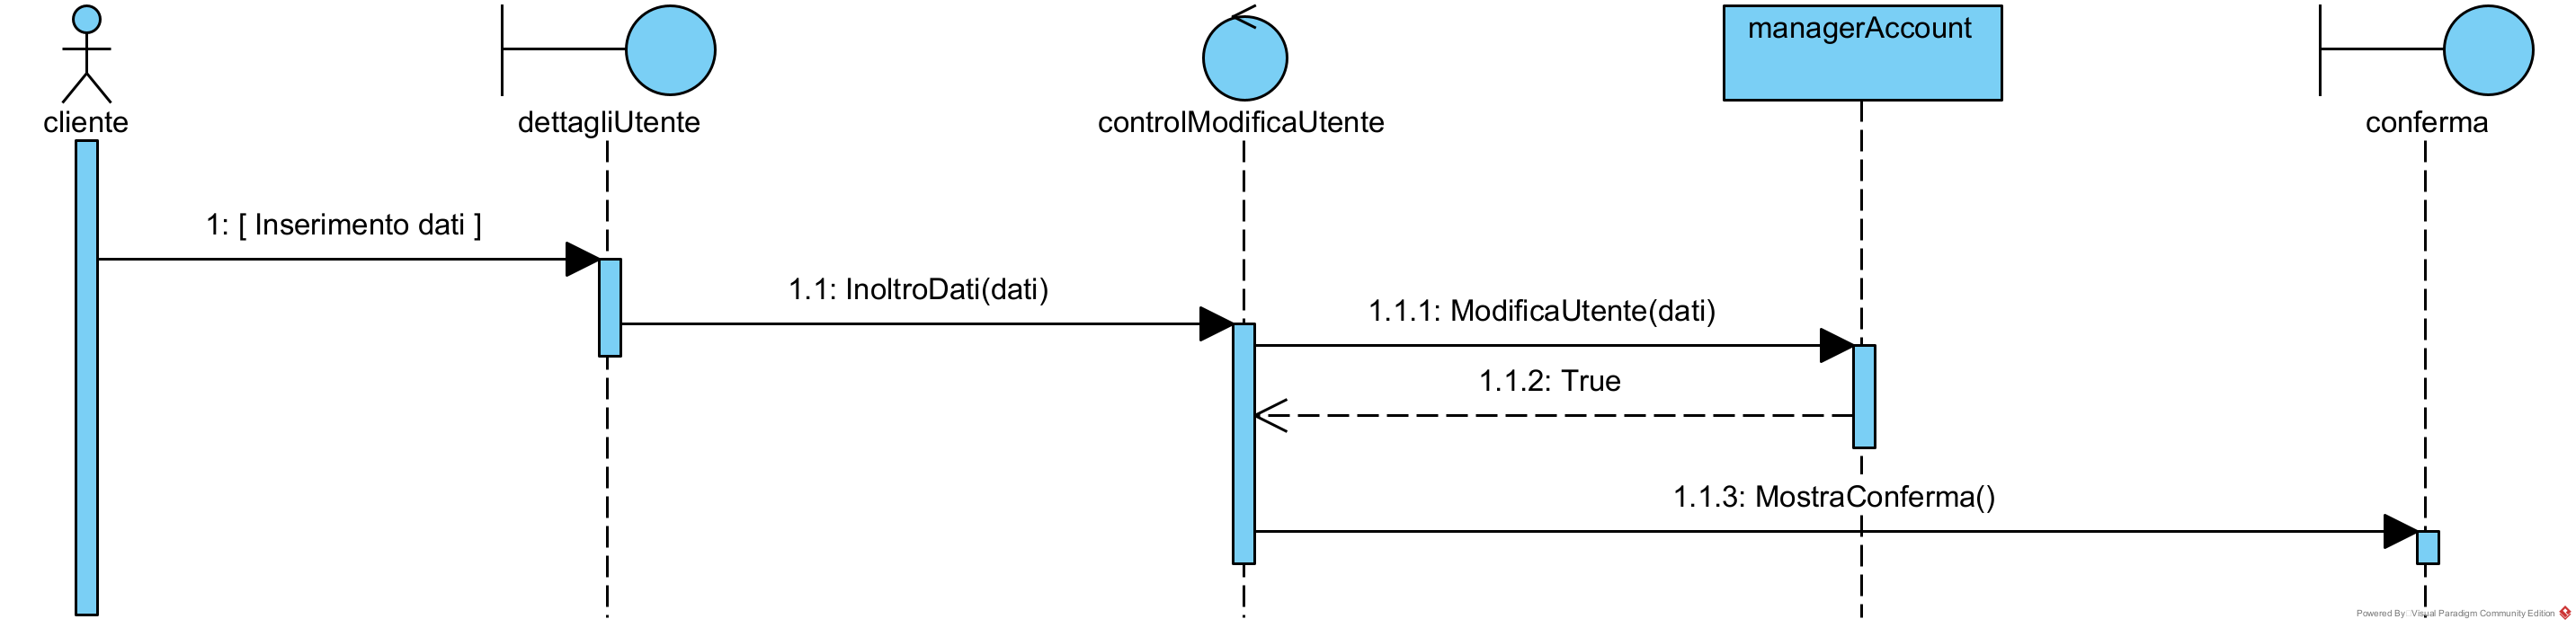
\includegraphics[width=\textwidth]{SequenceDiagram/ClienteProfiloModifica}
\end{center}

\begin{enumerate}
\item Se un cliente vuole modificare le informazioni del suo profilo come indirizzo, numero di carta di credito o altro, può farlo dalla pagina iniziale con il tasto dedicato.
\item Al cliente viene mostrato un modulo per la modifica dei dati, fatta eccezione per quelli cifrati come password e carta di credito, che possono essere soltanto sovrascritti.
\end{enumerate}

\newpage

\subsection{Centralinista}
\subsubsection{Centralinista elenca ticket}
\label{SD:centralinistaelencaticket}

\begin{center}
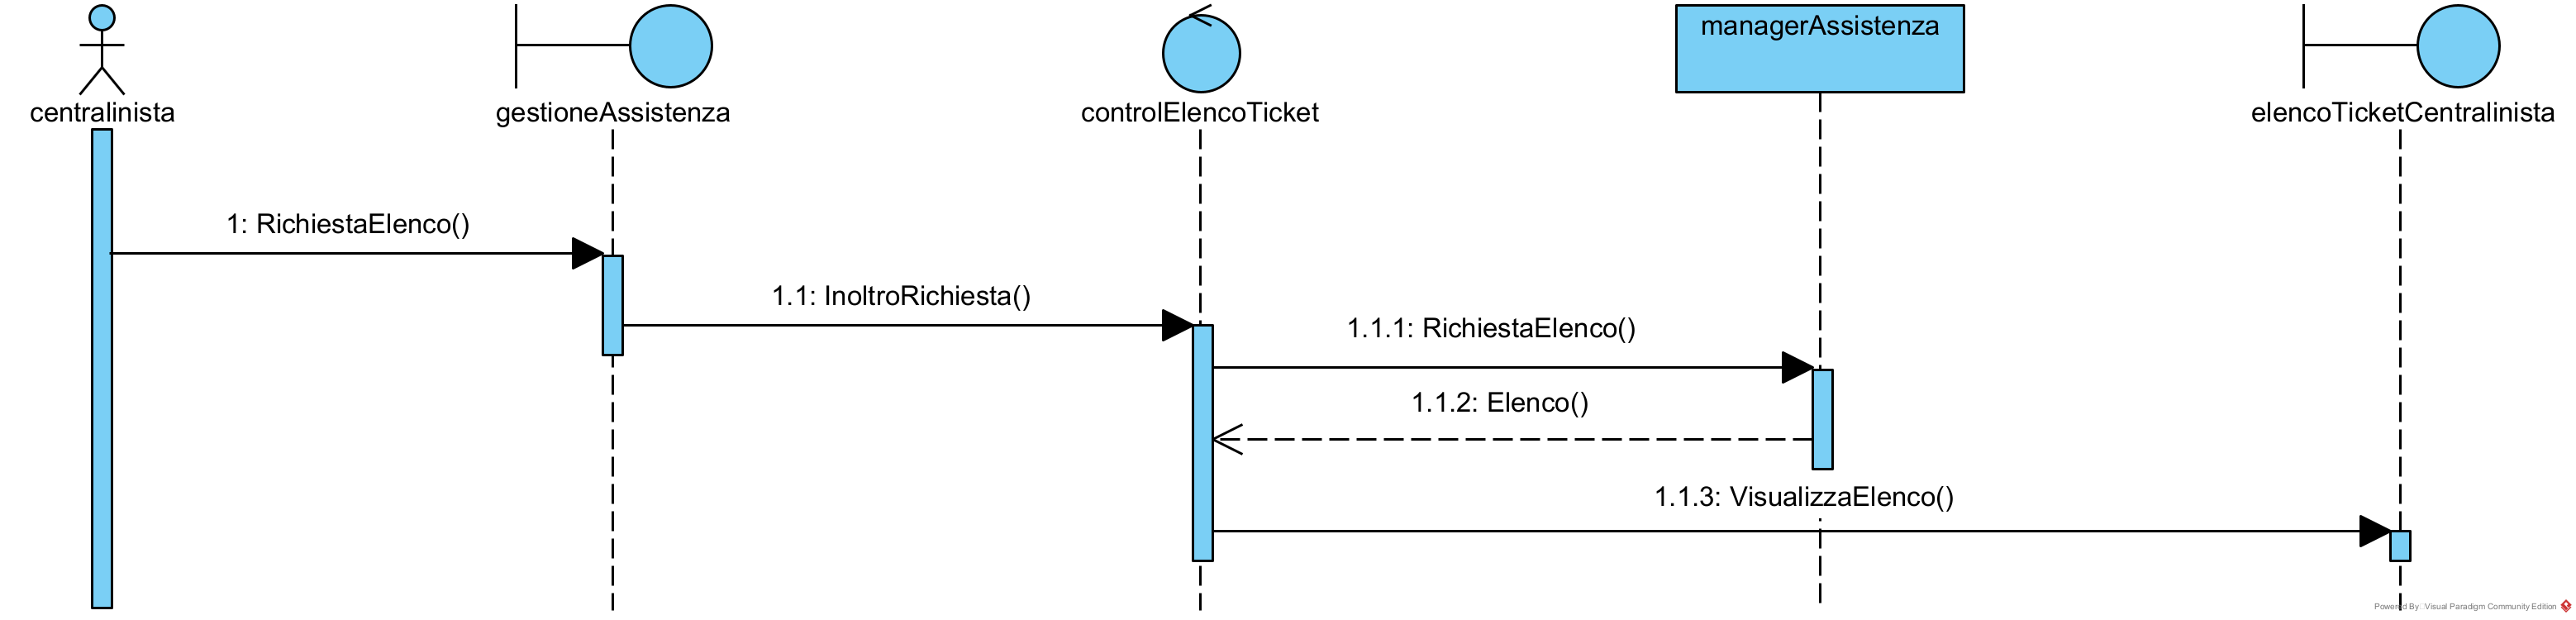
\includegraphics[width=\textwidth]{SequenceDiagram/CentralinistaTicketElenco}
\end{center}

\begin{enumerate}
\item Dopo essersi autenticato (\ref{SD:login}), il centralinista viene rimandato alla pagina iniziale dedicata ai centralinisti. 
\item Da lì può scegliere di visualizzare l'elenco dei ticket in attesa di risposta, ordinati per data crescente.
\end{enumerate}

\subsubsection{Centralinista seleziona un ticket}
\label{SD:selezioneticketcentralinista}

\begin{center}
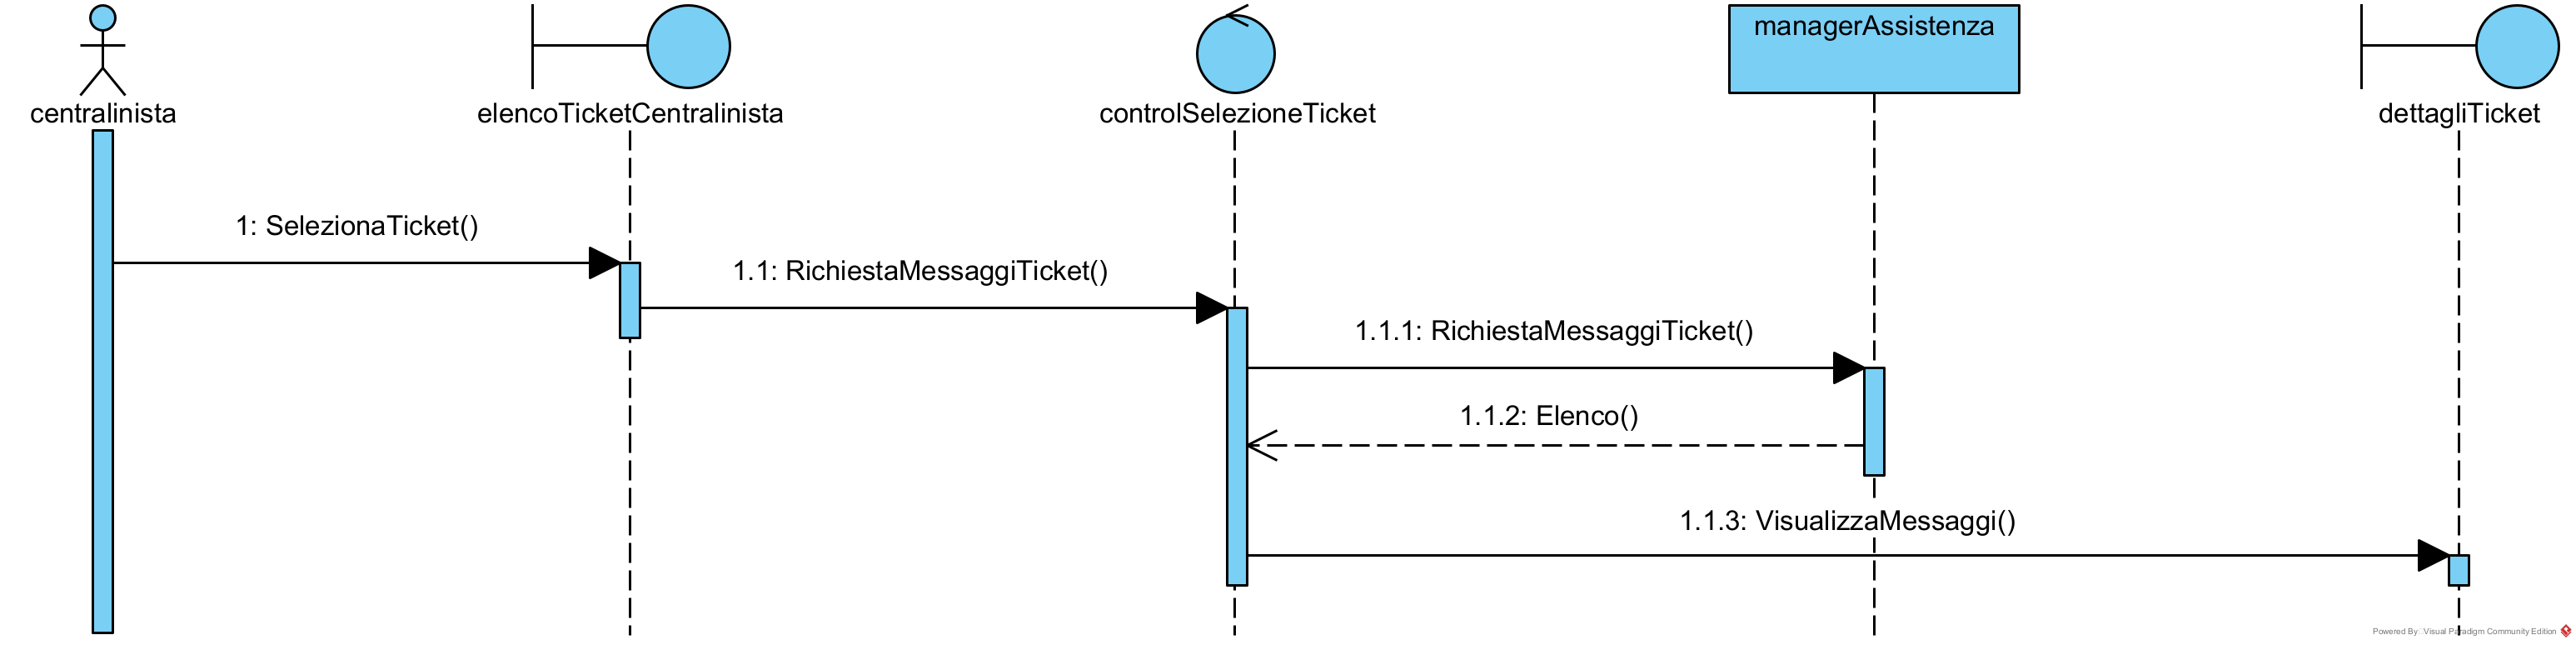
\includegraphics[width=\textwidth]{SequenceDiagram/CentralinistaTicketSeleziona}
\end{center}

\begin{enumerate}
\item Dall'elenco dei ticket (\ref{SD:centralinistaelencaticket}), il centralinista fa click su uno dei ticket attualmente aperti che nello stato di attesa.
\item Lo stato di quel ticket viene cambiato a "In elaborazione".
\item Vengono mostrati tutti i messaggi inviati fino a quel momento.
\end{enumerate}

\newpage

\subsubsection{Centralinista risponde ad un ticket}
\label{SD:rispostaticketcentralinista}

\begin{center}
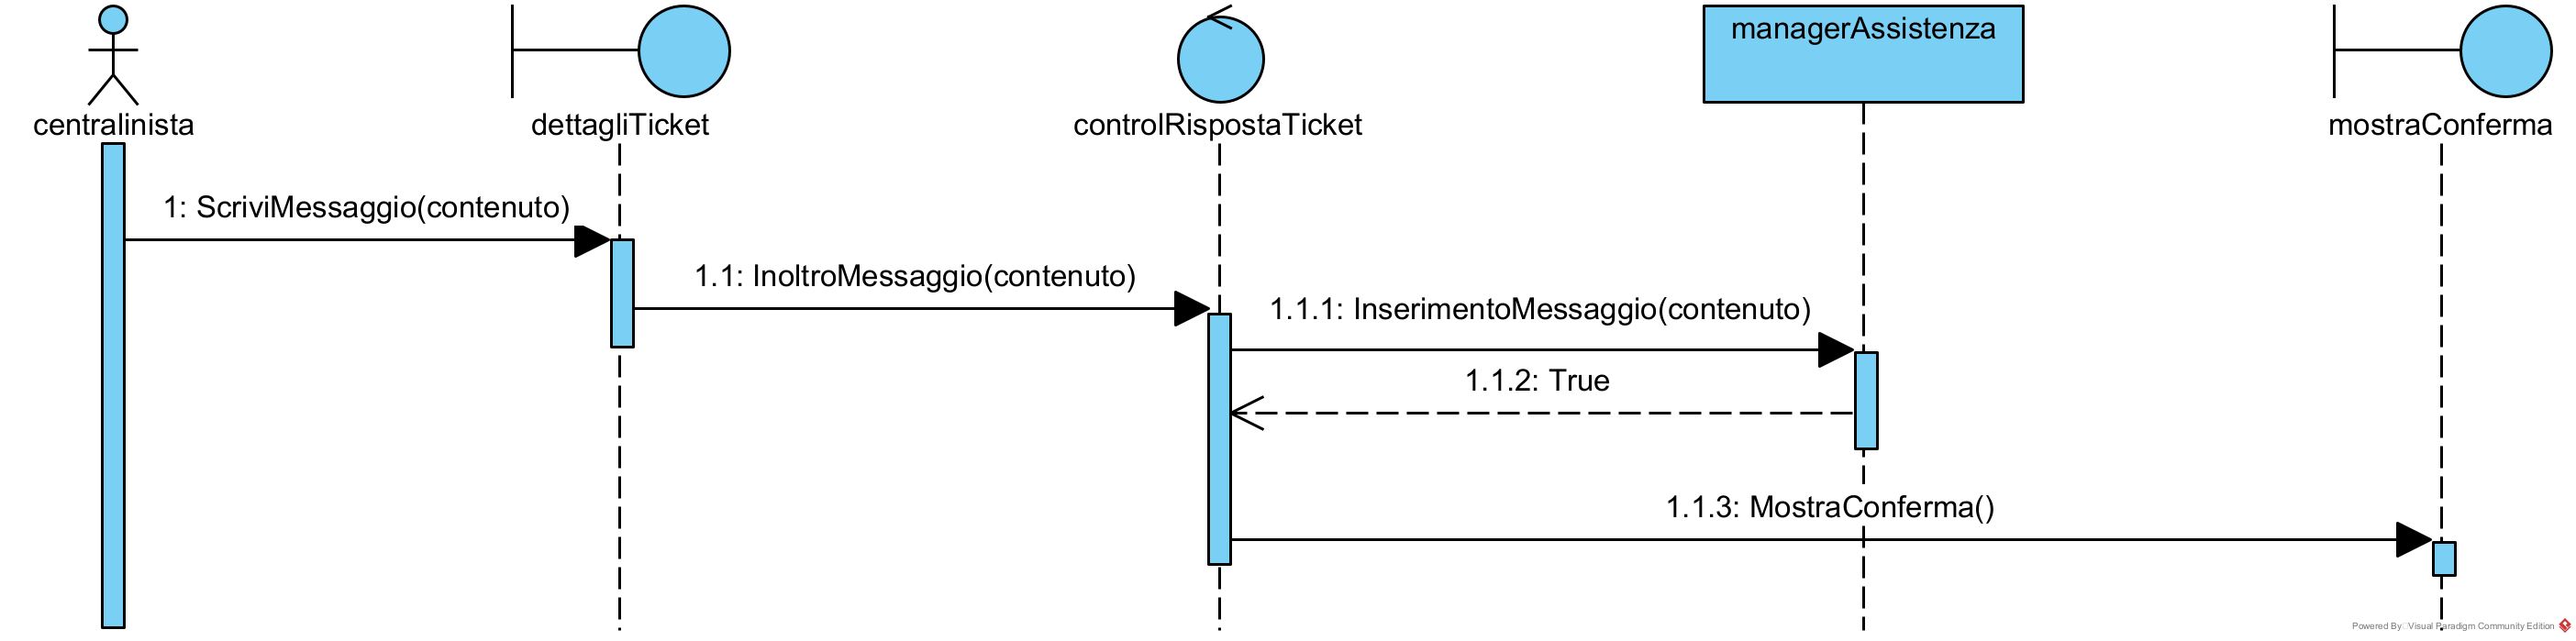
\includegraphics[width=\textwidth]{SequenceDiagram/CentralinistaTicketRisponde}
\end{center}

\begin{enumerate}
\item Dopo aver selezionato un ticket (\ref{SD:selezioneticketcentralinista}), il centralinista usa il tasto ``Rispondi".
\item Gli viene quindi mostrato un modulo per inserire un nuovo messaggio in risposta al ticket.
\item Dopo aver inviato il messaggio, lo stato passa da "In elaborazione" a "In attesa del cliente".
\end{enumerate}

\subsubsection{Centralinista visualizza elenco vendite}
\label{SD:elencovenditecentralinista}

\begin{center}
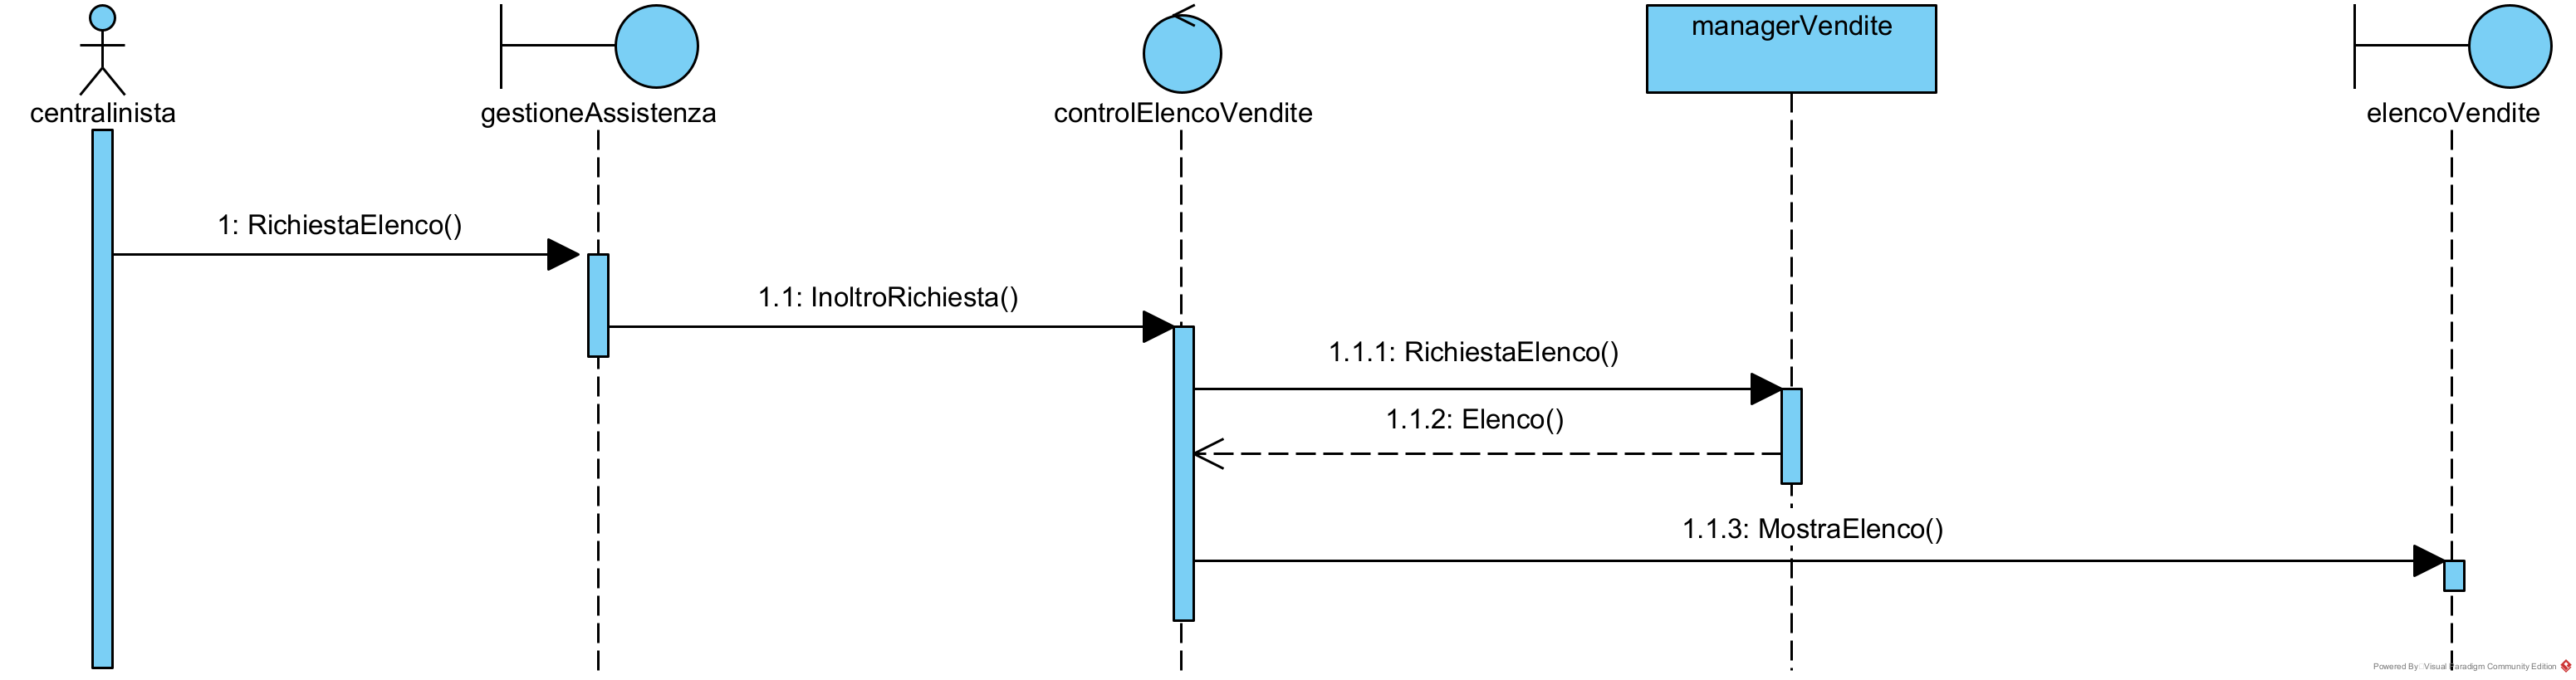
\includegraphics[width=\textwidth]{SequenceDiagram/CentralinistaVenditeElenco}
\end{center}

\begin{enumerate}
\item Dopo essersi autenticato (\ref{SD:login}), il centralinista viene rimandato alla sua homepage. 
\item Da lì potrà scegliere di visualizzare l'elenco delle vendite in attesa di risposta, ordinate per data crescente.
\end{enumerate}

\newpage

\subsubsection{Centralinista seleziona una vendita}
\label{SD:selezionevenditacentralinista}

\begin{center}
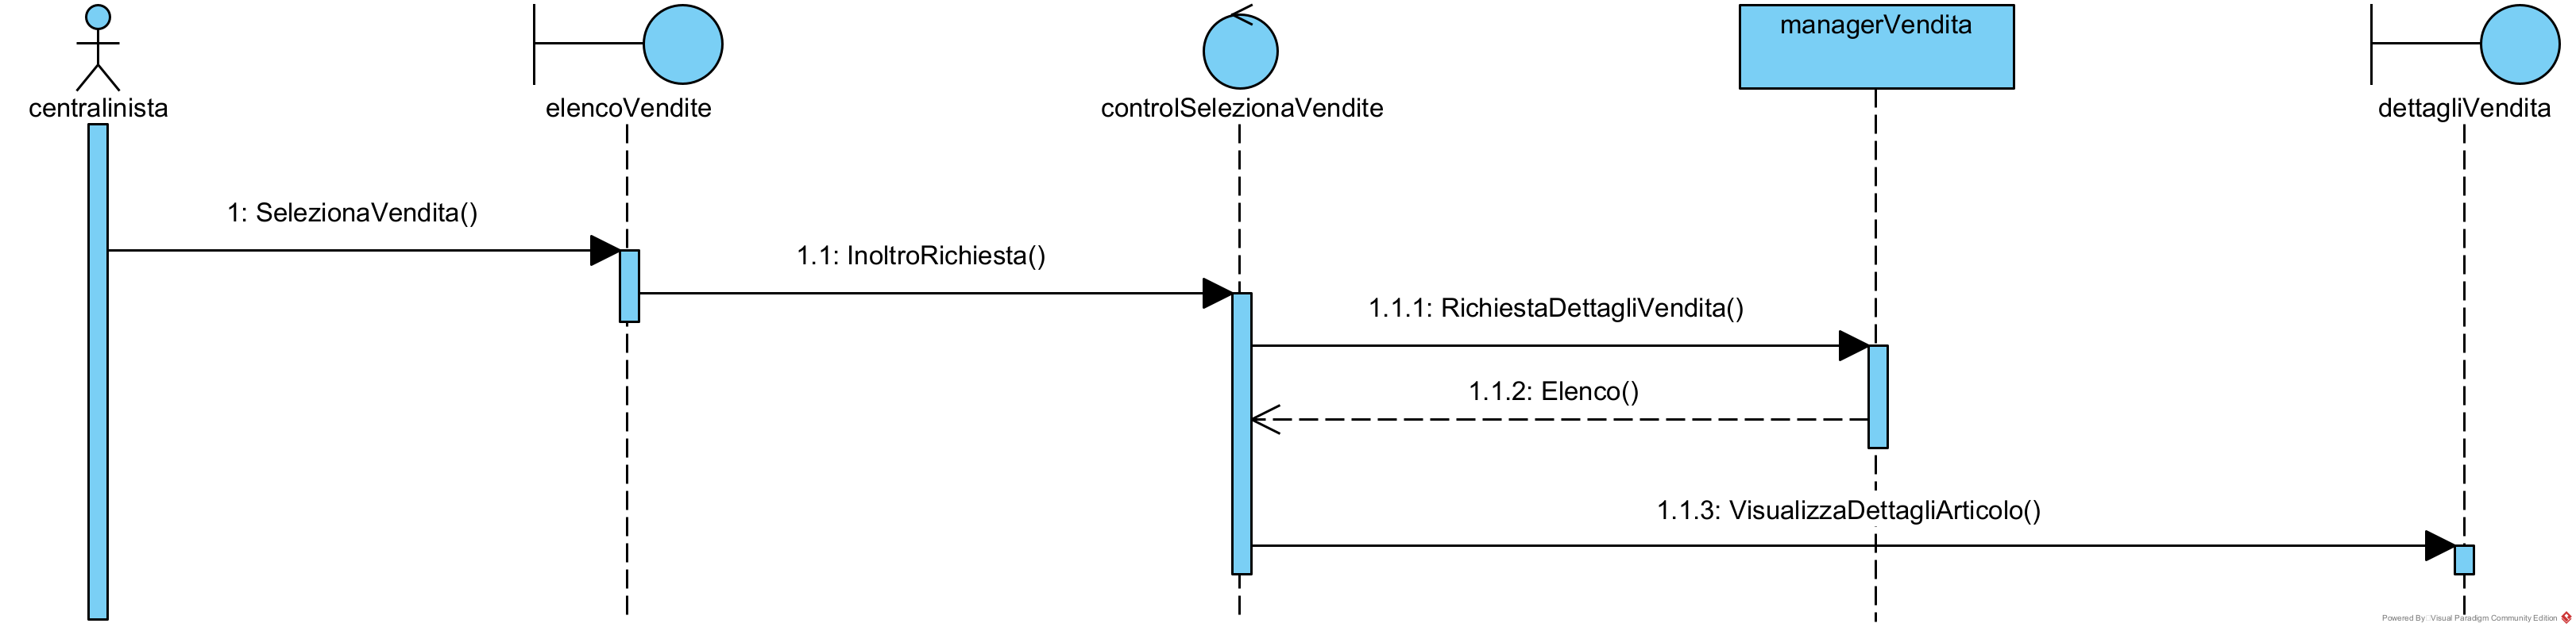
\includegraphics[width=\textwidth]{SequenceDiagram/CentralinistaVenditaSeleziona}
\end{center}

\begin{enumerate}
\item Dall'elenco dei ticket (\ref{SD:centralinistaelencaticket}), il centralinista fa click su una delle vendite attualmente in attesa di conferma.
\item Lo stato della vendita passa a "In elaborazione".
\item Vengono visualizzati tutti i dettagli di quella vendita.
\end{enumerate}

\subsubsection{Centralinista autorizza una vendita}
\label{SD:centralinistaautorizza}
\begin{center}
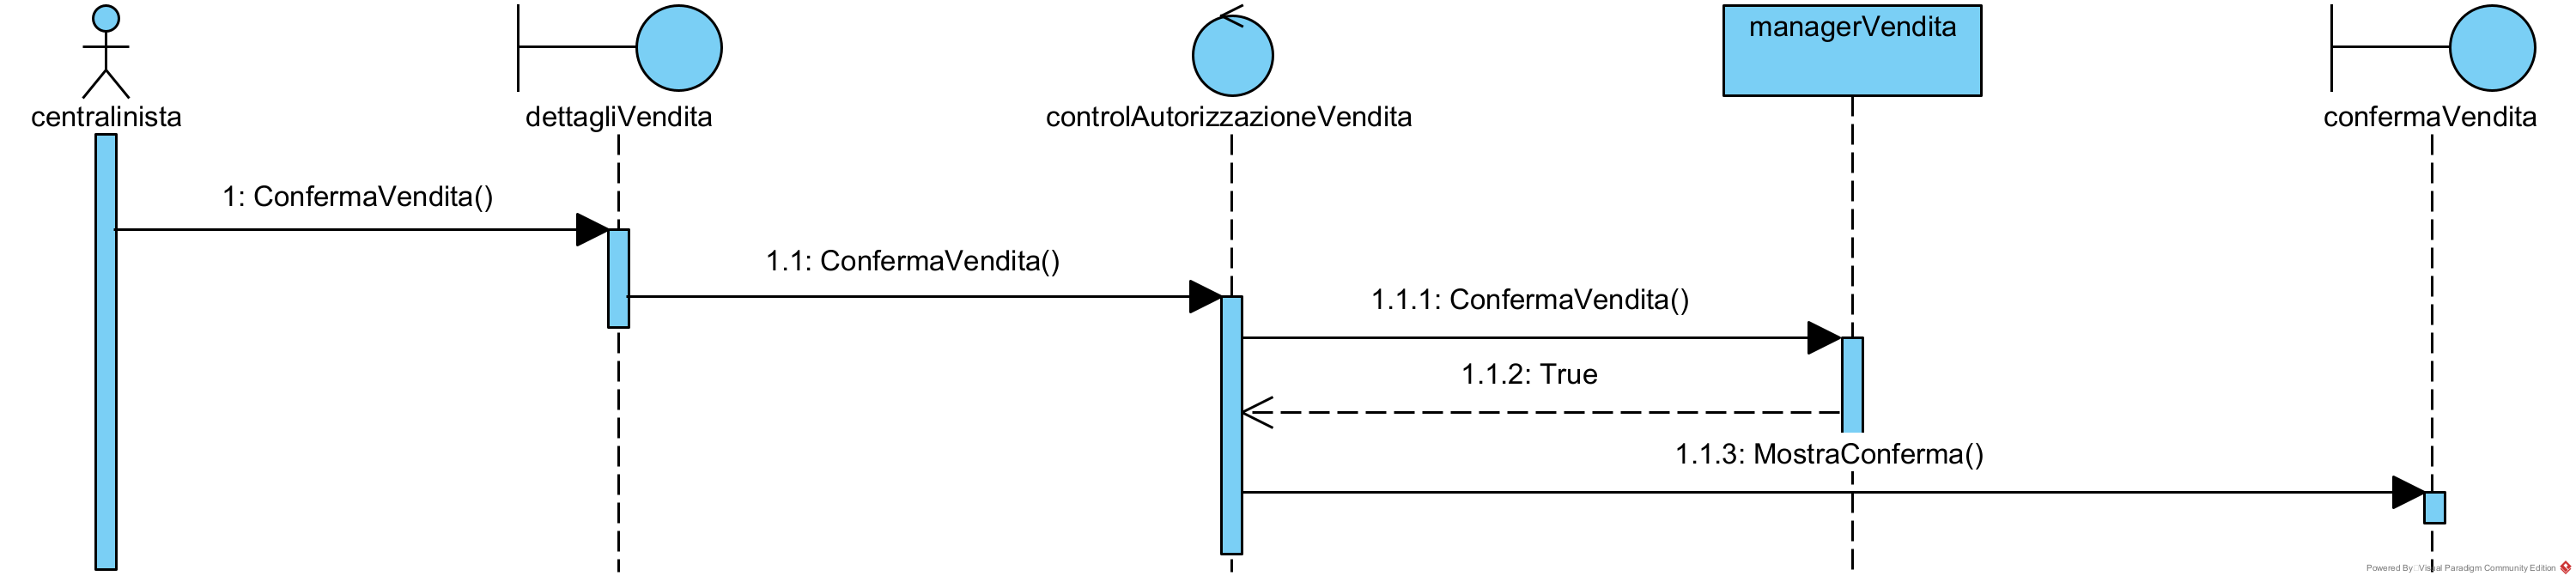
\includegraphics[width=\textwidth]{SequenceDiagram/CentralinistaVenditaAutorizza}
\end{center}

\begin{enumerate}
\item Dopo aver selezionato una vendita (\ref{SD:selezionevenditacentralinista}), il centralinista può autorizzare o rifiutare una vendita.
\end{enumerate}

\newpage

\subsection{Magazziniere}
\subsubsection{Magazziniere elenca ordini}
\label{SD:magazzinierevisualizzaelenco}
\begin{center}
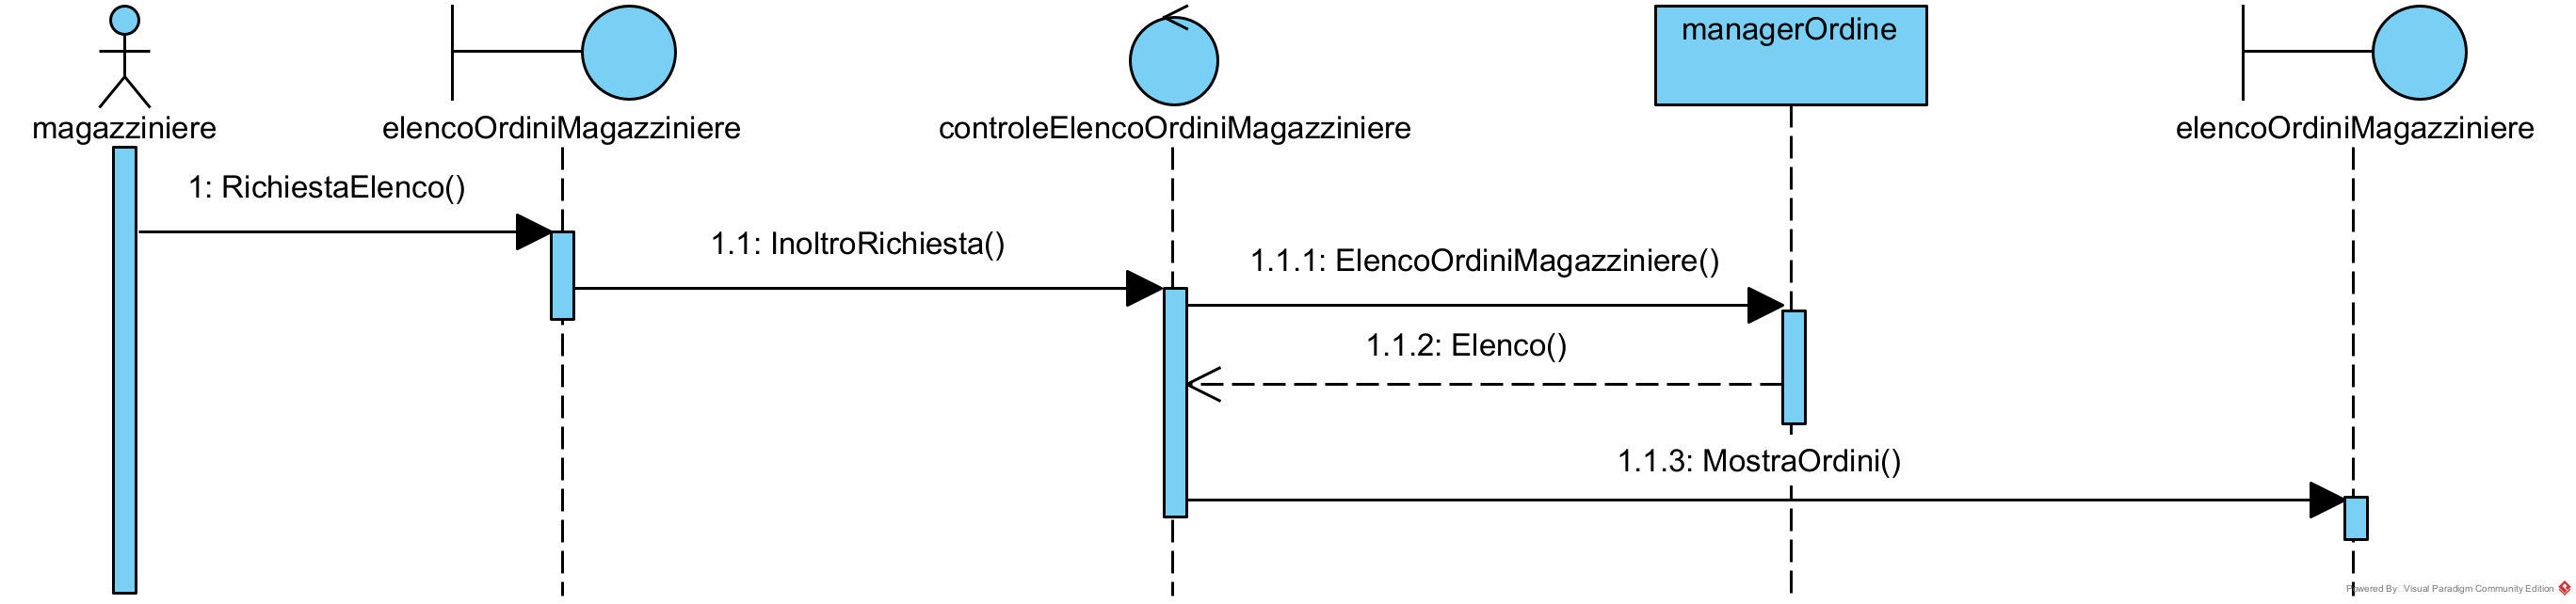
\includegraphics[width=\textwidth]{SequenceDiagram/MagazziniereOrdiniElenco}
\end{center}

\begin{enumerate}
\item Dopo essersi autenticato (\ref{SD:login}), il magazziniere può usare il tasto ``Ordini" per essere rimandato all'elenco degli ordini in attesa di spedizione.
\end{enumerate}

\subsubsection{Magazziniere elabora ordine}
\label{SD:magazziniereblocca}
\begin{center}
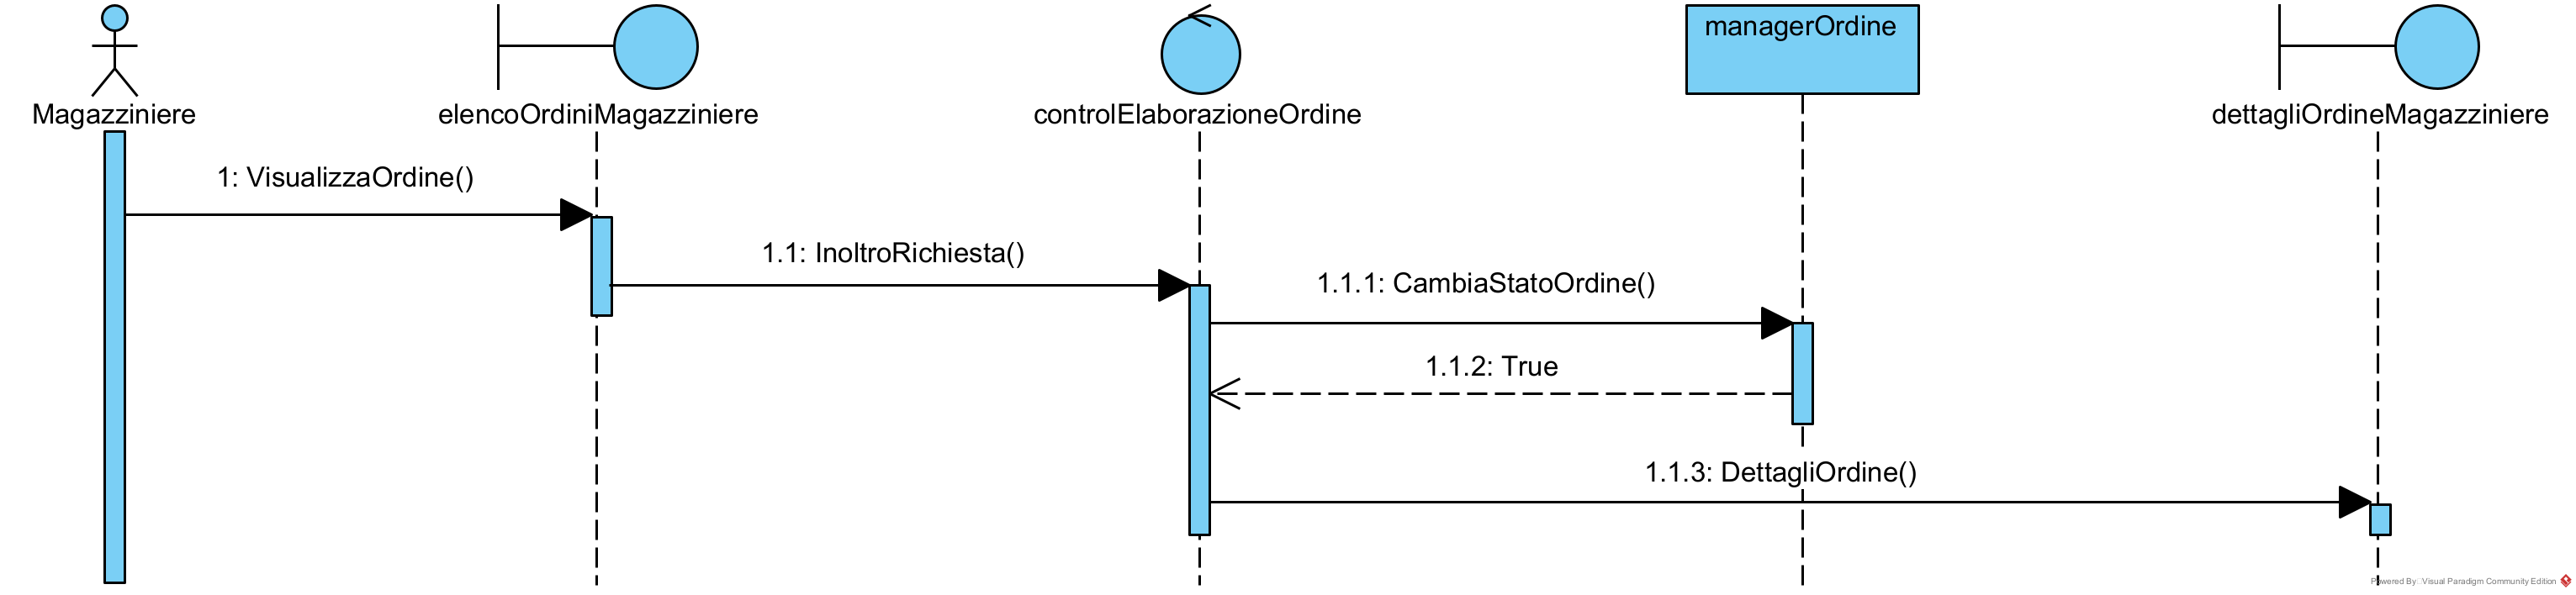
\includegraphics[width=\textwidth]{SequenceDiagram/MagazziniereOrdineVisualizza}
\end{center}

\begin{enumerate}
\item Dall'elenco degli ordini (\ref{SD:magazzinierevisualizzaelenco}), il magazziniere può visualizzare i dettagli di un ordine. Nel fare ciò cambia lo stato dell'ordine a ``In elaborazione", in modo che non appaia ad altri magazzinieri.
\end{enumerate}

\subsubsection{Magazziniere spedisce ordine}
\label{SD:magazzinierespedisce}
\begin{center}
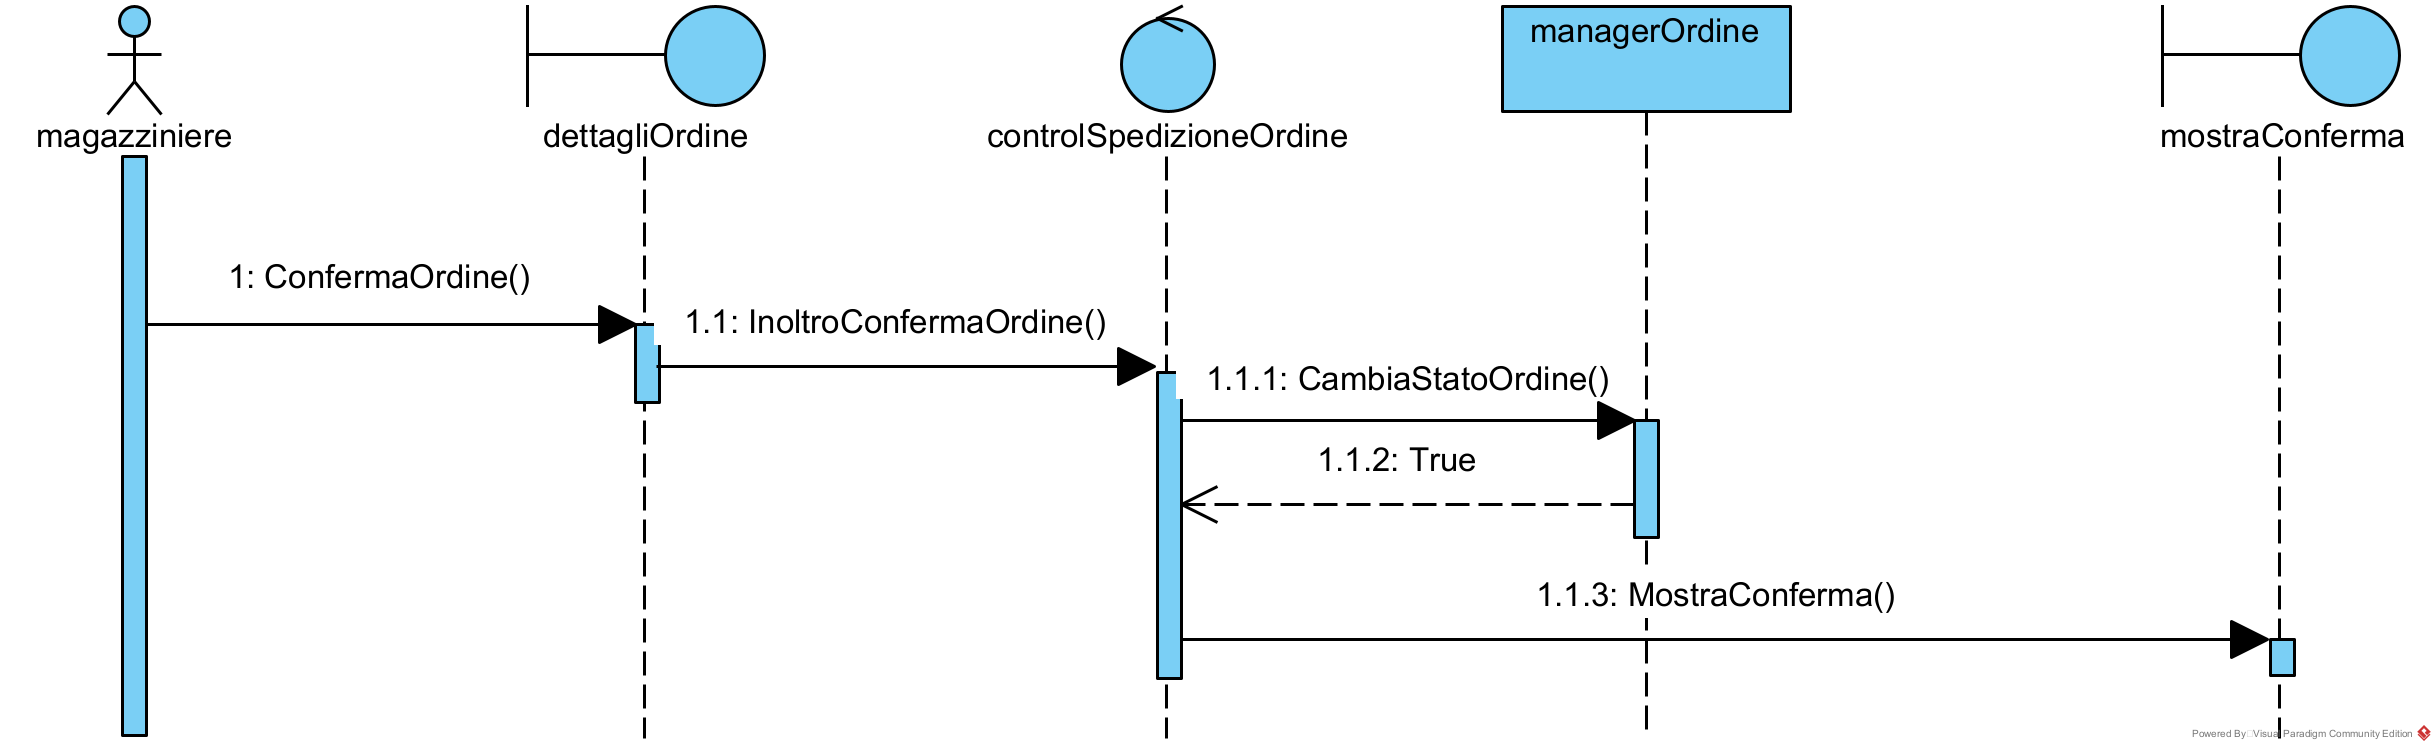
\includegraphics[width=\textwidth]{SequenceDiagram/MagazziniereOrdineSpedisce}
\end{center}

\begin{enumerate}
\item Dai dettagli di un ordine (\ref{SD:magazziniereblocca}), il magazziniere può accettare (\checkmark) un ordine.
\end{enumerate}

\subsubsection{Magazziniere annulla ordine}
\label{SD:magazziniereannulla}
\begin{center}
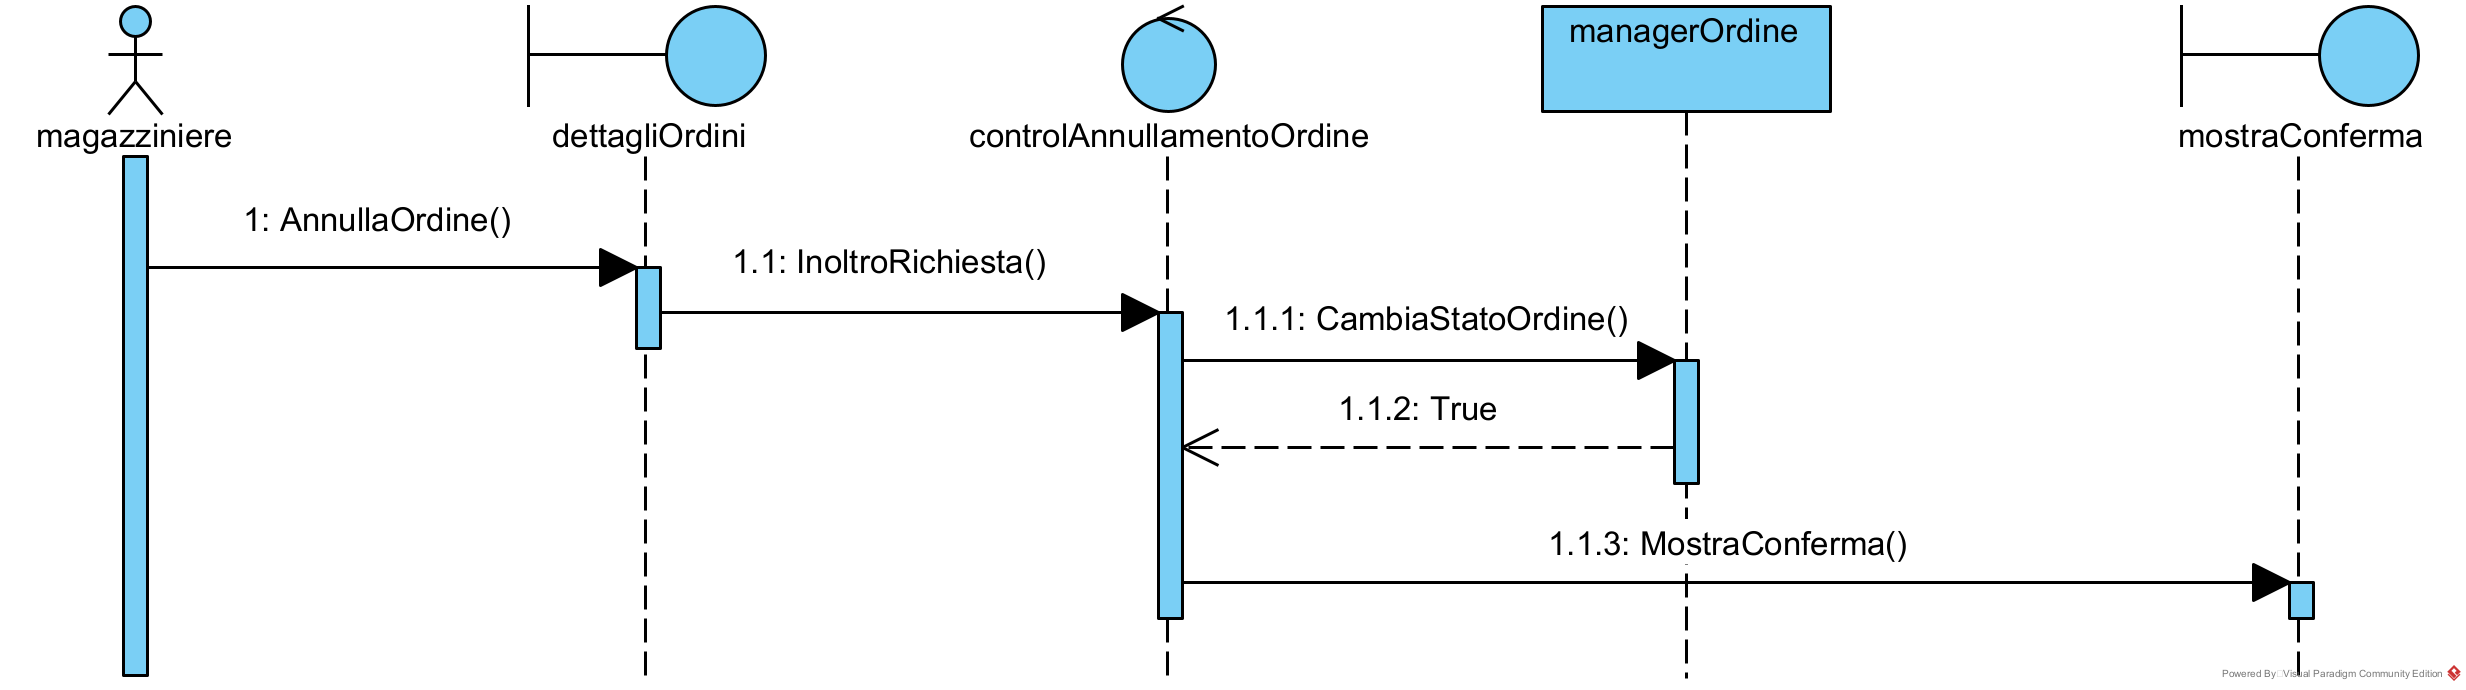
\includegraphics[width=\textwidth]{SequenceDiagram/MagazziniereOrdineAnnulla}
\end{center}

\begin{enumerate}
\item Dopo essersi autenticato (\ref{SD:login}), il magazziniere può usare il tasto ``Rimborsi" per essere rimandato all'elenco dei rimborsi in attesa di conferma.
\end{enumerate}

\subsubsection{Magazziniere elenca rimborsi}
\label{SD:magazziniereelencorimborsi}
\begin{center}
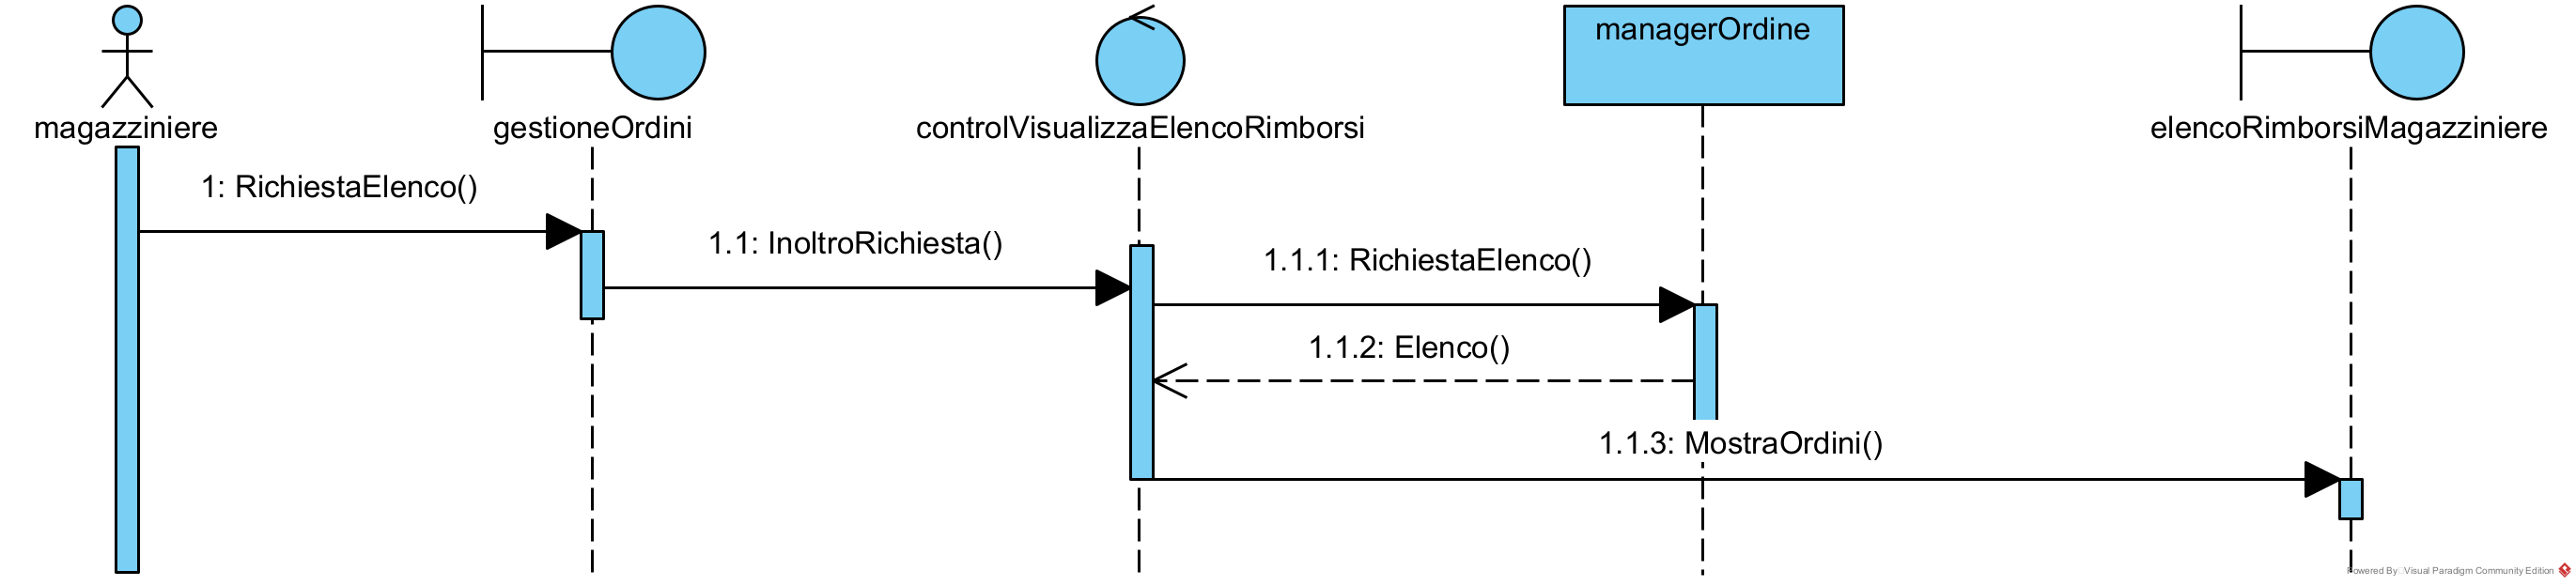
\includegraphics[width=\textwidth]{SequenceDiagram/MagazziniereRimborsoElenco}
\end{center}

\begin{enumerate}
\item Dopo essersi autenticato (\ref{SD:login}), il magazziniere può usare il tasto ``Rimborsi" per essere rimandato all'elenco dei rimborsi in attesa di conferma.
\end{enumerate}

\subsubsection{Magazziniere accetta rimborso}
\label{SD:magazzrimborsook}
\begin{center}
\includegraphics[width=\textwidth]{SequenceDiagram/magazziniereRimborsoAccetta}
\end{center}

\begin{enumerate}
\item Dai dettagli di un ordine (\ref{SD:magazziniereblocca}), il magazziniere può confermare la ricezione di un ordine e cambiare lo stato di un ordine a ``Rimborsato".
\end{enumerate}

\newpage

\subsection{Amministratore catalogo}
\subsubsection{Amministratore catalogo ricerca articolo}
\label{SD:amcatvisualizzaelenco}
\begin{center}
\includegraphics[width=\textwidth]{SequenceDiagram/AmministratoreCatalogoVenditaRicerca}
\end{center}

\begin{enumerate}
\item L'amministratore del catalogo può effettuare una ricerca tra gli articoli messi in vendita dalla piattaforma.
\end{enumerate}

\subsubsection{Amministratore catalogo seleziona articolo}
\label{SD:amcatselezionaarticolo}
\begin{center}
\includegraphics[width=\textwidth]{SequenceDiagram/AmministratoreCatalogoVenditaSeleziona}
\end{center}

\begin{enumerate}
\item Dai risultati della ricerca (\ref{SD:amcatvisualizzaelenco}), l'amministratore del catalogo può selezionare uno degli articoli per visualizzarne i dettagli.
\item Viene rimandato a una pagina con i dettagli dell'articolo.
\end{enumerate}

\subsubsection{Amministratore catalogo inserisce articolo}
\label{SD:amcatinseriscearticolo}
\begin{center}
\includegraphics[width=\textwidth]{SequenceDiagram/AmministratoreCatalogoVenditaCrea}
\end{center}

\begin{enumerate}
\item Dall'elenco (\ref{SD:amcatvisualizzaelenco}), l'amministratore del catalogo può inserire un nuovo articolo usando il tasto ``Nuovo articolo".
\item Viene rimandato ad un modulo per l'inserimento dei dati necessari come nome, prezzo, quantità disponibile e foto.
\item L'articolo viene immediatamente messo in vendita.
\end{enumerate}

\subsubsection{Amministratore catalogo modifica articolo}
\label{SD:amcatmodificaarticolo}
\begin{center}
\includegraphics[width=\textwidth]{SequenceDiagram/AmministratoreCatalogoVenditaModifica}
\end{center}

\begin{enumerate}
\item Dai risultati della ricerca (\ref{SD:amcatvisualizzaelenco}), l'amministratore del catalogo può modificare i dettagli di un articolo.
\item Cliccando il tasto ``Modifica" visualizzerà una pagina con un modulo per la modifica delle informazioni.
\end{enumerate}

\subsubsection{Amministratore catalogo rimuove articolo}
\label{SD:amcatrimuovearticolo}
\begin{center}
\includegraphics[width=\textwidth]{SequenceDiagram/AmministratoreCatalogoVenditaRimuove}
\end{center}

\begin{enumerate}
\item Dai risultati della ricerca (\ref{SD:amcatvisualizzaelenco}), l'amministratore del catalogo può rimuovere un articolo usando il tasto ``Rimuovi".
\end{enumerate}

\newpage

\subsection{Amministratore personale}
\subsubsection{Amministratore personale ricerca dipendente}
\label{SD:amperricerca}
\begin{center}
\includegraphics[width=\textwidth]{SequenceDiagram/AmministratorePersonaleDipendenteRicerca}
\end{center}

\begin{enumerate}
\item L'amministratore del personale può effettuare una ricerca tra i dipendenti.
\end{enumerate}

\subsubsection{Amministratore personale seleziona dipendente}
\label{SD:amperselezione}
\begin{center}
\includegraphics[width=\textwidth]{SequenceDiagram/AmministratorePersonaleDipendenteSeleziona}
\end{center}

\begin{enumerate}
\item Dall'elenco (\ref{SD:amcatvisualizzaelenco}), l'amministratore del personale potrà selezionare uno dei dipendenti per visualizzarne i dettagli e le statistiche come il numero di ordini spediti o il numero di ticket a cui hanno risposto, in base alla tipologia di dipendente.
\end{enumerate}

\subsubsection{Amministratore personale inserisce dipendente}
\label{SD:amperinserisce}
\begin{center}
\includegraphics[width=\textwidth]{SequenceDiagram/AmministratorePersonaleDipendenteInserisce}
\end{center}

\begin{enumerate}
\item Dall'elenco (\ref{SD:amcatvisualizzaelenco}), l'amministratore del personale può inserire un nuovo dipendente.
\item Viene rimandato ad un modulo per l'inserimento dei dati richiesti come nome, cognome, indirizzo e ruolo.
\end{enumerate}

\subsubsection{Amministratore personale modifica dipendente}
\label{SD:ampermodifica}
\begin{center}
\includegraphics[width=\textwidth]{SequenceDiagram/AmministratorePersonaleDipendenteModifica}
\end{center}

\begin{enumerate}
\item Dalla pagina dei dettagli di un dipendente (\ref{SD:amperselezione}), l'amministratore del personale può modificare i dettagli di un dipendente usando il tasto ``Modifica".
\item Visualizza una pagina con un modulo per la modifica delle informazioni.
\end{enumerate}

\subsubsection{Amministratore personale rimuove dipendente}
\label{SD:amperrimuove}
\begin{center}
\includegraphics[width=\textwidth]{SequenceDiagram/AmministratorePersonaleDipendenteRimuove}
\end{center}


\begin{enumerate}
\item Dalla pagina dei dettagli di un articolo (\ref{SD:amcatselezionaarticolo}), l'amministratore del catalogo può rimuovere un articolo usando il tasto ``Rimuovi".
\item Visualizza una pagina di conferma.
\end{enumerate}

\newpage

\section{Statechart Diagram}

\subsection{Ordine}
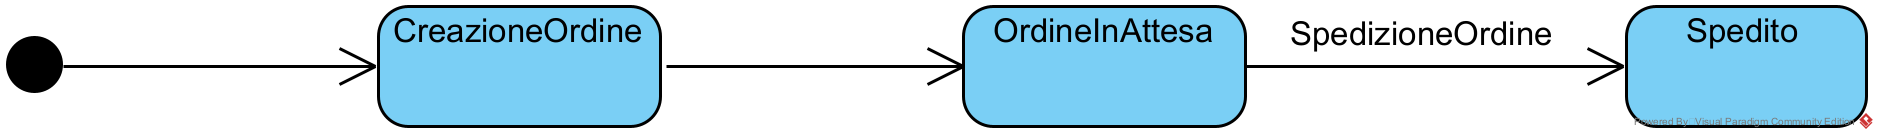
\includegraphics[width=\textwidth]{StateChart/Ordine}

\subsection{Ticket}
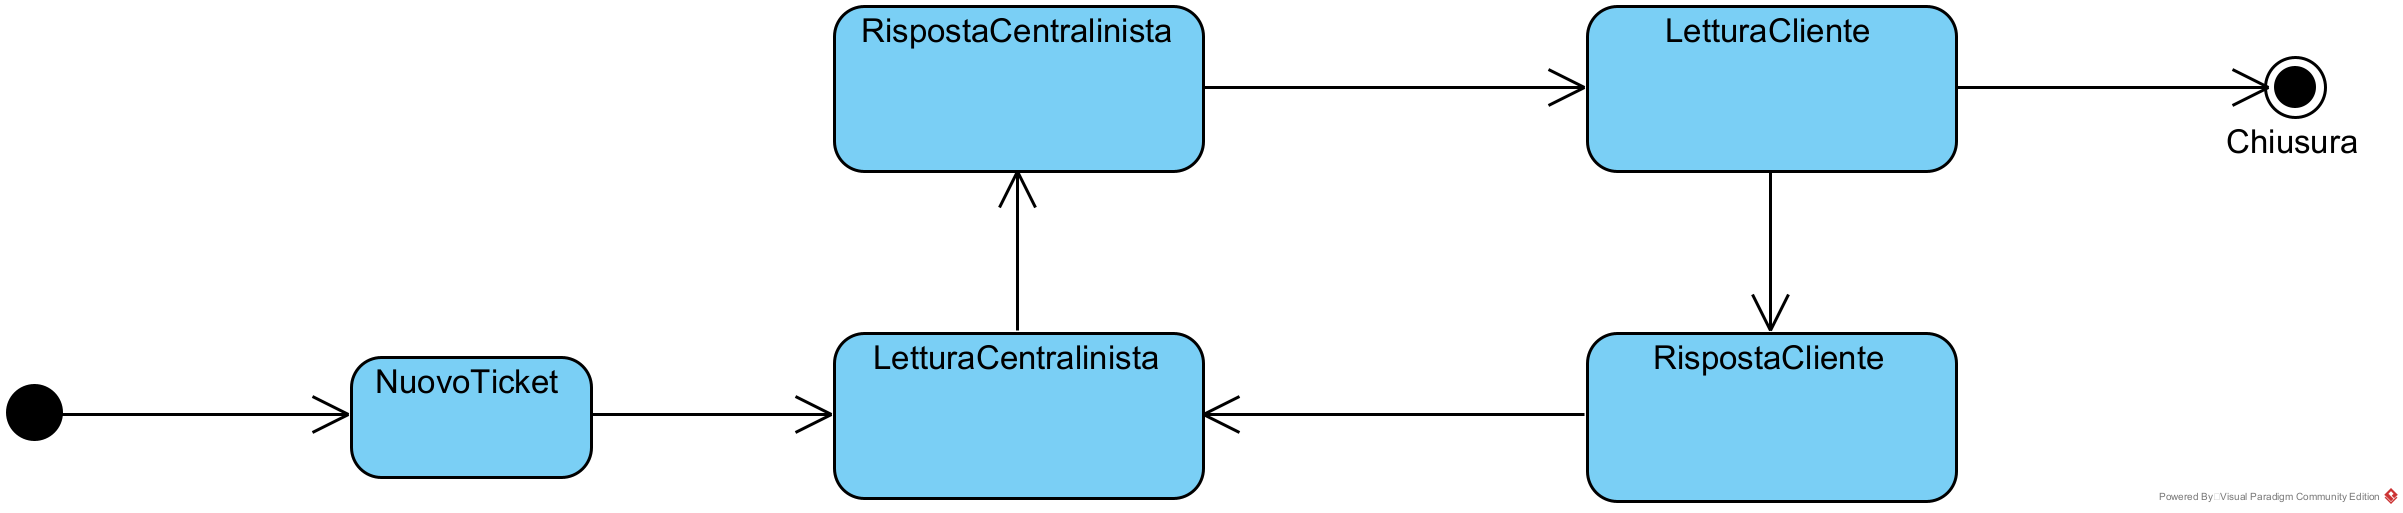
\includegraphics[width=\textwidth]{StateChart/Ticket}

\subsection{Vendita}
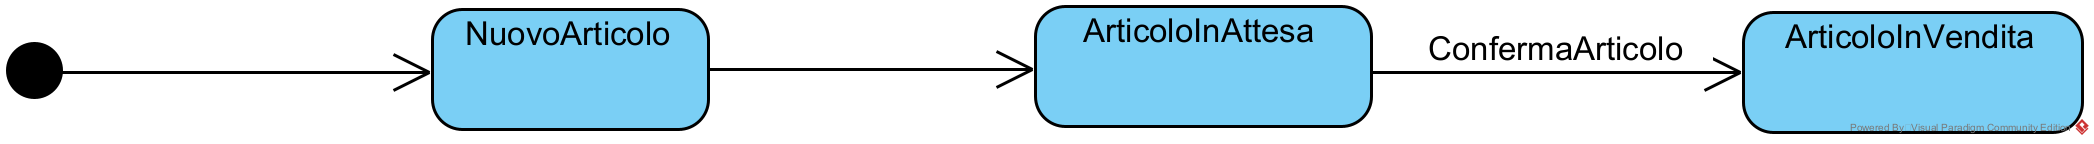
\includegraphics[width=\textwidth]{StateChart/Vendita}

\newpage

\section{Activity Diagram}

\subsection{Registrazione}
\begin{center}
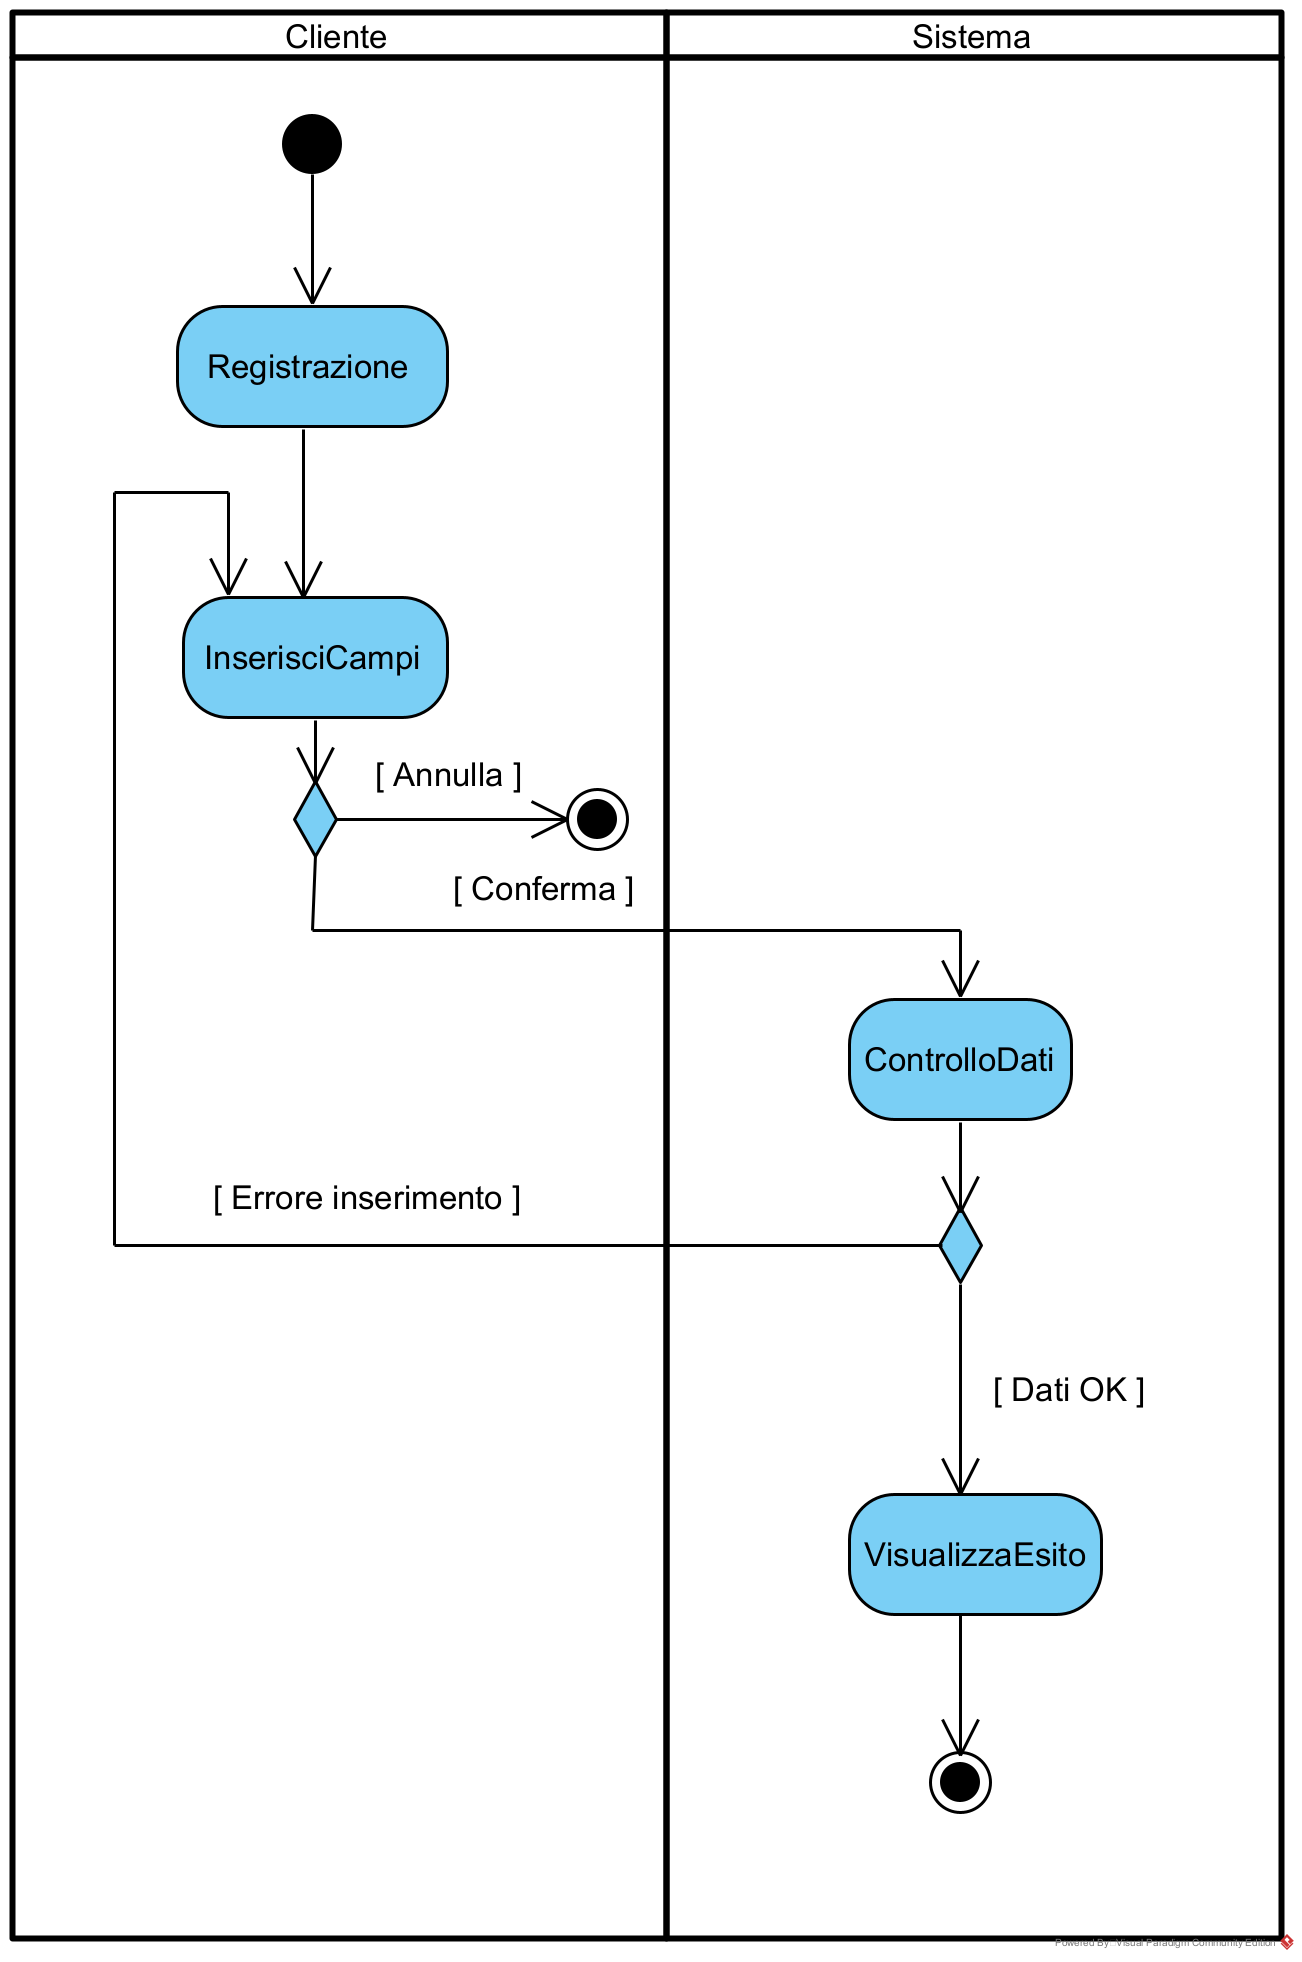
\includegraphics[width=\textwidth]{ActivityDiagram/ClienteRegistrazione}
\end{center}

\subsection{Acquisto}
\begin{center}
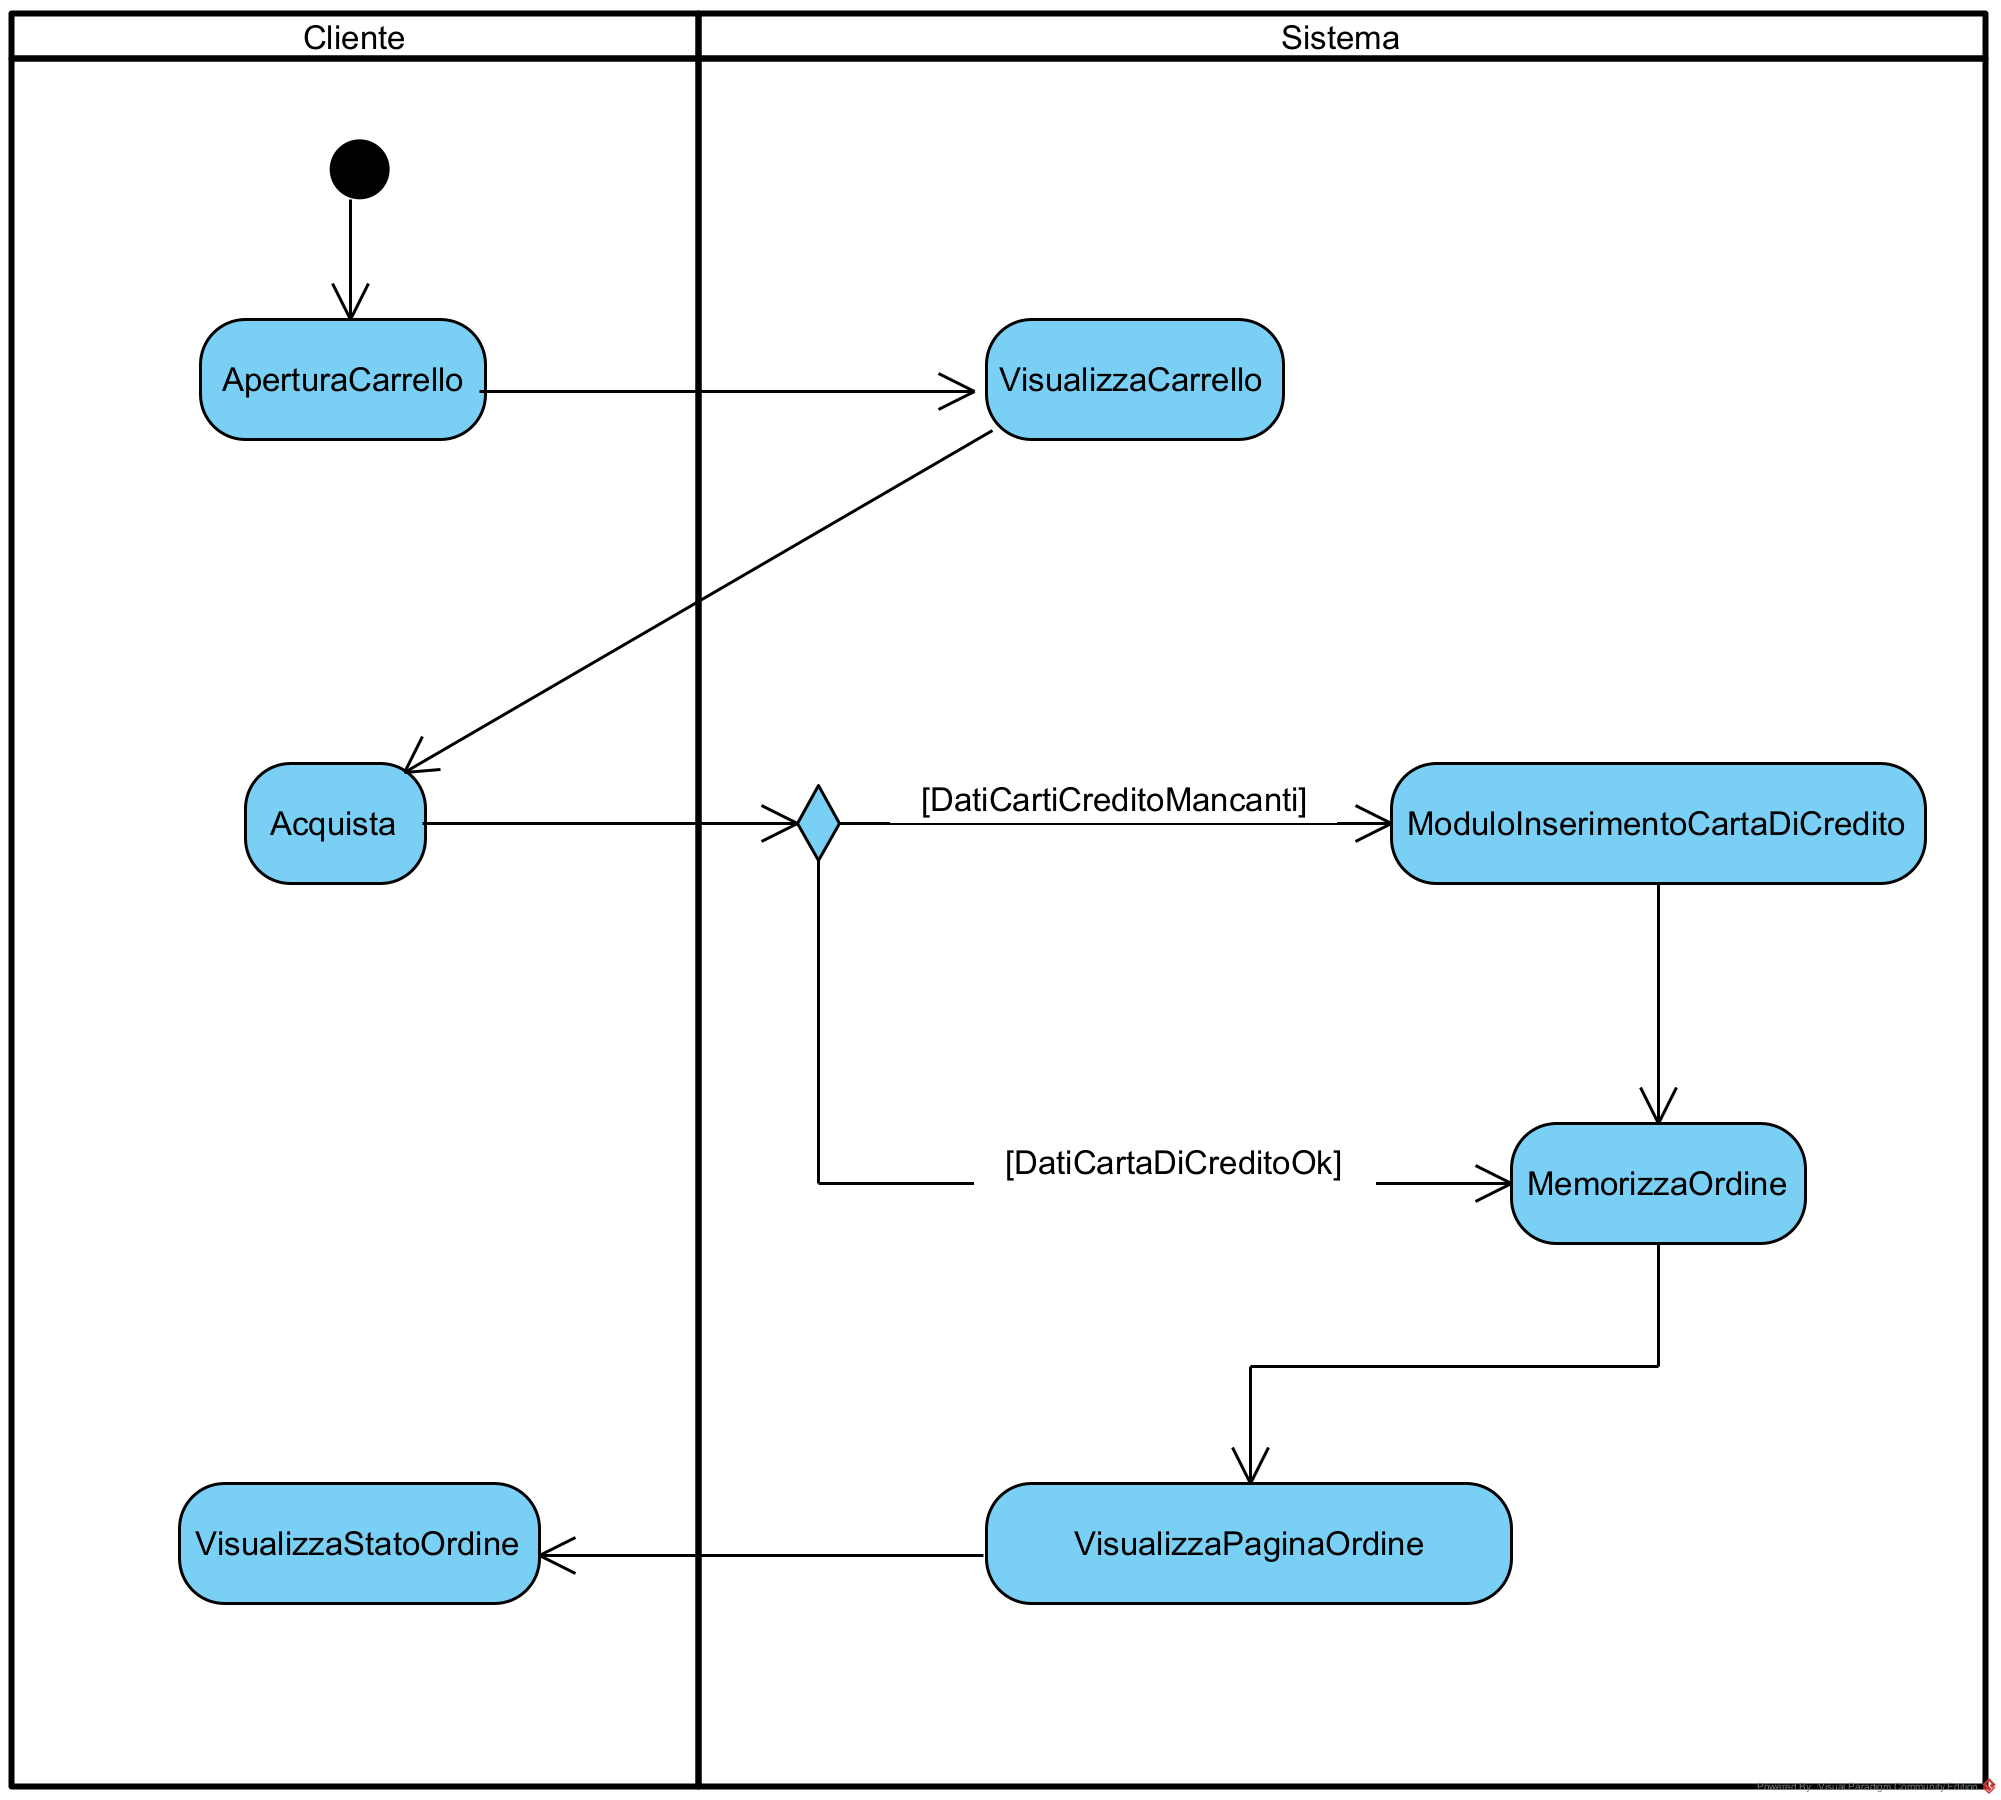
\includegraphics[width=\textwidth]{ActivityDiagram/ClienteAcquistoArticolo}
\end{center}

\subsection{Annullamento}
\begin{center}
\includegraphics[width=\textwidth]{ActivityDiagram/ClienteAnnullamentoOrdine}
\end{center}

\subsection{Vendita}
\begin{center}
\includegraphics[width=\textwidth]{ActivityDiagram/Vendita}
\end{center}

\subsection{Creazione e risposta ad un ticket}
\begin{center}
\includegraphics[width=\textwidth]{ActivityDiagram/Ticket}
\end{center}

\subsection{Aggiunta di un dipendente}
\begin{center}
\includegraphics[width=\textwidth]{ActivityDiagram/AmministratorePersonaleInserisceNuovoDipendente}
\end{center}

\subsection{Modifica di un dipendente}
\begin{center}
\includegraphics[width=\textwidth]{ActivityDiagram/AmministratorePersonaleModificaDipendente}
\end{center}

\subsection{Rimozione di un dipendente}
\begin{center}
\includegraphics[width=\textwidth]{ActivityDiagram/AmministratorePersonaleRimuoveDipendente}
\end{center}

\subsection{Aggiunta di un articolo}
\begin{center}
\includegraphics[width=\textwidth]{ActivityDiagram/AmministratoreCatalogoInserisceNuovoArticolo}
\end{center}

\subsection{Modifica di un articolo}
\begin{center}
\includegraphics[width=\textwidth]{ActivityDiagram/AmministratoreCatalogoModificaArticoloCatalogo}
\end{center}

\subsection{Rimozione di un articolo}
\begin{center}
\includegraphics[width=\textwidth]{ActivityDiagram/AmministratoreCatalogoRimuoveArticolo}
\end{center}

\newpage
\section{Navigational Path}
\subsection{Cliente}
\begin{center}
\includegraphics[width=\textwidth]{NavigationalPath/Cliente}
\end{center}

\subsection{Centralinista}
\begin{center}
\includegraphics[width=\textwidth]{NavigationalPath/Centralinista}
\end{center}

\subsection{Magazziniere}
\begin{center}
\includegraphics[height=300px]{NavigationalPath/Magazziniere}
\end{center}

\subsection{Amministratore Catalogo}
\begin{center}
\includegraphics[height=300px]{NavigationalPath/AmministratoreCatalogo}
\end{center}

\subsection{Amministratore Personale}
\begin{center}
\includegraphics[height=300px]{NavigationalPath/AmministratorePersonale}
\end{center}

\newpage

\newgeometry{top=0.5in,bottom=0.5in,right=0.5in,left=0.2in}

\section{Form Data}
 
 \setlist{leftmargin=5.5mm}
 
 \subsection{Registrazione}
 \setlength\LTleft{0pt}
 \setlength\LTright{0pt}
 \begin{longtable}{|l|l|l|l|l|}
 \hline
 Modulo & Nome & Obbligatorio & Vincoli & Errori\\\hline
 \endhead
 \hline
 \textbf{Registrazione} & Nome & $\checkmark$ & \begin{minipage}{3.5cm}
 \vspace{5pt}
 \begin{itemize}
 \item Lunghezza minima 3 caratteri
 \item Lunghezza massima 24 caratteri
 \item Solo caratteri A-Z, a-z
 \end{itemize}
 \vspace{5pt}
 \end{minipage} & \begin{minipage}{4cm}
 \vspace{5pt}
 \begin{itemize}
 \item Lunghezza inadeguata
 \item Caratteri non consentiti
 \item Campo vuoto
 \end{itemize}
 \vspace{5pt}
 \end{minipage} \\ \hline
 
 \textbf{Registrazione} & Cognome & $\checkmark$ & \begin{minipage}{3.5cm}
 \vspace{5pt}
 \begin{itemize}
 \item Lunghezza minima 3 caratteri
 \item Lunghezza massima 24 caratteri
 \item Solo caratteri A-Z, a-z
 \end{itemize}
 \vspace{5pt}
 \end{minipage} & \begin{minipage}{4cm}
 \vspace{5pt}
 \begin{itemize}
 \item Lunghezza inadeguata
 \item Caratteri non consentiti
 \item Campo vuoto
 \end{itemize}
 \vspace{5pt}
 \end{minipage} \\ \hline
 
 \textbf{Registrazione} & Password & $\checkmark$ & \begin{minipage}{3.5cm}
 \vspace{5pt}
 \begin{itemize}
 \item Lunghezza minima 10 caratteri
 \item Lunghezza massima 64 caratteri
 \end{itemize}
 \vspace{5pt}
 \end{minipage} & \begin{minipage}{4cm}
 \vspace{5pt}
 \begin{itemize}
 \item Lunghezza inadeguata
 \item Campo vuoto
 \end{itemize}
 \vspace{5pt}
 \end{minipage} \\ \hline
 
 \textbf{Registrazione} & Conferma Password & $\checkmark$ & \begin{minipage}{3.5cm}
 \vspace{5pt}
 \begin{itemize}
 \item Lunghezza minima 10 caratteri
 \item Lunghezza massima 64 caratteri
 \item Testo corrispondente al campo ``Password"
 \end{itemize}
 \vspace{5pt}
 \end{minipage} & \begin{minipage}{4cm}
 \vspace{5pt}
 \begin{itemize}
 \item Lunghezza inadeguata
 \item Campo vuoto
 \item Testo non corrispondente al campo ``Password"
 \end{itemize}
 \vspace{5pt}
 \end{minipage} \\ \hline
 
 \textbf{Registrazione} & Email & $\checkmark$ & \begin{minipage}{3.5cm}
 \vspace{5pt}
 \begin{itemize}
 \item Lunghezza minima 10 caratteri
 \item Lunghezza massima 64 caratteri
 \item Testo contenente almeno un punto (U+002E) ed esattamente un carattere ``chiocciola" (U+0040), dei caratteri alfanumerici all'inizio, dei caratteri alfanumerici tra la chiocciola e il punto e una stringa dopo il punto, che deve rientrare nell'elenco dei Top Level Domain attualmente in uso
 \item Testo contenente unicamente i caratteri A-Z, a-z, 0-9 e i caratteri speciali che seguono \begin{verbatim}
 ~!$%^&*_
 =+}{'?-.
 \end{verbatim}
 \end{itemize}
 \vspace{5pt}
 \end{minipage} & \begin{minipage}{4cm}
 \vspace{5pt}
 \begin{itemize}
 \item Lunghezza inadeguata
 \item Campo vuoto
 \item Formato inadeguato ad un indirizzo email
 \end{itemize}
 \vspace{5pt}
 \end{minipage} \\ \hline
 
 \textbf{Registrazione} & Via & $\checkmark$ & \begin{minipage}{3.5cm}
 \vspace{5pt}
 \begin{itemize}
 \item Lunghezza minima 2 caratteri
 \item Lunghezza massima 64 caratteri
 
 \end{itemize}
 \vspace{5pt}
 \end{minipage} & \begin{minipage}{4cm}
 \vspace{5pt}
 \begin{itemize}
 \item Lunghezza inadeguata
 \item Campo vuoto
 \item Formato inadeguato
 \end{itemize}
 \vspace{5pt}
 \end{minipage} \\ \hline
 
 \textbf{Registrazione} & Numero civico & $\checkmark$ & \begin{minipage}{3.5cm}
 \vspace{5pt}
 \begin{itemize}
 \item Lunghezza minima 1 carattere
 \item Lunghezza massima 6 caratteri
 
 \end{itemize}
 \vspace{5pt}
 \end{minipage} & \begin{minipage}{4cm}
 \vspace{5pt}
 \begin{itemize}
 \item Lunghezza inadeguata
 \item Campo vuoto
 \item Formato inadeguato
 \end{itemize}
 \vspace{5pt}
 \end{minipage} \\ \hline
 
\textbf{Registrazione} & Città & $\checkmark$ & \begin{minipage}{3.5cm}
 \vspace{5pt}
 \begin{itemize}
 \item Lunghezza minima 2 caratteri
 \item Lunghezza massima 64 caratteri
 
 \end{itemize}
 \vspace{5pt}
 \end{minipage} & \begin{minipage}{4cm}
 \vspace{5pt}
 \begin{itemize}
 \item Lunghezza inadeguata
 \item Campo vuoto
 \item Formato inadeguato
 \end{itemize}
 \vspace{5pt}
 \end{minipage} \\ \hline
 
\textbf{Registrazione} & Provincia & $\checkmark$ & \begin{minipage}{3.5cm}
 \vspace{5pt}
 \begin{itemize}
 \item Lunghezza di 2 caratteri
 
 \end{itemize}
 \vspace{5pt}
 \end{minipage} & \begin{minipage}{4cm}
 \vspace{5pt}
 \begin{itemize}
 \item Lunghezza inadeguata
 \item Campo vuoto
 \item Formato inadeguato
 \end{itemize}
 \vspace{5pt}
 \end{minipage} \\ \hline
 
\textbf{Registrazione} & CAP & $\checkmark$ & \begin{minipage}{3.5cm}
 \vspace{5pt}
 \begin{itemize}
 \item Lunghezza di 5 caratteri
 
 \end{itemize}
 \vspace{5pt}
 \end{minipage} & \begin{minipage}{4cm}
 \vspace{5pt}
 \begin{itemize}
 \item Lunghezza inadeguata
 \item Campo vuoto
 \item Formato inadeguato
 \end{itemize}
 \vspace{5pt}
 \end{minipage} \\ \hline
 
 \textbf{Registrazione} & Codice Fiscale & $\checkmark$ & \begin{minipage}{3.5cm}
 \vspace{5pt}
 \begin{itemize}
 \item Lunghezza di 16 caratteri
 \item Testo rispettante il formato del codice fiscale, con 6 lettere, due cifre, una lettera, due cifre, cinque caratteri alfanumerici
 \end{itemize}
 \vspace{5pt}
 \end{minipage} & \begin{minipage}{4cm}
 \vspace{5pt}
 \begin{itemize}
 \item Lunghezza inadeguata
 \item Campo vuoto
 \item Formato inadeguato
 \end{itemize}
 \vspace{5pt}
 \end{minipage} \\ \hline
 
 \end{longtable}
 \newpage
 
 \subsection{Autenticazione}
 
 \setlength\LTleft{0pt}
 \setlength\LTright{0pt}
 \begin{longtable}{|l|l|l|l|l|}
 \hline
 Modulo & Nome & Obbligatorio & Vincoli & Errori\\\hline
 \endhead
 \hline
 
 \textbf{Autenticazione} & Email & $\checkmark$ & \begin{minipage}{3.5cm}
 \vspace{5pt}
 \begin{itemize}
 \item Lunghezza minima 10 caratteri
 \item Lunghezza massima 64 caratteri
 \item Testo contenente almeno un punto (U+002E) ed esattamente un carattere ``chiocciola" (U+0040), dei caratteri alfanumerici all'inizio, dei caratteri alfanumerici tra la chiocciola e il punto e una stringa dopo il punto, che deve rientrare nell'elenco dei Top Level Domain attualmente in uso
 \item Testo contenente unicamente i caratteri A-Z, a-z, 0-9 e i caratteri speciali che seguono \begin{verbatim}
 ~!$%^&*_
 =+}{'?-.
 \end{verbatim}
 \end{itemize}
 \vspace{5pt}
 \end{minipage} & \begin{minipage}{4cm}
 \vspace{5pt}
 \begin{itemize}
 \item Lunghezza inadeguata
 \item Campo vuoto
 \item Formato inadeguato ad un indirizzo email
 \end{itemize}
 \vspace{5pt}
 \end{minipage} \\ \hline
 
 \textbf{Autenticazione} & Password & $\checkmark$ & \begin{minipage}{3.5cm}
 \vspace{5pt}
 \begin{itemize}
 \item Lunghezza minima 10 caratteri
 \item Lunghezza massima 64 caratteri
 \end{itemize}
 \vspace{5pt}
 \end{minipage} & \begin{minipage}{4cm}
 \vspace{5pt}
 \begin{itemize}
 \item Lunghezza inadeguata
 \item Campo vuoto
 \end{itemize}
 \vspace{5pt}
 \end{minipage} \\ \hline
 
 \end{longtable}
 
 \subsection{Vendita}
 \setlength\LTleft{0pt}
 \setlength\LTright{0pt}
 \begin{longtable}{|l|l|l|l|l|}
 \hline
 Modulo & Nome & Obbligatorio & Vincoli & Errori\\\hline
 \endhead
 \hline
 \textbf{Vendita} & Nome & $\checkmark$ & \begin{minipage}{3.5cm}
 \vspace{5pt}
 \begin{itemize}
 \item Lunghezza minima 3 caratteri
 \item Lunghezza massima 24 caratteri
 \item Solo caratteri A-Z, a-z, 0-9
 \end{itemize}
 \vspace{5pt}
 \end{minipage} & \begin{minipage}{4cm}
 \vspace{5pt}
 \begin{itemize}
 \item Lunghezza inadeguata
 \item Caratteri non consentiti
 \item Campo vuoto
 \end{itemize}
 \vspace{5pt}
 \end{minipage} \\ \hline
 
 \textbf{Vendita} & Prezzo & $\checkmark$ & \begin{minipage}{3.5cm}
 \vspace{5pt}
 \begin{itemize}
 \item Valore minimo 1€, con incrementi di 0.01€
 \end{itemize}
 \vspace{5pt}
 \end{minipage} & \begin{minipage}{4cm}
 \vspace{5pt}
 \begin{itemize}
 \item Valore minore di 1€
 \item Precisione troppo elevata
 \item Campo vuoto
 \end{itemize}
 \vspace{5pt}
 \end{minipage} \\ \hline
 
 \textbf{Vendita} & Quantità disponibile & $\checkmark$ & \begin{minipage}{3.5cm}
 \vspace{5pt}
 \begin{itemize}
 \item Valore minimo 1
 \end{itemize}
 \vspace{5pt}
 \end{minipage} & \begin{minipage}{4cm}
 \vspace{5pt}
 \begin{itemize}
 \item Valore minore di 1
 \item Valore decimale
 \item Campo vuoto
 \end{itemize}
 \vspace{5pt}
 \end{minipage} \\ \hline
 
 \textbf{Vendita} & Descrizione & $\checkmark$ & \begin{minipage}{3.5cm}
 \vspace{5pt}
 \begin{itemize}
 \item Lunghezza minima 20 caratteri
 \item Lunghezza massima 1024 caratteri
 \end{itemize}
 \vspace{5pt}
 \end{minipage} & \begin{minipage}{4cm}
 \vspace{5pt}
 \begin{itemize}
 \item Lunghezza inadeguata
 \item Campo vuoto
 \end{itemize}
 \vspace{5pt}
 \end{minipage} \\ \hline
 
 \textbf{Vendita} & Rimborsabile & $\checkmark$ & \begin{minipage}{3.5cm}
 \vspace{5pt}
 \begin{itemize}
 \item Valore vero/falso
 \end{itemize}
 \vspace{5pt}
 \end{minipage} & \begin{minipage}{4cm}
 \vspace{5pt}
 \begin{itemize}
 \item Valore inadeguato
 \item Campo vuoto
 \end{itemize}
 \vspace{5pt}
 \end{minipage} \\ \hline
 
 \textbf{Vendita} & Foto & $\checkmark$ & \begin{minipage}{3.5cm}
 \vspace{5pt}
 \begin{itemize}
 \item File di tipo png o jpeg
 \item Almeno 3 file per ogni vendita
 \item Massimo 10 file per vendita
 \end{itemize}
 \vspace{5pt}
 \end{minipage} & \begin{minipage}{4cm}
 \vspace{5pt}
 \begin{itemize}
 \item Numero inadeguato
 \item File di formato errato
 \end{itemize}
 \vspace{5pt}
 \end{minipage} \\ \hline
 
 \end{longtable}
 
 \newpage
 \subsection{Modifica vendita}
 \setlength\LTleft{0pt}
 \setlength\LTright{0pt}
 \begin{longtable}{|l|l|l|l|l|}
 \hline
 Modulo & Nome & Obbligatorio & Vincoli & Errori\\\hline
 \endhead
 \hline
 \textbf{ModificaVendita} & Nome & $\checkmark$ & \begin{minipage}{3.5cm}
 \vspace{5pt}
 \begin{itemize}
 \item Lunghezza minima 3 caratteri
 \item Lunghezza massima 24 caratteri
 \item Solo caratteri A-Z, a-z, 0-9
 \end{itemize}
 \vspace{5pt}
 \end{minipage} & \begin{minipage}{4cm}
 \vspace{5pt}
 \begin{itemize}
 \item Lunghezza inadeguata
 \item Caratteri non consentiti
 \item Campo vuoto
 \end{itemize}
 \vspace{5pt}
 \end{minipage} \\ \hline
 
 \textbf{ModificaVendita} & Prezzo & $\checkmark$ & \begin{minipage}{3.5cm}
 \vspace{5pt}
 \begin{itemize}
 \item Valore minimo 1€, con incrementi di 0.01€
 \end{itemize}
 \vspace{5pt}
 \end{minipage} & \begin{minipage}{4cm}
 \vspace{5pt}
 \begin{itemize}
 \item Valore minore di 1€
 \item Precisione troppo elevata
 \item Campo vuoto
 \end{itemize}
 \vspace{5pt}
 \end{minipage} \\ \hline
 
 \textbf{ModificaVendita} & Quantità disponibile & $\checkmark$ & \begin{minipage}{3.5cm}
 \vspace{5pt}
 \begin{itemize}
 \item Valore minimo 1
 \end{itemize}
 \vspace{5pt}
 \end{minipage} & \begin{minipage}{4cm}
 \vspace{5pt}
 \begin{itemize}
 \item Valore minore di 1
 \item Valore decimale
 \item Campo vuoto
 \end{itemize}
 \vspace{5pt}
 \end{minipage} \\ \hline
 
 \textbf{ModificaVendita} & Descrizione & $\checkmark$ & \begin{minipage}{3.5cm}
 \vspace{5pt}
 \begin{itemize}
 \item Lunghezza minima 20 caratteri
 \item Lunghezza massima 1024 caratteri
 \end{itemize}
 \vspace{5pt}
 \end{minipage} & \begin{minipage}{4cm}
 \vspace{5pt}
 \begin{itemize}
 \item Lunghezza inadeguata
 \item Campo vuoto
 \end{itemize}
 \vspace{5pt}
 \end{minipage} \\ \hline
 
 \textbf{ModificaVendita} & Rimborsabile & $\checkmark$ & \begin{minipage}{3.5cm}
 \vspace{5pt}
 \begin{itemize}
 \item Valore vero/falso
 \end{itemize}
 \vspace{5pt}
 \end{minipage} & \begin{minipage}{4cm}
 \vspace{5pt}
 \begin{itemize}
 \item Valore inadeguato
 \item Campo vuoto
 \end{itemize}
 \vspace{5pt}
 \end{minipage} \\ \hline
 
 \textbf{ModificaVendita} & Foto & $\checkmark$ & \begin{minipage}{3.5cm}
 \vspace{5pt}
 \begin{itemize}
 \item File di tipo png o jpeg
 \item Almeno 3 file per ogni vendita
 \item Massimo 10 file per vendita
 \end{itemize}
 \vspace{5pt}
 \end{minipage} & \begin{minipage}{4cm}
 \vspace{5pt}
 \begin{itemize}
 \item Numero inadeguato
 \item File di formato errato
 \end{itemize}
 \vspace{5pt}
 \end{minipage} \\ \hline
 
 \end{longtable}
 
 \newpage
 \subsection{Inserimento dipendente}
 
 \setlength\LTleft{0pt}
 \setlength\LTright{0pt}
 \begin{longtable}{|l|l|l|l|l|}
 \hline
 Modulo & Nome & Obbligatorio & Vincoli & Errori\\\hline
 \endhead
 \hline
 \textbf{InserimentoDipendente} & Nome & $\checkmark$ & \begin{minipage}{3.5cm}
 \vspace{5pt}
 \begin{itemize}
 \item Lunghezza minima 3 caratteri
 \item Lunghezza massima 24 caratteri
 \item Solo caratteri A-Z, a-z
 \end{itemize}
 \vspace{5pt}
 \end{minipage} & \begin{minipage}{4cm}
 \vspace{5pt}
 \begin{itemize}
 \item Lunghezza inadeguata
 \item Caratteri non consentiti
 \item Campo vuoto
 \end{itemize}
 \vspace{5pt}
 \end{minipage} \\ \hline
 
 \textbf{InserimentoDipendente} & Cognome & $\checkmark$ & \begin{minipage}{3.5cm}
 \vspace{5pt}
 \begin{itemize}
 \item Lunghezza minima 3 caratteri
 \item Lunghezza massima 24 caratteri
 \item Solo caratteri A-Z, a-z
 \end{itemize}
 \vspace{5pt}
 \end{minipage} & \begin{minipage}{4cm}
 \vspace{5pt}
 \begin{itemize}
 \item Lunghezza inadeguata
 \item Caratteri non consentiti
 \item Campo vuoto
 \end{itemize}
 \vspace{5pt}
 \end{minipage} \\ \hline
 
 \textbf{InserimentoDipendente} & Email & $\checkmark$ & \begin{minipage}{3.5cm}
 \vspace{5pt}
 \begin{itemize}
 \item Lunghezza minima 10 caratteri
 \item Lunghezza massima 64 caratteri
 \item Testo contenente almeno un punto (U+002E) ed esattamente un carattere ``chiocciola" (U+0040), dei caratteri alfanumerici all'inizio, dei caratteri alfanumerici tra la chiocciola e il punto e una stringa dopo il punto, che deve rientrare nell'elenco dei Top Level Domain attualmente in uso
 \item Testo contenente unicamente i caratteri A-Z, a-z, 0-9 e i caratteri speciali che seguono \begin{verbatim}
 ~!$%^&*_
 =+}{'?-.
 \end{verbatim}
 \end{itemize}
 \vspace{5pt}
 \end{minipage} & \begin{minipage}{4cm}
 \vspace{5pt}
 \begin{itemize}
 \item Lunghezza inadeguata
 \item Campo vuoto
 \item Formato inadeguato ad un indirizzo email
 \end{itemize}
 \vspace{5pt}
 \end{minipage} \\ \hline
 
\textbf{Registrazione} & Via & $\checkmark$ & \begin{minipage}{3.5cm}
 \vspace{5pt}
 \begin{itemize}
 \item Lunghezza minima 2 caratteri
 \item Lunghezza massima 64 caratteri
 
 \end{itemize}
 \vspace{5pt}
 \end{minipage} & \begin{minipage}{4cm}
 \vspace{5pt}
 \begin{itemize}
 \item Lunghezza inadeguata
 \item Campo vuoto
 \item Formato inadeguato
 \end{itemize}
 \vspace{5pt}
 \end{minipage} \\ \hline
 
 \textbf{Registrazione} & Numero civico & $\checkmark$ & \begin{minipage}{3.5cm}
 \vspace{5pt}
 \begin{itemize}
 \item Lunghezza minima 1 carattere
 \item Lunghezza massima 6 caratteri
 
 \end{itemize}
 \vspace{5pt}
 \end{minipage} & \begin{minipage}{4cm}
 \vspace{5pt}
 \begin{itemize}
 \item Lunghezza inadeguata
 \item Campo vuoto
 \item Formato inadeguato
 \end{itemize}
 \vspace{5pt}
 \end{minipage} \\ \hline
 
\textbf{Registrazione} & Città & $\checkmark$ & \begin{minipage}{3.5cm}
 \vspace{5pt}
 \begin{itemize}
 \item Lunghezza minima 2 caratteri
 \item Lunghezza massima 64 caratteri
 
 \end{itemize}
 \vspace{5pt}
 \end{minipage} & \begin{minipage}{4cm}
 \vspace{5pt}
 \begin{itemize}
 \item Lunghezza inadeguata
 \item Campo vuoto
 \item Formato inadeguato
 \end{itemize}
 \vspace{5pt}
 \end{minipage} \\ \hline
 
\textbf{Registrazione} & Provincia & $\checkmark$ & \begin{minipage}{3.5cm}
 \vspace{5pt}
 \begin{itemize}
 \item Lunghezza di 2 caratteri
 
 \end{itemize}
 \vspace{5pt}
 \end{minipage} & \begin{minipage}{4cm}
 \vspace{5pt}
 \begin{itemize}
 \item Lunghezza inadeguata
 \item Campo vuoto
 \item Formato inadeguato
 \end{itemize}
 \vspace{5pt}
 \end{minipage} \\ \hline
 
\textbf{Registrazione} & CAP & $\checkmark$ & \begin{minipage}{3.5cm}
 \vspace{5pt}
 \begin{itemize}
 \item Lunghezza di 5 caratteri
 
 \end{itemize}
 \vspace{5pt}
 \end{minipage} & \begin{minipage}{4cm}
 \vspace{5pt}
 \begin{itemize}
 \item Lunghezza inadeguata
 \item Campo vuoto
 \item Formato inadeguato
 \end{itemize}
 \vspace{5pt}
 \end{minipage} \\ \hline
 
 \textbf{InserimentoDipendente} & Codice Fiscale & $\checkmark$ & \begin{minipage}{3.5cm}
 \vspace{5pt}
 \begin{itemize}
 \item Lunghezza di 16 caratteri
 \item Testo rispettante il formato del codice fiscale, con 6 lettere, due cifre, una lettera, due cifre, cinque caratteri alfanumerici
 \end{itemize}
 \vspace{5pt}
 \end{minipage} & \begin{minipage}{4cm}
 \vspace{5pt}
 \begin{itemize}
 \item Lunghezza inadeguata
 \item Campo vuoto
 \item Formato inadeguato
 \end{itemize}
 \vspace{5pt}
 \end{minipage} \\ \hline
 
 \textbf{InserimentoDipendente} & Ruolo & $\checkmark$ & \begin{minipage}{3.8cm}
 \vspace{5pt}
 \begin{itemize}
 \item Uno dei seguenti valori: \begin{verbatim}
 [ 
 'magazziniere',
 'centralinista',
 'amministratore
 personale',
 'amministratore
 catalogo' 
 ]
 \end{verbatim}
 \end{itemize}
 \vspace{5pt}
 \end{minipage} & \begin{minipage}{4cm}
 \vspace{5pt}
 \begin{itemize}
 \item Valore invalido
 \item Campo vuoto
 \end{itemize}
 \vspace{5pt}
 \end{minipage} \\ \hline
 \end{longtable}
 
 
 \newpage
 \subsection{Modifica dipendente}
 
 \setlength\LTleft{0pt}
 \setlength\LTright{0pt}
 \begin{longtable}{|l|l|l|l|l|}
 \hline
 Modulo & Nome & Obbligatorio & Vincoli & Errori\\\hline
 \endhead
 \hline
 \textbf{ModificaDipendente} & Nome & $\checkmark$ & \begin{minipage}{3.5cm}
 \vspace{5pt}
 \begin{itemize}
 \item Lunghezza minima 3 caratteri
 \item Lunghezza massima 24 caratteri
 \item Solo caratteri A-Z, a-z
 \end{itemize}
 \vspace{5pt}
 \end{minipage} & \begin{minipage}{4cm}
 \vspace{5pt}
 \begin{itemize}
 \item Lunghezza inadeguata
 \item Caratteri non consentiti
 \item Campo vuoto
 \end{itemize}
 \vspace{5pt}
 \end{minipage} \\ \hline
 
 \textbf{ModificaDipendente} & Cognome & $\checkmark$ & \begin{minipage}{3.5cm}
 \vspace{5pt}
 \begin{itemize}
 \item Lunghezza minima 3 caratteri
 \item Lunghezza massima 24 caratteri
 \item Solo caratteri A-Z, a-z
 \end{itemize}
 \vspace{5pt}
 \end{minipage} & \begin{minipage}{4cm}
 \vspace{5pt}
 \begin{itemize}
 \item Lunghezza inadeguata
 \item Caratteri non consentiti
 \item Campo vuoto
 \end{itemize}
 \vspace{5pt}
 \end{minipage} \\ \hline
 
 \textbf{ModificaDipendente} & Email & $\checkmark$ & \begin{minipage}{3.5cm}
 \vspace{5pt}
 \begin{itemize}
 \item Lunghezza minima 10 caratteri
 \item Lunghezza massima 64 caratteri
 \item Testo contenente almeno un punto (U+002E) ed esattamente un carattere ``chiocciola" (U+0040), dei caratteri alfanumerici all'inizio, dei caratteri alfanumerici tra la chiocciola e il punto e una stringa dopo il punto, che deve rientrare nell'elenco dei Top Level Domain attualmente in uso
 \item Testo contenente unicamente i caratteri A-Z, a-z, 0-9 e i caratteri speciali che seguono \begin{verbatim}
 ~!$%^&*_
 =+}{'?-.
 \end{verbatim}
 \end{itemize}
 \vspace{5pt}
 \end{minipage} & \begin{minipage}{4cm}
 \vspace{5pt}
 \begin{itemize}
 \item Lunghezza inadeguata
 \item Campo vuoto
 \item Formato inadeguato ad un indirizzo email
 \end{itemize}
 \vspace{5pt}
 \end{minipage} \\ \hline
 
 \textbf{ModificaDipendente} & Indirizzo & $\checkmark$ & \begin{minipage}{3.5cm}
 \vspace{5pt}
 \begin{itemize}
 \item Lunghezza minima 5 caratteri
 \item Lunghezza massima 64 caratteri
 \item Testo rispettante il formato previsto dal documento allegato
 \begin{verbatim}
 standard_
 composizione_
 indirizzi.pdf
 \end{verbatim} 
 
 \end{itemize}
 \vspace{5pt}
 \end{minipage} & \begin{minipage}{4cm}
 \vspace{5pt}
 \begin{itemize}
 \item Lunghezza inadeguata
 \item Campo vuoto
 \item Formato inadeguato
 \end{itemize}
 \vspace{5pt}
 \end{minipage} \\ \hline
 
 \textbf{ModificaDipendente} & Codice Fiscale & $\checkmark$ & \begin{minipage}{3.5cm}
 \vspace{5pt}
 \begin{itemize}
 \item Lunghezza di 16 caratteri
 \item Testo rispettante il formato del codice fiscale, con 6 lettere, due cifre, una lettera, due cifre, cinque caratteri alfanumerici
 \end{itemize}
 \vspace{5pt}
 \end{minipage} & \begin{minipage}{4cm}
 \vspace{5pt}
 \begin{itemize}
 \item Lunghezza inadeguata
 \item Campo vuoto
 \item Formato inadeguato
 \end{itemize}
 \vspace{5pt}
 \end{minipage} \\ \hline
 
 \textbf{ModificaDipendente} & Ruolo & $\checkmark$ & \begin{minipage}{3.8cm}
 \vspace{5pt}
 \begin{itemize}
 \item Uno dei seguenti valori: \begin{verbatim}
 [ 
 'magazziniere',
 'centralinista',
 'amministratore
 personale',
 'amministratore
 catalogo' 
 ]
 \end{verbatim}
 \end{itemize}
 \vspace{5pt}
 \end{minipage} & \begin{minipage}{4cm}
 \vspace{5pt}
 \begin{itemize}
 \item Valore invalido
 \item Campo vuoto
 \end{itemize}
 \vspace{5pt}
 \end{minipage} \\ \hline
 \end{longtable}
 
 \newpage
 \subsection{Creazione ticket}
 
 \setlength\LTleft{0pt}
 \setlength\LTright{0pt}
 \begin{longtable}{|l|l|l|l|l|}
 \hline
 Modulo & Nome & Obbligatorio & Vincoli & Errori\\\hline
 \endhead
 \hline
 \textbf{CreazioneTicket} & Tipologia & $\checkmark$ & \begin{minipage}{4cm}
 \vspace{5pt}
 \begin{itemize}
 \item Uno dei seguenti valori: \begin{verbatim}
 [ 
 'spedizione',
 'pagamento',
 'amministrativo',
 'vendita',
 'altro' 
 ]
 \end{verbatim}
 \end{itemize}
 \vspace{5pt}
 \end{minipage} & \begin{minipage}{4cm}
 \vspace{5pt}
 \begin{itemize}
 \item Lunghezza inadeguata
 \item Campo vuoto
 \item Formato inadeguato
 \end{itemize}
 \vspace{5pt}
 \end{minipage} \\ \hline
 
 \textbf{CreazioneTicket} & Messaggio & $\checkmark$ & \begin{minipage}{3.5cm}
 \vspace{5pt}
 \begin{itemize}
 \item Lunghezza minima di 16 caratteri
 \item Lunghezza massima di 1024 caratteri
 \end{itemize}
 \vspace{5pt}
 \end{minipage} & \begin{minipage}{4cm}
 \vspace{5pt}
 \begin{itemize}
 \item Lunghezza inadeguata
 \item Campo vuoto
 \end{itemize}
 \vspace{5pt}
 \end{minipage} \\ \hline
 \end{longtable}
 
 \newpage
 \subsection{Risposta ticket}
 
 \setlength\LTleft{0pt}
 \setlength\LTright{0pt}
 \begin{longtable}{|l|l|l|l|l|}
 \hline
 Modulo & Nome & Obbligatorio & Vincoli & Errori\\\hline
 \endhead
 \hline
 \textbf{RispostaTicket} & Messaggio & $\checkmark$ & \begin{minipage}{3.5cm}
 \vspace{5pt}
 \begin{itemize}
 \item Lunghezza minima di 16 caratteri
 \item Lunghezza massima di 1024 caratteri
 \end{itemize}
 \vspace{5pt}
 \end{minipage} & \begin{minipage}{4cm}
 \vspace{5pt}
 \begin{itemize}
 \item Lunghezza inadeguata
 \item Campo vuoto
 \end{itemize}
 \vspace{5pt}
 \end{minipage} \\ \hline
 \end{longtable}
 
 \newpage
 
 \subsection{Conferma ordine}
 
 \setlength\LTleft{0pt}
 \setlength\LTright{0pt}
 \begin{longtable}{|l|l|l|l|l|}
 \hline
 Modulo & Nome & Obbligatorio & Vincoli & Errori\\\hline
 \endhead
 \hline
 \textbf{ConfermaOrdine} & CodiceTracciamento & $\checkmark$ & \begin{minipage}{3.5cm}
 \vspace{5pt}
 \begin{itemize}
 \item Lunghezza minima di 8 caratteri
 \item Lunghezza massima di 128 caratteri
 \end{itemize}
 \vspace{5pt}
 \end{minipage} & \begin{minipage}{4cm}
 \vspace{5pt}
 \begin{itemize}
 \item Lunghezza inadeguata
 \item Campo vuoto
 \end{itemize}
 \vspace{5pt}
 \end{minipage} \\ \hline
 \end{longtable}

\newpage

\section{Mock up}
\subsection{Generali}
\subsubsection{Pagina iniziale}
\label{mockup:paginainiziale}
Un qualsiasi utente che si connette al sito, visualizzerà una pagina iniziale dalla quale è possibile ricercare articoli, autenticarsi o registrarsi:

\begin{center}
\includegraphics[height=0.3\textheight]{Mockup/PaginaIniziale}
\end{center}

\subsubsection{Autenticazione}
\label{mockup:auth}
Un utente che desidera autenticarsi può utilizzare il tasto ``Autenticati" dalla pagina iniziale (\ref{mockup:paginainiziale}).
Viene quindi mostrato un modulo per l'inserimento di email e password:

\begin{center}
\includegraphics[height=0.3\textheight]{Mockup/Autenticazione}
\end{center}


\newpage

\subsubsection{Conferma delle operazioni}
Dopo ogni operazione di inserimento o modifica, viene visualizzata una pagina generica che mostra l'esito dell'operazione:

\begin{center}
\includegraphics[height=0.3\textheight]{Mockup/Conferma}
\end{center}

\newpage

\subsection{Cliente}
\subsubsection{Registrazione}
Un cliente che non ha ancora un account, può registrarsi dalla pagina iniziale. Viene mostrato un modulo per l'inserimento dei dati necessari:
\begin{center}
\includegraphics[height=0.3\textheight]{Mockup/Cliente/Registrazione}
\end{center}

Se uno o più campi contengono degli errori, viene mostrato un avviso:
\begin{center}
\includegraphics[height=0.3\textheight]{Mockup/Cliente/ErroreRegistrazione}
\end{center}

\newpage

\subsubsection{Pagina iniziale}
\label{mockup:clienteauth}
Un cliente che si autentica viene rimandato ad una versione della pagina iniziale in cui viene riconosciuto che il cliente è attualmente autenticato, con tasti per raggiungere l'area venditori (\ref{mockup:areavenditori}) e l'assistenza clienti (\ref{mockup:assistenzaclienti}):

\begin{center}
\includegraphics[height=0.3\textheight]{Mockup/Cliente/PaginaInizialeAutenticato}
\end{center}

\subsubsection{Ricerca di un articolo}
\label{mockup:clientericerca}
Un cliente interessato ad acquistare un articolo può ricercare il suo nome tramite la barra di ricerca in alto nella pagina. Viene quindi rimandato ad un elenco di risultati:

\begin{center}
\includegraphics[height=0.3\textheight]{Mockup/Cliente/Ricerca}
\end{center}

\newpage

\subsubsection{Dettagli di un articolo}
\label{mockup:clientedettagli}
Dai risultati della ricerca, un cliente può selezionare un articolo per visualizzarne i dettagli:

\begin{center}
\includegraphics[height=0.3\textheight]{Mockup/Cliente/DettagliArticolo}
\end{center}

\subsubsection{Aggiunta al carrello}
\label{mockup:clientecarrello}
Dai dettagli di un articolo, un cliente può decidere di aggiungere l'articolo al carrello:

\begin{center}
\includegraphics[height=0.3\textheight]{Mockup/Cliente/Carrello}
\end{center}

\newpage

Se un utente non autenticato prova ad aggiungere un articolo, viene mostrato un messaggio di errore e viene chiesto di autenticarsi o registrarsi:
\begin{center}
\includegraphics[height=0.3\textheight]{Mockup/Cliente/CarrelloRichiestaLogin}
\end{center}

\subsubsection{Acquisto}
Dopo aver aggiunto almeno un articolo al carrello, un cliente può decidere di acquistare. Viene mostrata una pagina con un riepilogo dei dettagli dell'ordine:

\begin{center}
\includegraphics[height=0.3\textheight]{Mockup/Cliente/ConfermaAcquisto}
\end{center}

\newpage
Se l'utente non ha ancora registrato una carta di credito, gli viene mostrato un modulo per l'inserimento dei dati necessari:
\begin{center}
\includegraphics[height=0.3\textheight]{Mockup/Cliente/DettagliCarta}
\end{center}

\subsubsection{Servizio Clienti}
\label{mockup:assistenzaclienti}
Se un cliente ha necessità di comunicare con il servizio clienti, può usare il tasto dedicato dalla pagina iniziale (\ref{mockup:clienteauth}). Viene mostrato un elenco di ticket aperti:

\begin{center}
\includegraphics[height=0.3\textheight]{Mockup/Cliente/ElencoTicket}
\end{center}

\newpage

\subsubsection{Dettagli Ticket}
Dall'elenco dei ticket, un cliente può selezionarne uno per visualizzare tutti i messaggi:

\begin{center}
\includegraphics[height=0.3\textheight]{Mockup/Cliente/DettagliTicket}
\end{center}

\subsubsection{Risposta Ticket}
Dai dettagli di un ticket, un cliente può inserire un nuovo messaggio:

\begin{center}
\includegraphics[height=0.3\textheight]{Mockup/Cliente/RispostaTicket}
\end{center}

\newpage

\subsubsection{Creazione Ticket}
Dall'elenco dei ticket, un cliente può creare un nuovo ticket:

\begin{center}
\includegraphics[height=0.3\textheight]{Mockup/Cliente/NuovoTicket}
\end{center}

\subsubsection{Area Venditori}
\label{mockup:areavenditori}
Se un cliente vuole vendere un articolo, può usare il tasto dedicato dalla pagina iniziale (\ref{mockup:clienteauth}). Viene mostrata la pagina principale del'area venditori:

\begin{center}
\includegraphics[height=0.3\textheight]{Mockup/Cliente/AreaVenditori}
\end{center}

\newpage

\subsubsection{Ricerca Vendita}
Dall'area venditori, un cliente può ricercare tra gli articoli che ha in vendita:

\begin{center}
\includegraphics[height=0.3\textheight]{Mockup/Cliente/ElencoVendite}
\end{center}

\subsubsection{Dettagli Vendita}
Dai risultati di una ricerca, un cliente può selezionarne uno per visualizzarne i dettagli:

\begin{center}
\includegraphics[height=0.3\textheight]{Mockup/Cliente/DettagliVendita}
\end{center}

\newpage

\subsubsection{Modifica Vendita}
Dalla pagina dei dettagli di una vendita, un cliente può modificarne i dettagli:

\begin{center}
\includegraphics[height=0.3\textheight]{Mockup/Cliente/NuovaVendita}
\end{center}

\subsubsection{Creazione Vendita}
Dall'area venditori, un cliente può creare una nuova vendita:

\begin{center}
\includegraphics[height=0.3\textheight]{Mockup/Cliente/NuovaVendita}
\end{center}

\newpage

\subsection{Centralinista}
\subsubsection{Pagina iniziale}
Dopo essersi autenticato, un centralinista viene reindirizzato alla sua pagina principale, in cui può decidere se visualizzare i ticket o gli ordini da confermare:
\begin{center}
\includegraphics[height=0.3\textheight]{Mockup/Centralinista/PaginaIniziale}
\end{center}

\subsubsection{Gestione Ticket}
Dopo aver selezionato ``Ticket" dalla pagina iniziale, il centralinista visualizza l'elenco dei ticket in attesa di risposta:

\begin{center}
\includegraphics[height=0.3\textheight]{Mockup/Centralinista/ElencoTicket}
\end{center}

\newpage

\subsubsection{Dettagli Ticket}
Dall'elenco dei ticket, un centralinista può selezionarne uno per visualizzare tutti i messaggi:

\begin{center}
\includegraphics[height=0.3\textheight]{Mockup/Centralinista/DettagliTicket}
\end{center}

\subsubsection{Risposta Ticket}
Dai dettagli di un ticket, un centralinista può inserire un nuovo messaggio:

\begin{center}
\includegraphics[height=0.3\textheight]{Mockup/Centralinista/RispostaTicket}
\end{center}

\newpage

\subsubsection{Gestione Vendite}
Dopo aver selezionato ``Vendite" dalla pagina iniziale, il centralinista visualizza l'elenco delle vendite in attesa di conferma:

\begin{center}
\includegraphics[height=0.3\textheight]{Mockup/Centralinista/ElencoVendite}
\end{center}

\subsubsection{Dettagli Vendita}
Dall'elenco delle vendite, un centralinista può selezionarne una per visualizzare tutti i dettagli e decidere se accettare o rifiutare l'inserimento:

\begin{center}
\includegraphics[height=0.3\textheight]{Mockup/Centralinista/DettagliVendita}
\end{center}

\newpage

\subsection{Magazziniere}
\subsubsection{Pagina iniziale}
Dopo essersi autenticato, un magazziniere viene rimandato alla sua pagina iniziale, dalla quale può scegliere se visualizzare gli ordini in attesa di spedizione o i rimborsi in attesa di conferma:

\begin{center}
\includegraphics[height=0.3\textheight]{Mockup/Magazziniere/PaginaIniziale}
\end{center}

\subsubsection{Elenco ordini}
Dopo aver scelto ``Spedizione ordini" dalla pagina iniziale, viene mostrato un elenco di ordini in attesa di spedizione:

\begin{center}
\includegraphics[height=0.3\textheight]{Mockup/Magazziniere/Elenco}
\end{center}

\newpage

\subsubsection{Dettagli ordine}
Dall'elenco degli ordini, un magazziniere può selezionarne uno per visualizzarne i dettagli, come identificativo del prodotto, nome del destinatario e indirizzo di destinazione, con un campo per inserire il codice del tracciamento della spedizione:

\begin{center}
\includegraphics[height=0.3\textheight]{Mockup/Magazziniere/DettagliOrdine}
\end{center}

\subsubsection{Elenco rimborsi}
Dopo aver scelto ``Gestione rimborsi" dalla pagina iniziale, viene mostrato un elenco di ordini in attesa di conferma:

\begin{center}
\includegraphics[height=0.3\textheight]{Mockup/Magazziniere/Elenco}
\end{center}

\newpage

\subsubsection{Dettagli rimborso}
Dall'elenco dei rimborsi, un magazziniere può selezionarne uno per visualizzarne i dettagli e confermare di averlo ricevuto:

\begin{center}
\includegraphics[height=0.3\textheight]{Mockup/Magazziniere/DettagliRimborso}
\end{center}

\newpage

\subsection{Amministratore Catalogo}
\subsubsection{Pagina Iniziale}
Dopo essersi autenticato, un amministratore del catalogo viene rimandato alla pagina per la gestione delle vendite, da cui può cercare tra le vendite esistenti o inserirne una nuova:

\begin{center}
\includegraphics[height=0.3\textheight]{Mockup/AmministratoreCatalogo/PaginaIniziale}
\end{center}

\subsubsection{Nuovo Articolo}
Dalla sua pagina iniziale, un amministratore del catalogo può aggiungere un nuovo articolo con il tasto dedicato. Viene quindi rimandato ad un modulo per l'inserimento dei dati necessari:

\begin{center}
\includegraphics[height=0.3\textheight]{Mockup/AmministratoreCatalogo/NuovoArticolo}
\end{center}

\newpage

\subsubsection{Ricerca}
Dalla sua pagina iniziale, un amministratore del catalogo può ricercare tra gli articoli in vendita sulla piattaforma:

\begin{center}
\includegraphics[height=0.3\textheight]{Mockup/AmministratoreCatalogo/Ricerca}
\end{center}

\subsubsection{Dettagli Articolo}
Dai risultati di una ricerca, un amministratore del catalogo può selezionarne una per visualizzarne i dettagli:

\begin{center}
\includegraphics[height=0.3\textheight]{Mockup/AmministratoreCatalogo/DettagliProdotto}
\end{center}

\newpage

\subsubsection{Modifica Articolo}
Dalla pagina dei dettagli di un articolo, un amministratore del catalogo può modificarne i dettagli:

\begin{center}
\includegraphics[height=0.3\textheight]{Mockup/AmministratoreCatalogo/NuovoArticolo}
\end{center}

\subsubsection{Creazione Vendita}
Dalla sua pagina principale, un amministratore del catalogo può creare un nuovo articolo:

\begin{center}
\includegraphics[height=0.3\textheight]{Mockup/AmministratoreCatalogo/NuovoArticolo}
\end{center}

\newpage

\subsection{Amministratore Personale}
\subsubsection{Pagina Iniziale}
Dopo essersi autenticato, un amministratore del personale viene rimandato alla pagina per la gestione del personale, da cui può cercare tra i dipendenti esistenti o inserirne:

\begin{center}
\includegraphics[height=0.3\textheight]{Mockup/AmministratorePersonale/PaginaIniziale}
\end{center}

\subsubsection{Registrazione dipendente}
\label{mockup:registrazionedipendente}
Dalla sua pagina principale, un amministratore del personale può registrare un nuovo dipendente:

\begin{center}
\includegraphics[height=0.3\textheight]{Mockup/AmministratorePersonale/Registrazione}
\end{center}

\newpage

A registrazione avvenuta, viene mostrata una pagina contenente la password generata dal sistema:

\begin{center}
\includegraphics[height=0.3\textheight]{Mockup/AmministratorePersonale/EsitoRegistrazione}
\end{center}


\subsubsection{Ricerca}
Dalla sua pagina iniziale, un amministratore del personale può ricercare tra i dipendenti della piattaforma:

\begin{center}
\includegraphics[height=0.3\textheight]{Mockup/AmministratorePersonale/Ricerca}
\end{center}

\newpage

\subsubsection{Dettagli Dipendente}
Dai risultati di una ricerca, un amministratore del personale può selezionarne uno per visualizzarne i dettagli:

\begin{center}
\includegraphics[height=0.3\textheight]{Mockup/AmministratorePersonale/Dettagli}
\end{center}

Con il tasto ``Modifica password" viene generata una nuova password e viene visualizzata la stessa pagina di conferma della registrazione (\ref{mockup:registrazionedipendente}).


\subsubsection{Modifica Dipendente}
Dalla pagina dei dettagli di un dipendente, un amministratore del personale può modificarne i dettagli:

\begin{center}
\includegraphics[height=0.3\textheight]{Mockup/AmministratorePersonale/Registrazione}
\end{center}

\newpage

\newpage

%\newgeometry{a4paper,textwidth=345pt,textheight=598pt}

\end{document}
